\documentclass[review]{elsarticle}

\usepackage{multirow}
\usepackage{lineno}
\usepackage{xspace}
\usepackage{threeparttable}
\modulolinenumbers[5]

%% Journal name here
\journal{Annals of Nuclear Energy}

%% `Elsevier LaTeX' style
\bibliographystyle{elsarticle-num}
%%%%%%%%%%%%%%%%%%%%%%%

%%%% packages and definitions (optional)
\usepackage{placeins}
\usepackage{booktabs} % nice rules (thick lines) for tables
\usepackage{microtype} % improves typography for PDF
\usepackage{hhline}

\usepackage{booktabs}
\usepackage{threeparttable, tablefootnote}

\usepackage{tabularx}

\usepackage{mathtools}
\usepackage{amsmath}
\usepackage{amssymb}
\usepackage{stmaryrd}
\usepackage{bm}
\usepackage{subcaption}
\usepackage{siunitx}

%% Special typesetting for Cyclus
\newcommand{\Cyclus}{\textsc{Cyclus}\xspace}%
\newcommand{\Cycamore}{\textsc{Cycamore}\xspace}%
\graphicspath{{images/}}

% tikz %
\usepackage{tikz}
\usepackage{tkz-euclide}
\usetikzlibrary{positioning, arrows, decorations, shapes, fit, backgrounds}
\usetikzlibrary{shapes.geometric,arrows}
\definecolor{illiniblue}{HTML}{B1C6E2}
\definecolor{illiniorange}{HTML}{f8c2a2}
\definecolor{green}{HTML}{c2e2b1}
\tikzstyle{process} = [rectangle, rounded corners, thick, minimum width=7cm, minimum height=1cm, text centered, draw=black, fill=illiniblue, text width=18em]
\tikzstyle{object} = [ellipse, minimum width=2cm, thick, minimum height=2.2cm, text centered, draw=black, fill=illiniorange, text width=12em]
\tikzstyle{decision} = [diamond, thick, aspect=2, minimum width=2cm, minimum height=2cm, text centered, draw=black, fill=green, text width=6em]
\tikzstyle{arrow} = [thick,->,>=stealth]
\tikzstyle{solver} = [rectangle, rounded corners, thick, minimum width=3cm, minimum height=1.5cm, text centered, draw=black, fill=illiniblue, text width=7em]
\tikzstyle{bound} = [rectangle, rounded corners, thick, draw=black]

% hyperref %
\usepackage[hidelinks]{hyperref}
% after hyperref %
\usepackage{cleveref}
\usepackage{datatool}
\usepackage[acronym,toc]{glossaries}
%\newacronym{<++>}{<++>}{<++>}
\newacronym[longplural={metric tons of heavy metal}]{MTHM}{MTHM}{metric ton of heavy metal}
\newacronym{ABM}{ABM}{agent-based modeling}
\newacronym{ACDIS}{ACDIS}{Program in Arms Control \& Domestic and International Security}
\newacronym{AEF}{AEF}{Averaged Eddington Factor}
\newacronym{AHTR}{AHTR}{Advanced High Temperature Reactor}
\newacronym{ANDRA}{ANDRA}{Agence Nationale pour la gestion des D\'echets RAdioactifs, the French National Agency for Radioactive Waste Management}
\newacronym{ANL}{ANL}{Argonne National Laboratory}
\newacronym{API}{API}{application programming interface}
\newacronym{ARDP}{ARDP}{Advanced Reactor Demonstration Program}
\newacronym{ARE}{ARE}{Aircraft Reactor Experiment}
\newacronym{ASME}{ASME}{American Society of Mechanical Engineers}
\newacronym{ATWS}{ATWS}{Anticipated Transient Without Scram}
\newacronym{BDBE}{BDBE}{Beyond Design Basis Event}
\newacronym{BFS}{BFS}{backward-facing step}
\newacronym{BIDS}{BIDS}{Berkeley Institute for Data Science}
\newacronym{BTE}{BTE}{Boltzmann transport equation}
\newacronym{BWR}{BWR}{boiling water reactor}
\newacronym{CAFCA}{CAFCA}{ Code for Advanced Fuel Cycles Assessment }
\newacronym{CAS}{CAS}{Chinese Academy of Sciences}
\newacronym{CDTN}{CDTN}{Centro de Desenvolvimento da Tecnologia Nuclear}
\newacronym{CEA}{CEA}{Commissariat \`a l'\'Energie Atomique et aux \'Energies Alternatives}
\newacronym{CFD}{CFD}{Computational Fluid Dynamics}
\newacronym{CI}{CI}{continuous integration}
\newacronym{CMFD}{CMFD}{coarse-mesh finite difference}
\newacronym{CNEN}{CNEN}{Comiss\~{a}o Nacional de Energia Nuclear}
\newacronym{CNERG}{CNERG}{Computational Nuclear Engineering Research Group}
\newacronym{CNRS}{CNRS}{Centre National de la Recherche Scientifique}
\newacronym{COMSOL}{COMSOL}{COMmon SOLution}
\newacronym{COSI}{COSI}{Commelini-Sicard}
\newacronym{COTS}{COTS}{commercial, off-the-shelf}
\newacronym{CPM}{CPM}{collision probability method}
\newacronym{CSNF}{CSNF}{commercial spent nuclear fuel}
\newacronym{CTAH}{CTAHs}{Coiled Tube Air Heaters}
\newacronym{CUBIT}{CUBIT}{CUBIT Geometry and Mesh Generation Toolkit}
\newacronym{CURIE}{CURIE}{Centralized Used Fuel Resource for Information Exchange}
\newacronym{DAG}{DAG}{directed acyclic graph}
\newacronym{DANESS}{DANESS}{Dynamic Analysis of Nuclear Energy System Strategies}
\newacronym{DBE}{DBE}{Design Basis Event}
\newacronym{DES}{DES}{Detached eddy simulation}
\newacronym{DESAE}{DESAE}{Dynamic Analysis of Nuclear Energy Systems Strategies}
\newacronym{DF}{DF}{discontinuity factors}
\newacronym{DFEM}{DFEM}{discontinuous finite element method}
\newacronym{DG}{DG}{Discontinuous Galerkin}
\newacronym{DHS}{DHS}{Department of Homeland Security}
\newacronym{DNF}{DNF}{delayed neutron fraction}
\newacronym{DNP}{DNP}{delayed neutron precursor}
\newacronym{DNS}{DNS}{direct numerical simulation}
\newacronym{DOE}{DOE}{Department of Energy}
\newacronym{DOF}{DOF}{degree of freedom}
\newacronym{DMSR}{DMSR}{Denatured Molten Salt Reactor}
\newacronym{DRACS}{DRACS}{Direct Reactor Auxiliary Cooling System}
\newacronym{DRE}{DRE}{dynamic resource exchange}
\newacronym{DSNF}{DSNF}{DOE spent nuclear fuel}
\newacronym{DYMOND}{DYMOND}{Dynamic Model of Nuclear Development }
\newacronym{EBS}{EBS}{Engineered Barrier System}
\newacronym{EDZ}{EDZ}{Excavation Disturbed Zone}
\newacronym{EPA}{EPA}{Environmental Protection Agency}
\newacronym{EP}{EP}{Engineering Physics}
\newacronym{EVOL}{EVOL}{Evaluation and Viability of Liquid Fuel Fast Reactor System}
\newacronym{FCO}{FCO}{Fuel Cycle Options}
\newacronym{FCT}{FCT}{Fuel Cycle Technology}
\newacronym{FEHM}{FEHM}{Finite Element Heat and Mass Transfer}
\newacronym{FEM}{FEM}{finite element method}
\newacronym{FEPs}{FEPs}{Features, Events, and Processes}
\newacronym{FHR}{FHR}{Fluoride-Salt-Cooled High-Temperature Reactor}
\newacronym{FLiBe}{FLiBe}{Fluoride-Lithium-Beryllium}
\newacronym{FP}{FP}{fission product}
\newacronym{FVM}{FVM}{finite volume method}
\newacronym{GDSE}{GDSE}{Generic Disposal System Environment}
\newacronym{GDSM}{GDSM}{Generic Disposal System Model}
\newacronym{GENIUSv1}{GENIUSv1}{Global Evaluation of Nuclear Infrastructure Utilization Scenarios, Version 1}
\newacronym{GENIUSv2}{GENIUSv2}{Global Evaluation of Nuclear Infrastructure Utilization Scenarios, Version 2}
\newacronym{GENIUS}{GENIUS}{Global Evaluation of Nuclear Infrastructure Utilization Scenarios}
\newacronym{GET}{GET}{general equivalence theory}
\newacronym{GIF}{GIF}{Generation IV International Forum}
\newacronym{GMRES}{GMRES}{generalized minimal residual}
\newacronym{GPAM}{GPAM}{Generic Performance Assessment Model}
\newacronym{GRSAC}{GRSAC}{Graphite Reactor Severe Accident Code}
\newacronym{GUI}{GUI}{graphical user interface}
\newacronym{HALEU}{HALEU}{high-assay low-enriched uranium}
\newacronym{HLW}{HLW}{high level waste}
\newacronym{HOLO}{HOLO}{high-order/low-order}
\newacronym{HPC}{HPC}{high-performance computing}
\newacronym{HTC}{HTC}{high-throughput computing}
\newacronym{HTGR}{HTGR}{High-Temperature Gas-Cooled Reactor}
\newacronym{IAEA}{IAEA}{International Atomic Energy Agency}
\newacronym{IDT}{IDT}{integrated diffusion/transport}
\newacronym{IEA}{IEA}{International Energy Agency}
\newacronym{IEMA}{IEMA}{Illinois Emergency Mangament Agency}
\newacronym{IHLRWM}{IHLRWM}{International High Level Radioactive Waste Management}
\newacronym{IMSBR}{IMSBR}{Indian Molten Salt Breeder Reactor}
\newacronym{IMSR}{IMSR}{Integral Molten Salt Reactor}
\newacronym{INL}{INL}{Idaho National Laboratory}
\newacronym{INS}{INS}{Incompressible Navier-Stokes}
\newacronym{INSAD}{INSAD}{Incompressible Navier-Stokes Automatic Differentiation}
\newacronym{IO}{I/O}{input/output}
\newacronym{IPRR1}{IRP-R1}{Instituto de Pesquisas Radioativas Reator 1}
\newacronym{IRP}{IRP}{Integrated Research Project}
\newacronym{IRPhEP}{IRPhEP}{International Reactor Physics Benchmark Experiment Evaluation Project}
\newacronym{ISFSI}{ISFSI}{Independent Spent Fuel Storage Installation}
\newacronym{ISRG}{ISRG}{Independent Student Research Group}
\newacronym{JFNK}{JFNK}{Jacobian-Free Newton Krylov}
\newacronym{LANL}{LANL}{Los Alamos National Laboratory}
\newacronym{LBNL}{LBNL}{Lawrence Berkeley National Laboratory}
\newacronym{LCOE}{LCOE}{levelized cost of electricity}
\newacronym{LDRD}{LDRD}{laboratory directed research and development}
\newacronym{LES}{LES}{Large eddy simulation}
\newacronym{LEU}{LEU}{low-enriched uranium}
\newacronym{LFR}{LFR}{Lead-Cooled Fast Reactor}
\newacronym{LFMSR}{LFMSR}{Liquid-fueled Molten Salt Reactor}
\newacronym{LGPL}{LGPL}{GNU Lesser General Public License}
\newacronym{LLNL}{LLNL}{Lawrence Livermore National Laboratory}
\newacronym{LMFBR}{LMFBR}{Liquid Metal Fast Breeder Reactor}
\newacronym{LOFC}{LOFC}{Loss of Forced Cooling}
\newacronym{LOHS}{LOHS}{Loss of Heat Sink}
\newacronym{LOLA}{LOLA}{Loss of Large Area}
\newacronym{LP}{LP}{linear program}
\newacronym{LWR}{LWR}{Light Water Reactor}
\newacronym{MAGNOX}{MAGNOX}{Magnesium Alloy Graphie Moderated Gas Cooled Uranium Oxide Reactor}
\newacronym{MA}{MA}{minor actinide}
\newacronym{MCFR}{MCFR}{Molten Chloride Fast Reactor}
\newacronym{MCNP}{MCNP}{Monte Carlo N-Particle code}
\newacronym{MCRE}{MCRE}{Molten Chloride Reactor Experiment}
\newacronym{MECS}{MECS}{Method of Equivalent Cross Sections}
\newacronym{MILP}{MILP}{mixed-integer linear program}
\newacronym{MIT}{MIT}{the Massachusetts Institute of Technology}
\newacronym{MOAB}{MOAB}{Mesh-Oriented datABase}
\newacronym{MOOSE}{MOOSE}{Multiphysics Object-Oriented Simulation Environment}
\newacronym{MOSART}{MOSART}{Molten Salt Actinide Recycler and Transmuter}
\newacronym{MOX}{MOX}{mixed oxide}
\newacronym{MPI}{MPI}{Message Passing Interface}
\newacronym{MPM}{MPM}{Multi-Physics Modelling}
\newacronym{MRPP}{MRPP}{Multiregion Processing Plant}
\newacronym{MSBR}{MSBR}{Molten Salt Breeder Reactor}
\newacronym{MSFR}{MSFR}{Molten Salt Fast Reactor}
\newacronym{MSRE}{MSRE}{Molten Salt Reactor Experiment}
\newacronym{MSR}{MSR}{Molten Salt Reactor}
\newacronym{NAGRA}{NAGRA}{National Cooperative for the Disposal of Radioactive Waste}
\newacronym{NASA}{NASA}{National Aeronautics and Space Administration}
\newacronym{NDA}{NDA}{nonlinear diffusion acceleration}
\newacronym{NEAMS}{NEAMS}{Nuclear Energy Advanced Modeling and Simulation}
\newacronym{NEUP}{NEUP}{Nuclear Energy University Programs}
\newacronym{NFCSim}{NFCSim}{Nuclear Fuel Cycle Simulator}
\newacronym{NGNP}{NGNP}{Next Generation Nuclear Plant}
\newacronym{NMWPC}{NMWPC}{Nuclear MW Per Capita}
\newacronym{NNSA}{NNSA}{National Nuclear Security Administration}
\newacronym{NPP}{NPP}{Nuclear Power Plant}
\newacronym{NPRE}{NPRE}{Department of Nuclear, Plasma, and Radiological Engineering}
\newacronym{NQA1}{NQA-1}{Nuclear Quality Assurance - 1}
\newacronym{NRC}{NRC}{Nuclear Regulatory Commission}
\newacronym{NSF}{NSF}{National Science Foundation}
\newacronym{NSSC}{NSSC}{Nuclear Science and Security Consortium}
\newacronym{NUWASTE}{NUWASTE}{Nuclear Waste Assessment System for Technical Evaluation}
\newacronym{NWF}{NWF}{Nuclear Waste Fund}
\newacronym{NWTRB}{NWTRB}{Nuclear Waste Technical Review Board}
\newacronym{NZE}{NZE}{Net-Zero Emissions by 2050 Scenario}
\newacronym{OCRWM}{OCRWM}{Office of Civilian Radioactive Waste Management}
\newacronym{OOP}{OOP}{object-oriented programming}
\newacronym{ORION}{ORION}{ORION}
\newacronym{ORNL}{ORNL}{Oak Ridge National Laboratory}
\newacronym{PARCS}{PARCS}{Purdue Advanced Reactor Core Simulator}
\newacronym{PBAHTR}{PB-AHTR}{Pebble Bed Advanced High Temperature Reactor}
\newacronym{PBFHR}{PB-FHR}{Pebble-Bed Fluoride-Salt-Cooled High-Temperature Reactor}
\newacronym{PDE}{PDE}{partial differential equation}
\newacronym{PEI}{PEI}{Peak Environmental Impact}
\newacronym{PH}{PRONGHORN}{PRONGHORN}
\newacronym{PJFNK}{PJFNK}{preconditioned Jacobian-free Newton-Krylov}
\newacronym{PoliMi}{PoliMi}{Politecnico di Milano}
\newacronym{PRIS}{PRIS}{Power Reactor Information System}
\newacronym{PRKE}{PRKE}{Point Reactor Kinetics Equations}
\newacronym{PSI}{PSI}{Paul Scherrer Institute}
\newacronym{PSPG}{PSPG}{Pressure-Stabilizing/Petrov-Galerkin}
\newacronym{PV}{PV}{photovoltaic}
\newacronym{PWAR}{PWAR}{Pratt and Whitney Aircraft Reactor}
\newacronym{PWR}{PWR}{Pressurized Water Reactor}
\newacronym{PyNE}{PyNE}{Python toolkit for Nuclear Engineering}
\newacronym{PyRK}{PyRK}{Python for Reactor Kinetics}
\newacronym{QA}{QA}{quality assurance}
\newacronym{QD}{QD}{quasi-diffusion}
\newacronym{RANS}{RANS}{Reynolds-averaged Navier-Stokes}
\newacronym{RDD}{RD\&D}{Research Development and Demonstration}
\newacronym{RD}{R\&D}{Research and Development}
\newacronym{REE}{REE}{rare earth element}
\newacronym{RELAP}{RELAP}{Reactor Excursion and Leak Analysis Program}
\newacronym{RIA}{RIA}{Reactivity Insertion Accident}
\newacronym{RIF}{RIF}{Region-Institution-Facility}
\newacronym{RMM}{RMM}{Response Matrix Method}
\newacronym{ROD}{ROD}{Reactor Optimum Design}
\newacronym{RSM}{RSM}{Reynolds stress model}
\newacronym{SA}{SA}{Spalart-Allmaras}
\newacronym{SAAF}{SAAF}{self-adjoint angular flux}
\newacronym{SAM}{SAM}{System Analysis Module}
\newacronym{SAMOFAR}{SAMOFAR}{Safety Assessment of the Molten Salt Fast Reactor}
\newacronym{SAMOSAFER}{SAMOSAFER}{Severe Accident Modeling and Safety Assessment for Fluid-fuel Energy Reactors}
\newacronym{SD}{SD}{standard deviation}
\newacronym{SFR}{SFR}{Sodium-Cooled Fast Reactor}
\newacronym{SINAP}{SINAP}{Shanghai Institute of Applied Physics}
\newacronym{SINDAG}{SINDA{\textbackslash}G}{Systems Improved Numerical Differencing Analyzer $\backslash$ Gaski}
\newacronym{SKB}{SKB}{Svensk K\"{a}rnbr\"{a}nslehantering AB}
\newacronym{SNF}{SNF}{spent nuclear fuel}
\newacronym{SNL}{SNL}{Sandia National Laboratory}
\newacronym{SPH}{SPH}{superhomogenization}
\newacronym{STC}{STC}{specific temperature change}
\newacronym{SUPG}{SUPG}{Streamline-Upwind/Petrov-Galerkin}
\newacronym{SVDC}{SVDC}{spatially varying diffusion coefficient}
\newacronym{SWF}{SWF}{Separations and Waste Forms}
\newacronym{SWU}{SWU}{Separative Work Unit}
\newacronym{TFM}{TFM}{Transient Fission Matrix}
\newacronym{TH}{TH}{thermal-hydraulics}
\newacronym{TMSR}{TMSR}{Thorium Molten Salt Reactor}
\newacronym{TRACE}{TRACE}{TRAC/RELAP Advanced Computational Engine}
\newacronym{TRIGA}{TRIGA}{Training Research Isotope General Atomic}
\newacronym{TRISO}{TRISO}{Tristructural Isotropic}
\newacronym{TRU}{TRU}{transuranic}
\newacronym{TSM}{TSM}{Total System Model}
\newacronym{TSPA}{TSPA}{Total System Performance Assessment for the Yucca Mountain License Application}
\newacronym{ThOX}{ThOX}{thorium oxide}
\newacronym{TUD}{TU Delft}{Technische Universiteit Delft}
\newacronym{UFD}{UFD}{Used Fuel Disposition}
\newacronym{UML}{UML}{Unified Modeling Language}
\newacronym{UOX}{UOX}{uranium oxide}
\newacronym{UQ}{UQ}{uncertainty quantification}
\newacronym{US}{US}{United States}
\newacronym{UW}{UW}{University of Wisconsin}
\newacronym{VISION}{VISION}{the Verifiable Fuel Cycle Simulation Model}
\newacronym{VSOP}{VSOP}{Very Superior Old Programs}
\newacronym{VVER}{VVER}{Voda-Vodyanoi Energetichesky Reaktor (Russian Pressurized Water Reactor)}
\newacronym{VV}{V\&V}{verification and validation}
\newacronym{WIPP}{WIPP}{Waste Isolation Pilot Plant}
\newacronym{YMR}{YMR}{Yucca Mountain Repository Site}
\newacronym{BOL}{BOL}{Beginning-of-Life}
\newacronym{ULOF}{ULOF}{Unprotected Loss of Flow}
\newacronym{LOSCA}{LOSCA}{Loss of Secondary Cooling Accident}
\newacronym{ULOHS}{ULOHS}{Unprotected Loss of Heat Sink}


\makeglossaries

\begin{document}
\begin{frontmatter}
\title{A Hybrid $S_N$-Diffusion Neutronics Method for Control Rod Modeling}

%\date{}                     % uncomment if you don't need date to appear

% Authors
\author[uta]{Sun Myung Park\corref{corrauthor}}
%% If unsure, google "corresponding author" for more info
\cortext[corrauthor]{Corresponding Author}
\ead{sunmyung.park@austin.utexas.edu}
\author[uiuc]{Kathryn D. Huff}
\author[osu]{Madicken Munk}


% Institutes of the authors
\address[uta]{Walker Dept.\ of Mechanical Engineering, University of Texas at Austin, Austin, TX 78712}
\address[uiuc]{Dept.\ of Nuclear, Plasma, and Radiological Engineering, University of Illinois Urbana-Champaign, Urbana, IL 61801}
\address[osu]{School of Nuclear Science and Engineering, Oregon State University, Corvallis, OR 97331}


\begin{keyword}
FIXME \sep
key words \sep
go here \sep
like: \sep 
simulation \sep
spent nuclear fuel 
\end{keyword}

\begin{abstract}
Modeling and simulating control rods requires high-fidelity neutronics methods to accurately
capture the strong angular dependence in the local neutron flux. However, high-fidelity methods
remain too computationally expensive for time-dependent reactor analyses without extensive
computational resources. This work introduces a novel hybrid $S_N$-diffusion method for accurate
and computationally efficient control rod neutronics modeling in molten salt reactors.
The hybrid method combines the strengths of the $S_N$ and neutron diffusion methods by generating
transport corrections using the $S_N$ method near control rods while keeping computational costs
low elsewhere. The $S_N$ and neutron diffusion solvers are coupled
through an adaptive boundary coupling algorithm that allows the solver to adapt to the
transport correction parameters and preserve smooth neutron flux gradients across the interface.
In 1-D and 2-D $k$-eigenvalue simulations, the hybrid method produced accurate control
rod worth estimates relative to reference Monte Carlo neutron transport solutions.
With the hybrid method's spatial resolution and efficient computational performance, the hybrid
method could provide a viable pathway to accurate and cost-efficient numerical simulations
of asymmetric transients in molten salt reactors.
\end{abstract}

\end{frontmatter}
\glsresetall

%% Shows line numbers
\linenumbers

\section{Introduction}

\glspl{MSR} exhibit improved safety characteristics over light-water reactors and other advanced
solid-fueled reactors due to their large fuel expension reactivity coefficients and large
margin-to-boiling from the liquid fuel form of uranium halides dissolved in molten salt coolant
\cite{dolan_1_2017}.
The fuel form also allows for online fuel reprocessing which reduces the amount of excess
reactivity required to keep the core critical during operation. Nevertheless, control rods remain
essential components in \glspl{MSR} for accident prevention and facilitate simpler reactor control
procedures during start-up, shut-down, and load-following operations. It is therefore important to
characterize and accurately model control rod effects through time-dependent multiphysics
simulations to ensure safe reactor operation.

Few existing \gls{MSR} multiphysics studies explicitly include control rods in their models. For
instance, when modeling the \gls{MSRE} pump start-up and coast-down experiments at \gls{ORNL} which
involved control rod movement, most numerical studies simulate the reactivity effects of the
control rods by scaling the neutron source term by the neutron multiplication factor to keep their
reactor model at
criticality \cite{delpech_benchmark_2003, krepel_dyn3d-msr_2007}. Some studies include control rod
models in their steady-state calculations. However, they resort to neutron source term scaling for
the transient calculations due to the inaccuracy of neutron diffusion, $P_1$, and $SP_N$ methods in
highly neutron absorbing regions \cite{kophazi_development_2009, jaradat_development_2021,
yang_development_2022}.

Others adopted homogenization of the control rods and adjacent regions in line with
homogenization-based neutronics methods. Kophazi et al.\ \cite{kophazi_development_2009} modeled
control rods as homogenized hexahedrons in their 3-D Cartesian geometry of the \gls{MSRE}
and imposed albedo boundary conditions for the thermal neutron group. Jaradat et al.\
\cite{jaradat_development_2021} and Yang et al.\ \cite{yang_development_2022} modeled the
\gls{MSRE} control rods as homogenized wedges in their R-$\theta$-Z mesh due to the constraints of
the nodal neutronics solver. Cui et al.\ \cite{cui_development_2021} also homogenized the control
rods as regular hexahedral nodes in accordance with their nodal solver in Cartesian geometry. A
disadvantage of homogenization-based methods is that it removes much of the small-scale
heterogeneity in the flux and temperature. Obtaining a heterogeneous temperature distribution is
especially important in \glspl{MSR} due to the combined fuel-coolant and the positive temperature
reactivity feedback observed in graphite under certain conditions \cite{mathieu_thorium_2006}.

The main difficulty with control rod modeling lies with control rods inducing highly anisotropic
neutron angular fluxes and sharp gradients in the neutron flux in their vicinity. Control rods also
cause shifts in the neutron energy spectrum because their absorption cross sections are much higher
in the lower neutron energy range; more energetic neutrons generally have a higher probability of
escaping the control rod region. As a consequence, modeling control rods accurately requires
high-fidelity neutron transport methods to capture the angular dependence in the neutron flux near
the highly absorbing medium. However, neutron transport methods, such as Monte Carlo, $S_N$, and
$P_N$ methods, are computationally expensive and thus are mainly used for time-independent
neutronic analyses. For time-dependent multiphysics
simulations coupling neutronics to \gls{TH} and other physics present in nuclear reactors, most
reactor analyses rely on neutron diffusion theory.

Neutron diffusion-based solvers may be augmented with transport-derived techniques to improve
solution accuracy. The multilevel \gls{QD} method is one such technique that involves the
generating closure terms, known as Eddington tensors, from high-order neutron transport iterations
that feed into low-order multigroup and one-group \gls{QD} equations
\cite{goldin_quasi-diffusion_1964, anistratov_solution_1986}. This method has been applied to 1-D
time-dependent and 2-D steady-state multiphysics problems \cite{tamang_multilevel_2014,
reynolds_analysis_2023} by iteratively coupling the heat transfer equations to the low-order
one-group \gls{QD} equations, thereby creating an efficient multiphysics coupling scheme. This
method remains computationally intensive for large 3-D problems because it retains the
computational cost of a full-core $S_N$ calculation.

Computational costs can be lowered through domain decomposition schemes.
The multischeme method, implemented in the Griffin reactor physics application
\cite{yang_development_2022}, limits the computational costs of neutron transport calculations
by dividing the problem domain
into subdomains treated using the $S_N$, $P_N$, or neutron diffusion methods. Neutron transport
methods are typically applied near strong neutron absorbers and highly dissimilar material
interfaces where the neutron flux exhibits strong angular dependence. The neutron diffusion method
is applied in the remaining subdomains to reduce computational cost. Adjoining subdomains are
coupled through
Lagrange multiplier interface conditions or the upwinding method applied to neutron surface
currents. Anistratov \& Stehle \cite{anistratov_computational_2012} developed an adaptive domain
decomposition scheme that uses Eddington tensor estimates as a metric for deducing whether a region
is sufficiently diffusive characteristics. It combines high-order $S_N$ equations with low-order
second-moment equations from the Second-Moment method \cite{lewis_comparison_1976} to account for
transport effects in non-diffusive regions. The low-order equations reduce to the neutron diffusion
equations without high-order closures in diffusive regions and naturally enforce flux continuity
across subdomain interfaces.

This paper introduces a new hybrid $S_N$-diffusion neutronics method that also employs domain
decomposition to leverage accurate control rod modeling capabilities of the $S_N$ neutron transport
method while simultaneously retaining the computational efficiency of the neutron diffusion method.
The computationally expensive $S_N$ method problem domain is limited to small subdomains
encompassing the control rods similar to how the multischeme method is used in Griffin. The
hybrid neutronics implementation adopts an iterative two-level structure similar to the method by
Anistratov \& Stehle with a novel adaptive interface coupling between the $S_N$ and neutron
diffusion subdomains. We implemented this hybrid $S_N$-diffusion method in Moltres
\cite{lindsay_moltres_2017, park_verification_2022}, an open-source multiphysics reactor simulation
software developed for \gls{MSR} modeling. The results demonstrate the accuracy of the hybrid
$S_N$-diffusion method on progressively complex 1-D and 2-D neutronics problems modeled after
the \gls{MSRE} reactor which operated at \gls{ORNL} during the 1960s.

This paper is structured as follows: Section \ref{sec:hybrid} details the derivation and
numerical implementation of the hybrid $S_N$-diffusion method, Section \ref{sec:msre} presents the
1-D and 2-D $k$-eigenvalue numerical results and discussion with the hybrid method, Section
\ref{sec:conclusion} summarizes the findings of this work and presents several ongoing and
potential extensions to this work.

%\section{Research Objectives and Outline}
%
%The overarching goal of this work is to improve on Moltres as a reliable, intermediate-fidelity
%simulation tool for multiphysics \gls{MSR} analysis that can be run on workstations as well as on
%large leadership-class computing clusters. Thus, new and existing capabilities in Moltres must
%be accurate within accepted bounds, rigorously verified, computationally efficient, and highly
%scalable. These conditions form the underlying development principles of this work.
%
%The scope of this dissertation can be divided into two main objectives.
%
%    The second objective is to develop, implement, and demonstrate a novel hybrid $S_N$-diffusion
%    method for accurate control rod modeling in
%    time-dependent \gls{MSR} analyses. The hybrid method uses the discrete ordinates ($S_N$)
%    neutron transport method to generate transport corrections in regions near control rods for
%    drift correction terms in modified neutron diffusion equations. The $S_N$ method is applied on
%    a reduced problem domain to ensure the hybrid method remains tractable on small to moderate
%    computing clusters.
%
%Chapter 2 presents a literature review of existing multiphysics \gls{MSR} simulation software,
%\gls{VV} studies on \gls{MSR} modeling and simulation, turbulence modeling in \gls{MSR} systems,
%and transport-correction techniques for neutron diffusion methods.
%Chapter 3 provides an in-depth description of Moltres and its existing capabilities in the context
%of previously published work. This chapter then presents Moltres \gls{VV} results for the CNRS
%benchmark and the numerical \gls{MSRE} zero-power pump experiment studies. Following these studies,
%the chapter presents the implementation and verification of the Spalart-Allmaras turbulence model
%in Moltres.
%Chapter 4 presents the theory and numerical implementation of the hybrid
%$S_N$-diffusion method in Moltres. These include the $S_N$ method implementation, the transport
%correction formulations, the iteration algorithm, the $S_N$-diffusion coupling implementation, and
%general implementation details relating to the underlying numerical solver in Moltres.
%Chapter 5 presents the verification and demonstration of the hybrid $S_N$-diffusion method for
%$k_\text{eff}$ and rod worth calculations through
%$k$-eigenvalue simulations of 1-D, 2-D, and 3-D \gls{MSRE} models. The hybrid method is verified
%against reference results from OpenMC Monte Carlo neutron transport code and \gls{MSRE}
%experimental data.
%Chapter 6 presents a demonstration of the hybrid $S_N$-diffusion method in a time-dependent
%reactivity-initiated simulation modeling a \gls{MSRE} rod drop experiment.
%Chapter 7 concludes this dissertation by summarizing the results presented, identifying limitations
%in this work, and providing potential research directions to address those limitations or extend
%this work.

%\input{lit}
\section{The Hybrid $S_N$-Diffusion Method} \label{sec:hybrid}
%Section \ref{sec:summary-nts-mtds} highlights the poor performance of neutron diffusion
%methods for calculating neutron fluxes near control rods. Strong neutron absorption in the control
%rod region produces a highly anisotropic neutron flux extending some distance outside the control
%rod. Neutron transport methods, which retain angular dependence of the neutron flux to various
%extents, generally fare better than neutron diffusion methods, which have isotropic diffusion
%coefficients. However, neutron transport methods are also generally more computationally expensive,
%given the increased dimensionality of the problem from the angular component. Adding an angular
%dimension to the existing geometric and neutron energy group dimensions dramatically
%increases the problem size and the computational resources necessary to solve the system. Many past
%efforts have tried introducing
%transport correction techniques to improve neutron flux and multiplication factor estimates in
%diffusion-based methods. Other than control rod regions, these techniques may also correct
%homogenization errors introduced by spatial homogenization of fuel assemblies and other
%structures within a reactor core. They invariably rely on neutron transport methods to generate
%transport corrections in the form of corrected diffusion coefficients
%\cite{bretscher_computing_1997, scherer_determination_1976, ronen_accurate_2004,
%pounders_diffusion_2009, kavenoky_sph_1978}, boundary conditions \cite{davison_influence_1951,
%pellaud_extrapolation_1968, fen_modelling_1992}, Eddington factors, or discontinuity factors
%\cite{koebke_new_1980}.

This section introduces the hybrid $S_N$-diffusion neutronics method to improve control rod
modeling accuracy. In essence, the hybrid method is an iterative method that applies
the $S_N$ discrete ordinates neutron transport method on subdomains containing the control rod to
generate pointwise transport corrections for the neutron diffusion method.
This section presents the mathematical formulation of the
\gls{SAAF} formulation of the $S_N$ equations and the drift transport correction term for the
neutron diffusion equations, and the computational algorithm for the hybrid method.

%Section \ref{sec:saaf} provides the mathematical derivation for the discretized weak form of the
%\gls{SAAF} $S_N$ neutron transport equations. Section \ref{sec:transport-correction} provides the
%derivations for the transport correction formulations I investigated for use in the hybrid method.
%Section \ref{sec:hybrid-algorithm} details the iteration algorithm for the hybrid method. Section
%\ref{sec:sn-bc} provides the boundary conditions formulated for the $S_N$ calculations in the
%hybrid method. In Section \ref{sec:buffer-region}, I discuss how transport corrections are handled
%in the hybrid method. Lastly, Section \ref{sec:hybrid-summary} summarizes the hybrid method and its
%implementation.

\subsection{Self-Adjoint Angular Flux (SAAF) $S_N$ Method} \label{sec:saaf}

For the $S_N$ method implementation in this work, we implemented the second-order linear \gls{SAAF}
formulation with void stabilization treatment developed by Wang et al.\ \cite{wang_diffusion_2014}.
This formulation is compatible with the highly efficient and scalable HYPRE-BoomerAMG
preconditioner \cite{hypre_hypre_2022} available through
the \gls{MOOSE} framework. Implementing the $S_N$ method in Moltres allows it to natively interface
with the existing neutron diffusion solver for nonlinear diffusion acceleration and for the
subsequent hybrid method implementation.

The time-independent, multigroup neutron transport equation with boundary sources for the angular
neutron flux $\Psi_g$ defined on the 3-D spatial domain $\mathcal{D}$ and 2-D unit sphere angular
domain $\mathcal{S}$ with $G$ neutron energy groups is:
%
\begin{multline}
%  \frac{\partial}{\partial t}\left[\frac{\Psi_g(\vec{r},\hat{\Omega},t)}{v_g(\vec{r},t)}\right] +
  \hat{\Omega}\cdot\nabla\Psi_g(\vec{r},\hat{\Omega}) + \Sigma_{t,g}(\vec{r})
  \Psi_g(\vec{r},\hat{\Omega}) \\
  = \sum^G_{g'=1}\int_\mathcal{S} \Sigma_s^{g'\rightarrow g}(\vec{r}, \hat{\Omega}'\rightarrow\hat{\Omega})
  \Psi_{g'}(\vec{r},\hat{\Omega}')d\hat{\Omega}' \\
  + \frac{1}{4\pi}\chi_{p,g}(1-\beta)\sum^G_{g'=1} \nu\Sigma_{f,g'}(\vec{r}) \phi_{g'}(\vec{r})
  + \frac{1}{4\pi}\sum^I_{i=1}\chi_{d,g}
  \lambda_i C_i(\vec{r})
  \label{eq:mg-nte}
\end{multline}
%
with the boundary conditions
%
\begin{gather}
  \Psi_g(\vec{r},\hat{\Omega}) = \Psi^\text{inc}_g(\vec{r},\hat{\Omega}) +
  \alpha^s_g\Psi_g(\vec{r},\hat{\Omega}_r)
  \mbox{ on } \vec{r} \in \partial\mathcal{D} \mbox{ and } \hat{\Omega}\cdot\hat{n}_b < 0,
  \shortintertext{where}
  \begin{align*}
    \vec{r} =& \mbox{ spatial coordinates,} \nonumber \\
    \hat{\Omega} =& \mbox{ direction of neutron travel,} \nonumber \\
%    t =& \mbox{ time,} \nonumber \\
    v_g(\vec{r}) =& \mbox{ average neutron velocity in group $g$,} \nonumber \\
    \Sigma_{t,g}(\vec{r}) =& \mbox{ macroscopic total cross section in group $g$,} \nonumber \\
    \Sigma_s^{g'\rightarrow g}(\vec{r},\hat{\Omega}'\rightarrow \hat{\Omega}) =&
    \mbox{ macroscopic scattering cross section in group $g$,} \nonumber \\
    \chi_{p,g} =& \mbox{ fission neutron spectrum for group $g$,} \nonumber \\
    \nu =& \mbox{ number of neutrons produced per fission reaction,} \nonumber \\
    \Sigma_{f,g}(\vec{r}) =& \mbox{ macroscopic fission cross section in group $g$,} \nonumber \\
    \chi_{p,g}(\vec{r}) &= \mbox{prompt fission neutron spectrum in group $g$,} \\
    \beta(\vec{r},) &= \sum^I_{i=1} \beta_i(\vec{r},t) = \mbox{total delayed neutron fraction,} \\
    \chi_{d,g}(\vec{r}) &= \mbox{delayed fission neutron spectrum in group $g$,} \\
    \lambda_i(\vec{r}) &= \mbox{decay constant of precursor group $i$,} \\
    C_i(\vec{r}) &= \mbox{delayed neutron precursor concentration for group $i$,} \\
    \Psi^\text{inc}_g(\vec{r}) &= \mbox{incident surface source in group $g$,} \\
    \alpha^s_g &= \mbox{specular reflectivity on }\partial \mathcal{D} \mbox{ for group }g, \\
    \hat{\Omega}_r &= \hat{\Omega}-2(\hat{\Omega}\cdot \hat{n}_b)\hat{n}_b, \\
    \hat{n}_b &= \mbox{outward unit normal vector on the boundary.}
  \end{align*}
\end{gather}
%
%Subsequent derivation steps omit the phase space dependence notation for brevity.

We define the following vector forms:
%
\begin{gather}
  \bm{\Psi} \equiv
  \begin{bmatrix}
    \Psi_1 \\
    \Psi_2 \\
    \vdots \\
    \Psi_G
  \end{bmatrix},
  \bm{\Phi} \equiv \int_S \bm{\Psi}d\hat{\Omega} \equiv
  \begin{bmatrix}
    \phi_1 \\
    \phi_2 \\
    \vdots \\
    \phi_G
  \end{bmatrix},
  \bm{C} \equiv
  \begin{bmatrix}
    C_1 \\
    C_2 \\
    \vdots \\
    C_G
  \end{bmatrix},
\end{gather}
%
and the following operators:
%
\begin{gather}
  \mathbb{L}_1\bm{\Psi} \equiv
  \begin{bmatrix}
    \hat{\Omega}\cdot\nabla\Psi_1 \\
    \hat{\Omega}\cdot\nabla\Psi_2 \\
    \vdots \\
    \hat{\Omega}\cdot\nabla\Psi_G \\
  \end{bmatrix},
  \mathbb{L}_2\bm{\Psi} \equiv
  \begin{bmatrix}
    \Sigma_{t,1}\Psi_1 \\
    \Sigma_{t,2}\Psi_2 \\
    \vdots \\
    \Sigma_{t,G}\Psi_G
  \end{bmatrix},
  \mathbb{L}\bm{\Psi} \equiv \mathbb{L}_1\bm{\Psi} + \mathbb{L}_2\bm{\Psi}, \nonumber \\
  \mathbb{S}\bm{\Psi} \equiv
  \begin{bmatrix}
    \sum^G_{g'=1}\int_S \Sigma_s^{g'\rightarrow 1}\Psi_{g'}d\hat{\Omega} \\
    \sum^G_{g'=2}\int_S \Sigma_s^{g'\rightarrow 2}\Psi_{g'}d\hat{\Omega} \\
    \vdots \\
    \sum^G_{g'=G}\int_S \Sigma_s^{g'\rightarrow G}\Psi_{g'}d\hat{\Omega}
  \end{bmatrix},
  \mathbb{B}\bm{\Psi} \equiv
  \begin{bmatrix}
    \alpha^s_1\Psi_1(\hat{\Omega}_r) \\
    \alpha^s_2\Psi_2(\hat{\Omega}_r) \\
    \vdots \\
    \alpha^s_G\Psi_G(\hat{\Omega}_r)
  \end{bmatrix}, \nonumber \\
  \mathbb{F}\bm{\Psi} \equiv \frac{1}{4\pi}\mathbb{F}_0\bm{\Psi} \equiv
  \begin{bmatrix}
    \frac{1}{4\pi}\chi_{p,1}(1-\beta)\sum^G_{g'=1}\nu\Sigma_{f,g'}\phi_{g'} \\
    \frac{1}{4\pi}\chi_{p,2}(1-\beta)\sum^G_{g'=1}\nu\Sigma_{f,g'}\phi_{g'} \\
    \vdots \\
    \frac{1}{4\pi}\chi_{p,G}(1-\beta)\sum^G_{g'=1}\nu\Sigma_{f,g'}\phi_{g'}
  \end{bmatrix},
  \mathbb{C}\bm{C} \equiv \frac{1}{4\pi}\mathbb{C}_0\bm{C} \equiv
  \begin{bmatrix}
    \frac{1}{4\pi}\sum^I_{i=1}\chi_{d,1} \lambda_i C_i \\
    \frac{1}{4\pi}\sum^I_{i=1}\chi_{d,2} \lambda_i C_i \\
    \vdots \\
    \frac{1}{4\pi}\sum^I_{i=1}\chi_{d,G} \lambda_i C_i
  \end{bmatrix}, \nonumber
\end{gather}
%
to reexpress Eq.\ \ref{eq:mg-nte} as:
%
\begin{gather}
  \mathbb{L}\bm{\Psi} = \mathbb{S}\bm{\Psi} + \bm{Q}_f, \label{eq:nte-vec}
  \shortintertext{where}
  \bm{Q}_f = \mathbb{F}\bm{\Psi} + \mathbb{C}\bm{C},
\end{gather}
%
with the boundary conditions on $\partial\mathcal{D}$
%
\begin{gather}
  \bm{\Psi} = \bm{\Psi}^\text{inc} + \mathbb{B}\bm{\Psi}.
\end{gather}

We also introduce inner product notations
to express Eq.\ \ref{eq:nte-vec} and the eventual \gls{SAAF} formulation in their weak forms to be
solved using \gls{FEM}. We define the inner product consisting of volume integrals on
$\mathcal{D}\otimes\mathcal{S}$ as
%
\begin{gather}
  (\bm{a}, \bm{b})_{\mathcal{D}\otimes\mathcal{S}} \equiv
  \sum^G_{g=1}\int_\mathcal{S}d\hat{\Omega}\int_\mathcal{D}d\vec{r}\
  a_g(\vec{r},\hat{\Omega}) b_g(\vec{r},\hat{\Omega}), \label{eq:weak-domain}
\end{gather}
%
where $\bm{a}$ and $\bm{b}$ represent multigroup function vectors such as $\bm{\Psi}$. We also
define boundary integrals on $\partial\mathcal{D}\otimes\mathcal{S}$ as
%
\begin{gather}
  \langle\bm{a},\bm{b}\rangle^\pm_{\partial\mathcal{D}\otimes\mathcal{S}} \equiv
  \sum^G_{g=1}\int_{\partial\mathcal{D}}d\vec{r}
  \int_{\mathcal{S}^{\pm}}d\hat{\Omega}\ |\hat{\Omega}\cdot\hat{n}_b|
  a_g(\vec{r},\hat{\Omega}) b_g(\vec{r},\hat{\Omega}), \label{eq:weak-boundary}
\end{gather}
%
where the $\pm$ sign depends on the signedness of $\hat{\Omega}\cdot\hat{n}_b$ at the boundary.
Henceforth, we drop the phase space subscripts for brevity.
%
In accordance with standard weak form derivation procedure, we multiply Eq.\ \ref{eq:nte-vec}
by a test function $\bm{\Psi}^*$ and integrate throughout over the $\mathcal{D}$ and $\mathcal{S}$
domains
%
\begin{gather}
  \left(\bm{\Psi}^*,\mathbb{L}\bm{\Psi}\right) = \left(\bm{\Psi}^*,\mathbb{S}\bm{\Psi}\right) +
  \left(\bm{\Psi}^*,\bm{Q}\right).
\end{gather}
%
We apply integration by parts on the streaming term to obtain
%
\begin{gather}
  \left(\mathbb{L}^*\bm{\Psi}^*,\bm{\Psi}\right) + \langle\bm{\Psi}^*,\bm{\Psi}\rangle^+ -
  \langle\bm{\Psi}^*,\bm{\Psi}\rangle^- = \left(\bm{\Psi}^*,\mathbb{S}\bm{\Psi}\right) +
  \left(\bm{\Psi}^*,\bm{Q}\right), \label{eq:nte-weak}
\end{gather}
%
where $\mathbb{L}^*$ is the adjoint of $\mathbb{L}$.

%\subsubsection{Self-Adjoint Angular Flux (SAAF) Formulation}
%
%We begin the derivation for the \gls{SAAF} formulation by first rearranging Eq.\ \ref{eq:nte-vec}
%as
%%
%\begin{gather}
%  \bm{\Psi} = \mathbb{L}^{-1}_2\left[\mathbb{S}\bm{\Psi}+\bm{Q}
%  -\frac{\partial}{\partial t}\left(\frac{\bm{\Psi}}{\bm{v}}\right)-\mathbb{L}_1\bm{\Psi}\right]
%  \label{eq:afe}
%  \shortintertext{where}
%  \mathbb{L}^{-1}_2 =
%  \begin{bmatrix}
%    \frac{1}{\Sigma_{t,1}} \\
%    \frac{1}{\Sigma_{t,2}} \\
%    \vdots \\
%    \frac{1}{\Sigma_{t,G}}
%  \end{bmatrix}. \nonumber
%\end{gather}
%%
%We substitute Eq.\ \ref{eq:afe} back into the streaming term in Eq.\ \ref{eq:nte-weak} and
%rearrange the terms to obtain
%%
%\begin{multline}
%  \left(\mathbb{L}^{-1}_2\mathbb{L}\bm{\Psi}^*,\frac{\partial}{\partial t}\left(\frac{\bm{\Psi}}
%      {\bm{v}}\right)\right) + 
%  \left(\mathbb{L}_1\bm{\Psi}^*,\mathbb{L}^{-1}_2\mathbb{L}_1\bm{\Psi}\right) +
%  \langle\bm{\Psi}^*,\bm{\Psi}\rangle^+ - \langle\bm{\Psi}^*,\bm{\Psi}\rangle^- +
%  \left(\mathbb{L}_2\bm{\Psi}^*,\bm{\Psi}\right) = \\
%  \left(\mathbb{L}^{-1}_2\mathbb{L}\bm{\Psi}^*,
%  \mathbb{S}\bm{\Psi}\right) + \left(\mathbb{L}^{-1}_2\mathbb{L}\bm{\Psi}^*,\bm{Q}\right)
%  \label{eq:saaf}
%\end{multline}
%%
%using the following relations
%%
%\begin{gather}
%  \mathbb{L}_1\mathbb{L}_2 = \mathbb{L}_2\mathbb{L}_1, \hspace{1cm}
%  \mathbb{L}^*_1 = -\mathbb{L}_1,\hspace{1cm}
%  \mathbb{L}^*_2 = \mathbb{L}_2, \nonumber \\
%  \mathbb{I}-\mathbb{L}^{-1}_2\mathbb{L}^*_1 =
%  \mathbb{L}^{-1}_2\mathbb{L}_2 + \mathbb{L}^{-1}_2\mathbb{L}_1 =
%  \mathbb{L}^{-1}_2\mathbb{L}. \nonumber
%\end{gather}
%
%Notably, the \gls{SAAF} formulation contains a second-order derivative streaming term
%(prior to applying integration by parts) which lends itself better to standard
%\gls{FEM} solver routines, such as the \gls{GMRES} method, than the first-order streaming
%term of the original formulation.
%However, the $\mathbb{L}^{-1}_2$ operator renders the current \gls{SAAF} formulation
%unsolveable in void and near-void regions where the total cross sections $\Sigma_{t,g}$ approach
%zero \cite{wang_diffusion_2014}.
%
%\subsubsection{Spatial Discretization and Void Treatment} \label{sec:void-treatment}

Wang et al.\ \cite{wang_diffusion_2014} modified the standard \gls{SAAF} formulation by applying
the \gls{SUPG} stabilization technique in near-void regions \cite{brooks_streamline_1982} to obtain
the following form:
%
\begin{multline}
  \left(\mathbb{L}_1\bm{\Psi}^*,
  \left(\bm{\tau}\mathbb{L}_1-\mathbb{I}+\bm{\tau}\mathbb{L}_2\right)\bm{\Psi}\right) +
  \langle\bm{\Psi}^*,\bm{\Psi}\rangle^+ - \langle\bm{\Psi}^*,\bm{\Psi}\rangle^- +
  \left(\mathbb{L}_2\bm{\Psi}^*,\bm{\Psi}\right) \\
  = \left(\left(\mathbb{I}+\bm{\tau}\mathbb{L}_1\right)\bm{\Psi}^*,\mathbb{S}\bm{\Psi}\right) +
  \left(\left(\mathbb{I}+\bm{\tau}\mathbb{L}_1\right)\bm{\Psi}^*,\bm{Q}\right)
  \label{eq:saaf-vt}
\end{multline}
%
\begin{gather}
  \shortintertext{where}
  \begin{align*}
    \bm{\tau} &\equiv
    \begin{bmatrix}
      \tau_1 \\
      \tau_2 \\
      \vdots \\
      \tau_G
    \end{bmatrix} \\
    \tau_g &=
    \begin{cases}
      \frac{1}{c\Sigma_{t,g}} \mbox{ for } ch\Sigma_{t,g} \geq \varsigma \\
      \frac{h}{\varsigma} \mbox{ for } ch\Sigma_{t,g} < \varsigma
    \end{cases}, & \\
    h &= \mbox{mesh element size,} & \\
    c &= \mbox{maximum stabilization factor,} & \\
    \varsigma &= \mbox{void constant.} &
  \end{align*}
\end{gather}

In the \gls{FEM}, the spatial domain is discretized into finite, non-overlapping mesh
elements $\mathcal{D}_e$ such that $\mathcal{D} = \cup_{e\in\mathbb{T}_h}\mathcal{D}_e$, where
$\mathbb{T}_h$ denotes the index set of elements discretizing $\mathcal{D}$ and $\mathcal{D}_e$
is the subdomain covered by the element of index $e$. Similarly, the outermost boundary
$\partial\mathcal{D}$ is discretized by non-overlapping mesh sides indexed by $s$. Within each mesh
element, any spatially varying function can be approximated with basis functions
%
\begin{gather}
  f(\vec{r}) = \sum^N_{i=1}f_i b_i(\vec{r}),
  \shortintertext{where}
  \begin{align*}
    N &= \mbox{degrees of freedom in the mesh element,} \\
    b_i &= \mbox{basis function,} \\
    f_i &= \mbox{coefficient corresponding to $b_i$ in approximating $f$}.
  \end{align*}
\end{gather}

Thus, we can define the inner products
%
\begin{gather}
%  \left(\bm{a},\bm{b}\right) \equiv \sum^G_{g=1}\int_\mathcal{S}d\hat{\Omega}
%  \sum_{e\in\mathbb{T}_h}\int_{\mathcal{D}_e}d\vec{r}\sum_{i\in E_e}a_{g,i}(\hat{\Omega})
%  b_i(\vec{r})\sum_{j\in E_e}b_{g,j}(\hat{\Omega})b_j(\vec{r}), \\
%  \langle\bm{a},\bm{b}\rangle^{\pm} \equiv \sum^G_{g=1}\sum_{s\in\partial\mathcal{D}}\int_s
%  d\vec{r} \int_{\mathcal{S}^\pm_{\hat{n}_b}}d\hat{\Omega} |\hat{\Omega}\cdot\hat{n}_b|
%  \sum_{i\in E_s}a_{g,i}(\hat{\Omega})b_i(\vec{r})\sum_{j\in E_s}b_{g,j}(\hat{\Omega})b_j(\vec{r}),
  \left(\bm{a},\bm{b}\right)_\mathcal{D} \equiv \int_\mathcal{D}d\vec{r}
  \sum_{i\in E_e}a_{g,i}b_i(\vec{r})\sum_{j\in E_e}b_{g,j}b_j(\vec{r}), \\
  \left(\bm{a},\bm{b}\right)_{\partial\mathcal{D}} \equiv
  \sum_{s\in\partial\mathcal{D}}\int_s d\vec{r}\sum_{i\in E_s}a_{g,i}b_i(\vec{r})\sum_{j\in E_s}
  b_{g,j}b_j(\vec{r}),
  \shortintertext{where}
  \begin{align*}
    E_e &= \mbox{index set of the local basis functions in element $e$,} \\
    E_s &= \mbox{index set of the local basis functions in element side $s$,}
  \end{align*}
\end{gather}
%
to apply finite element spatial discretization.

%We can now proceed with the void treatment for stabilization.
%We start by defining the following stabilization operator
%%
%%
%Next, we redefine Eq.\ \ref{eq:afe} as
%%
%\begin{gather}
%  \bm{\Psi} = \left(\mathbb{I}-\bm{\tau}\mathbb{L}_2\right)\bm{\Psi}+
%  \bm{\tau}\left[\mathbb{S}\bm{\Psi}+\bm{Q}
%  -\frac{\partial}{\partial t}\left(\frac{\bm{\Psi}}{\bm{v}}\right)-\mathbb{L}_1\bm{\Psi}\right]
%  \label{eq:afe-vt}
%\end{gather}
%%
%Substituting Eq.\ \ref{eq:afe-vt} into Eq.\ \ref{eq:nte-weak} yields the stabilized \gls{SAAF}
%formulation given as
%
%
%In non-void regions where $\Sigma_{t,g}$ is non-zero, we can disable the stabilization scheme by
%setting $\varsigma$ to zero. Then $\bm{\tau}\mathbb{L}=\mathbb{I}$
%and the stabilized \gls{SAAF} formulation reduces to the unstabilized formulation in Eq.\
%\ref{eq:saaf}.
%
%\subsubsection{Angular Discretization}

The $S_N$ method applies a collocation method for the angular discretization by solving for the
angular flux along $N_d$ discrete directions $\hat{\Omega}_d$ with weights $w_d$. For this work, we
chose the commonly used level-symmetric quadrature set
\cite{wang_rattlesnake_2018} for ease of implementation, particularly when applying reflective
boundary conditions due to the 90-degree rotational symmetry about each of the three Cartesian
axes. Thus we approximate the zeroth and higher-order moments of neutron flux using real spherical
harmonic functions $Y_{l,m}$ of degree $l$ and order $m$ as follows:
%
\begin{gather}
  \phi_{g,0,0} = \phi_g = \int_\mathcal{S} \Psi_{g,d}\hat{\Omega} \approx \sum^{N_d}_{d=1}w_d
  \Psi_{g,d}, \label{eq:0th-mmt} \\
  \phi_{g,l,m} = \int_\mathcal{S} Y_{l,m}(\hat{\Omega})\Psi_g(\hat{\Omega})d\hat{\Omega} \approx
  \sum^{N_d}_{d=1}w_d Y_{l,m}(\hat{\Omega}_d)\Psi_{g}(\hat{\Omega}_d) \label{eq:nth-mmt}
  \shortintertext{where}
  \begin{align*}
    \Psi_{g,d} =& \Psi_g(\hat{\Omega}_d), \\
    w =& \sum^{N_d}_{d=1} w_d\ (= 8 \mbox{ for 3-D level-symmetric set}). \\
  \end{align*}
\end{gather}

The weak form of the fully discretized multigroup \gls{SAAF} $S_N$ equations with void
stabilization treatment is:
%
\begin{multline}
%  \sum^{N_d}_{d=1}w_d\left(\Psi^*_{g,d}+\tau_g\hat{\Omega}_d\cdot\Psi^*_{g,d},
%  \frac{\partial}{\partial t}\frac{\Psi_{g,d}}{v_g}\right)_\mathcal{D} \\
  \sum^{N_d}_{d=1}w_d\left(\hat{\Omega}_d\cdot\nabla\Psi^*_{g,d},\tau_g\hat{\Omega}
  \cdot\nabla\Psi_{g,d}-(1-\tau_g\Sigma_{t,g})\Psi_{g,d}\right)_\mathcal{D} \\
  + \sum^{N_d}_{d=1}w_d\left(\Psi^*_{g,d},\Sigma_{t,g}\Psi_{g,d}\right)_\mathcal{D} \\
  = \sum^{N_d}_{d=1}w_d\left(\Psi^*_{g,d}+\tau_g\hat{\Omega}_d\cdot\nabla\Psi^*_{g,d},
  \sum^G_{g'=1}\sum^L_{l=0}\Sigma^{g'\rightarrow g}_{s,l}\sum^l_{m=-l}
  \frac{2l+1}{w}Y_{l,m}(\hat{\Omega}_d)\phi_{g',l,m}\right)_\mathcal{D} \\
  + \sum^{N_d}_{d=1}w_d\left(\Psi^*_{g,d}+\tau_g\hat{\Omega}_d\cdot\nabla\Psi^*_{g,d},
  \frac{1}{w}\bar{\chi}_g\sum^G_{g'=1}\nu\Sigma_{f,g'}\phi_{g'}\right)_\mathcal{D} \\
  + \sum^{N_d}_{d=1}w_d\left(\Psi^*_{g,d}+\tau_g\hat{\Omega}_d\cdot\nabla\Psi^*_{g,d},
  \frac{1}{w}\sum ^I_{i=1}\chi_{d,g}\lambda_i C_i\right)_\mathcal{D}
\end{multline}
%
where $\bar{\chi}_g=\chi_{p,g}\left(1-\beta\right)$ for problems with \glspl{DNP}
and $\bar{\chi}_g=\chi_{g}$ for problems without \glspl{DNP}.
Both prompt fission and delayed neutron source terms scale by the inverse of the
multiplication factor $\frac{1}{k}$ for $k$-eigenvalue problems.

The weak forms of the vacuum boundary, boundary source, and reflecting boundary terms 
%
\begin{gather}
  \mbox{Vacuum } =
  \begin{cases}
    \sum^G_{g=1}\sum^{N_d}_{d=1}w_d\left(\Psi^*_{g,d},
    \hat{\Omega}_d\cdot\hat{n}_b\Psi_{g,d}\right)_{\partial\mathcal{D}},
    & \hat{\Omega}\cdot\hat{n}_b>0,\vec{r}\in\partial\mathcal{D} \\
    0,
    & \hat{\Omega}\cdot\hat{n}_b<0,\vec{r}\in\partial\mathcal{D}
  \end{cases},
\end{gather}
%
\begin{gather}
  \vcenter{\hbox{\shortstack{Boundary \\ source }}} =
  \begin{cases}
    \sum^G_{g=1}\sum^{N_d}_{d=1}w_d\left(\Psi^*_{g,d},
    \hat{\Omega}_d\cdot\hat{n}_b\Psi_{g,d}\right)_{\partial\mathcal{D}},
    & \hat{\Omega}\cdot\hat{n}_b>0,\vec{r}\in\partial\mathcal{D} \\
    \sum^G_{g=1}\sum^{N_d}_{d=1}w_d\left(\Psi^*_{g,d},
    \hat{\Omega}_d\cdot\hat{n}_b\Psi^\text{inc}_{g,d}\right)_{\partial\mathcal{D}},
    & \hat{\Omega}\cdot\hat{n}_b<0,\vec{r}\in\partial\mathcal{D}
  \end{cases}, \label{eq:boundary-source}
\end{gather}
%
\begin{gather}
  \mbox{Reflecting } =
  \begin{cases}
    \sum^G_{g=1}\sum^{N_d}_{d=1}w_d\left(\Psi^*_{g,d},
    \hat{\Omega}_d\cdot\hat{n}_b\Psi_{g,d}\right),
    & \hat{\Omega}\cdot\hat{n}_b>0,\vec{r}\in\partial\mathcal{D}_s \\
    \sum^G_{g=1}\sum^{N_d}_{d=1}w_d\left(\Psi^*_{g,d},
    \hat{\Omega}_d\cdot\hat{n}_b\Psi_{g,d_r}\right),
    & \hat{\Omega}\cdot\hat{n}_b<0,\vec{r}\in\partial\mathcal{D}_s
  \end{cases}, \label{eq:reflecting-bc}
  \shortintertext{where}
  \hat{\Omega}_{d_r} = \hat{\Omega}_d - 2(\hat{\Omega}_d\cdot\hat{n}_b)\hat{n}_b = \mbox{ direction
  of incident neutron travel}. \nonumber
\end{gather}

%This concludes the derivation of the \gls{SAAF} formulation of the $S_N$ neutron transport method
%for generating transport corrections in the hybrid $S_N$-diffusion method.

\subsection{Transport Correction Formulations} \label{sec:transport-correction}

The conventional approach for determining diffusion coefficients for the neutron diffusion
equations in each subregion involves
running a high-fidelity neutron transport simulation to tally region-wide estimates of the neutron
transport cross section. The transport cross section formulation is derived from the $P_1$
approximation of the neutron transport equation with isotropic sources \cite{bell_nuclear_1970}.
Essentially, each defined subregion has a constant diffusion coefficient value. However, the
neutron diffusion
equation is only valid in regions of high scattering-to-removal ratios with, at most, linearly
anisotropic scattering and small flux gradients. These conditions do not hold near or within
control rods, near interfaces of neighboring materials with highly dissimilar neutronic properties,
and in materials with significant scattering contributions from light nuclei.

Transport corrections to allow neutron diffusion methods to reproduce high-fidelity flux solutions
can be introduced by modifying the neutron diffusion equations. This work explores the use of
drift terms for applying transport corrections to the neutron diffusion
equations.
%I performed preliminary investigations on 1-D \gls{MSRE} models with both transport correction
%schemes. I eventually elected to use the drift correction scheme for the 2-D and 3-D reactor model
%demonstrations due to superior numerical properties. I will make clear the reasons for this
%selection through 1-D test case results in Chapter \ref{chap:msre}.

%Consequently, most of this chapter focuses on the $S_N$ and the drift correction-based hybrid
%method implementations on Moltres. On the other hand, I implemented the diffusion correction-based
%hybrid method using the Python programming language for quick
%prototyping. Implementation details of the $S_N$, neutron diffusion, and hybrid methods in Python
%are available in Appendix \ref{chap:implementation}. Both correction schemes share the iteration
%algorithm described in Section \ref{sec:hybrid-algorithm}.

%\subsubsection{Diffusion Correction Scheme} \label{sec:diffusion-correction}
%
%Diffusion corrections involve replacing the diffusion coefficient $D_g$ in the
%diffusion term with ``optimal'' diffusion coefficients based on
%pointwise transport corrections. The literature review in Section \ref{sec:summary-nts-mtds} covers
%two such
%examples in the Ronen method by Ronen \cite{ronen_accurate_2004} and the space-dependent diffusion
%coefficients by Pounders \& Rahnema \cite{pounders_diffusion_2009}.
%
%For the hybrid $S_N$-diffusion method, we used a formulation that incorporates pointwise
%corrections to the neutron diffusion flux solution from the $S_N$-derived flux solution as follows:
%%
%\begin{align}
%  D^s_g(x) &= -J^{tr}_g(x)\bigg/\frac{d\phi^{tr}_g(x)}{dx}. \label{eq:svdc}
%\end{align}
%%
%where $D^s_g$ is the diffusion correction parameter, and the $tr$ superscript denotes the
%transport-derived neutron
%current and scalar flux solutions from the $S_N$ method. Transport corrections introduced through
%$J_{tr}$ are scaled by the flux gradient. We assumed that it varies continuously and is
%at least once differentiable except at dissimilar material interfaces. $D^s_g$ provides
%pointwise corrections to closely match the diffusion flux solution to the $S_N$ flux solution.
%By replacing $D_g$ with $D^s_g$, we are effectively adding a transport correction term to the
%neutron diffusion equations.
%%
%\begin{multline}
%  \frac{1}{v_g} \frac{\partial \phi_g}{\partial t} - \frac{\partial}{\partial x} \cdot D_g
%  \frac{\partial \phi_g}{\partial x} 
%  -\frac{\partial}{\partial x}(D^s_g-D_g)\frac{\partial\phi_g}{\partial x}
%  + \Sigma^r_g \phi_g = \\
%  \sum^G_{g' \neq g} \Sigma^s_{g' \rightarrow g} \phi_{g'}
%  + \chi^p_g \sum^G_{g'=1} \left( 1-\beta \right) \nu \Sigma^f_{g'}
%  \phi_{g'} + \chi^d_g \sum^I_i \lambda_i C_i \label{eq:neutron-diffusion-correction} %\\
%\end{multline}
%Alternatively, we may define
%$\partial D\equiv\left(D^s_g-D_g\right)$. This alternative form shows that diffusion
%correction applies a multiplicative closure that scales with the flux gradient.
%
%Eq.\ \ref{eq:svdc} is identical to Ronen's \cite{ronen_accurate_2004} and Pounders \& Rahnema's
%\cite{pounders_diffusion_2009} formulations for space-dependent diffusion coefficients in Eq.\
%\ref{eq:ronen} and Eq.\ \ref{eq:emp}, respectively. This work differs from the Ronen method in how
%$\phi_{tr}$ and $J_{tr}$ are obtained. Starting with
%a standard neutron diffusion calculation, the Ronen method applies an analytically derived
%transport operator on every iteration to calculate a new estimate of $J_{tr}$ using the $\phi$
%solution from the previous iteration. The main difficulty for the Ronen method lies in deriving the
%transport operators which has been demonstrated for only 1-D geometries thus far.
%
%Pounders \& Rahnema's \cite{pounders_diffusion_2009} investigations focused on closures for the neutron diffusion method and
%assumed a priori knowledge of the reference flux solution.
%They demonstrated the effectiveness of applying
%pointwise corrections derived from analytical or Monte Carlo reference flux solutions. Compared
%with conventional $P_1$-based out-scatter and flux-limited approximations of the diffusion
%coefficient, their diffusion coefficients showed superior agreement
%with the reference flux solutions. They recognized that volume averaging within each mesh element
%for piecewise-constant diffusion coefficients introduces some truncation error if the flux is
%non-linear within the mesh element. This design choice retains the diffusion coefficient as a
%piece-wise constants in the $\frac{d}{dx}D\frac{d\phi}{dx}$ term of the neutron
%diffusion equation (Eq.\ \ref{eq:mg-diff}).
%
%Conversely, the diffusion correction scheme of this work (Eq. \ref{eq:svdc}) allows for continuously
%varying diffusion coefficients to reduce truncation error. In practice, the discretization order of
%$D^s_g$ in a numerical calculation would be the same as the discretization order of
%the reference flux solution. This formulation introduces a minor change to the finite difference
%implementation of the 2nd-order diffusion term to handle spatial derivatives of the
%diffusion coefficient as $D^s_g$ is not uniform in space.
%
%Regardless of the differences in implementations amongst the methods discussed here,
%diffusion corrections applied through Eq.\ \ref{eq:saaf} were
%found to be effective in enabling the neutron diffusion method to accurately reproduce reference
%flux solutions \cite{gross_comprehensive_2023, pounders_diffusion_2009}.
%However, a significant challenge for diffusion corrections
%involves their resolution near neutron flux peaks. As observed in Eq.\ \ref{eq:svdc}, the neutron
%current and flux gradient values do not necessarily reach zero at the same points in space,
%resulting in diffusion coefficient values tending to positive or negative infinity when the
%flux gradient is close to zero (see Figure \ref{fig:3b-svdc}. Larger mesh sizes may help avoid this
%issue at the cost of worsening flux accuracy in regions with
%steep, non-linear fluxes, such as near control rods. For the Ronen method, Gross et al.\
%\cite{gross_comprehensive_2023} applied a numerical fix by avoiding correction
%calculations wherever the flux gradient values fall below a certain threshold. 

%\subsubsection{Drift Correction Scheme} \label{sec:drift-correction}

Drift terms may be added to neutron diffusion or equivalent low-order equations to correct them
such that the modified equations can reproduce the transport solution upon reaching iterative
convergence. Drift correction terms feature prominently in existing literature as transport
correction terms for \gls{NDA} schemes or nodal diffusion methods
\cite{smith_nodal_1983, smith_assembly_1986, adams_fast_2002, wang_diffusion_2014}. \gls{NDA}
schemes are \gls{HOLO} methods \cite{chacon_multiscale_2017} similar to the \gls{QD} method for
accelerating a neutron transport
method (high-order) with a modified neutron diffusion method (low-order). Nodal
diffusion methods apply drift terms to rectify the incoming and outgoing neutron
currents between adjacent nodes.

The general form of a drift correction term for the neutron diffusion equations is a
first-order derivative $\nabla\cdot \vec{D}_g\phi_g$ (note the vector notation). As such,
drift terms apply
multiplicative closures that scale with the flux. This contrasts with diffusion-based
corrections that scale with the flux gradient. Therefore, drift terms do not suffer from
the division-by-zero errors encountered with diffusion corrections.

Derivations for the drift terms depend on the discretization schemes of the high- and low-order
equations. For this work, we adopt drift terms derived by Wang et al.\
\cite{wang_diffusion_2014, wang_rattlesnake_2018} originally developed for \gls{NDA} of the
\gls{SAAF} $S_N$ equations with void treatment. We start by integrating Eq.\ \ref{eq:saaf-vt}
over the 2-D unit sphere angular domain $\mathcal{S}$ and replacing $\bm{\Psi}^*$ with isotropic
test functions $\bm{\Phi}^*$ to obtain the neutron balance equation:
%
\begin{multline}
%  \left(\bm{\Phi}^*,\frac{\partial}{\partial t}\left(\frac{\bm{\Phi}}{\bm{v}}\right)\right)_\mathcal{D}
%  +
  \left(\mathbb{L}_2\bm{\Phi}^*,\bm{\Phi}\right)_\mathcal{D}
  - \left(\nabla\bm{\Phi}^*,\vec{\bm{J}}\right)_\mathcal{D}
  + \left(\bm{\Phi}^*,\bm{J}^\text{out}\right)_{\partial\mathcal{D}_v} + \\
  \left(\bm{\tau}\nabla\bm{\Phi}^*,
    \nabla\cdot(\vec{\vec{\bm{E}}}\bm{\Phi}) +\mathbb{L}_2\vec{\bm{J}} -
    \mathbb{S}_1\vec{\bm{J}}\right)_\mathcal{D}
  = \left(\bm{\Phi}^*,\mathbb{S}_0\bm{\Phi}\right)_\mathcal{D}
  + \left(\bm{\Phi}^*,\bm{Q}_0\right)_\mathcal{D},
\end{multline}
%
\begin{gather}
  \shortintertext{where}
  \vec{\bm{J}} \equiv
  \begin{bmatrix}
    \vec{J}_1 \\
    \vec{J}_2 \\
    \vdots \\
    \vec{J}_G
  \end{bmatrix},
  \bm{J}^\text{out} \equiv
  \begin{bmatrix}
    \int_{|\hat{\Omega}\cdot\hat{n}_b|>0}|\hat{\Omega}\cdot\hat{n}_b|\Psi_1 d\hat{\Omega} \\
    \int_{|\hat{\Omega}\cdot\hat{n}_b|>0}|\hat{\Omega}\cdot\hat{n}_b|\Psi_2 d\hat{\Omega} \\
    \vdots \\
    \int_{|\hat{\Omega}\cdot\hat{n}_b|>0}|\hat{\Omega}\cdot\hat{n}_b|\Psi_G d\hat{\Omega}
  \end{bmatrix},
  \bm{J}^\text{inc} \equiv
  \begin{bmatrix}
    J^\text{inc}_1 \\
    J^\text{inc}_2 \\
    \vdots \\
    J^\text{inc}_G
  \end{bmatrix},
  \vec{\vec{\bm{E}}} \equiv
  \begin{bmatrix}
    \frac{\int_\mathcal{S} \hat{\Omega}\hat{\Omega}\Psi_1 d\hat{\Omega}}{\int_\mathcal{S}\Psi_1 d\hat{\Omega}} \\
    \frac{\int_\mathcal{S} \hat{\Omega}\hat{\Omega}\Psi_2 d\hat{\Omega}}{\int_\mathcal{S}\Psi_2 d\hat{\Omega}} \\
    \vdots \\
    \frac{\int_\mathcal{S} \hat{\Omega}\hat{\Omega}\Psi_G d\hat{\Omega}}{\int_\mathcal{S}\Psi_G d\hat{\Omega}}
  \end{bmatrix}, \nonumber \\
  \mathbb{S}_0 \bm{\Phi} \equiv
  \begin{bmatrix}
    \sum^G_{g'=1}\Sigma_s^{g'\rightarrow 1}\phi_{g'} \\
    \sum^G_{g'=1}\Sigma_s^{g'\rightarrow 2}\phi_{g'} \\
    \vdots \\
    \sum^G_{g'=1}\Sigma_s^{g'\rightarrow G}\phi_{g'}
  \end{bmatrix},
  \mathbb{S}_1 \vec{\bm{J}} \equiv
  \begin{bmatrix}
    \sum^G_{g'=1}\Sigma_{s,1}^{g'\rightarrow 1}\vec{J}_{g'} \\
    \sum^G_{g'=1}\Sigma_{s,1}^{g'\rightarrow 2}\vec{J}_{g'} \\
    \vdots \\
    \sum^G_{g'=1}\Sigma_{s,1}^{g'\rightarrow G}\vec{J}_{g'}
  \end{bmatrix},
  \bm{Q}_0 \equiv
  \begin{bmatrix}
    \int_\mathcal{S} Q_1 d\hat{\Omega} \\
    \int_\mathcal{S} Q_2 d\hat{\Omega} \\
    \vdots \\
    \int_\mathcal{S} Q_G d\hat{\Omega}
  \end{bmatrix}, \nonumber
\end{gather}
%
and $\partial\mathcal{D}_v$ represents sections of $\partial\mathcal{D}$ which are vacuum
boundaries. We assume that $\bm{Q}$ is an isotropic source. We define the following expression
%
\begin{gather}
  \vec{\bm{r}}_1 \equiv \nabla\cdot(\vec{\vec{\bm{E}}}\bm{\Phi}) + \mathbb{L}_2\vec{\bm{J}} -
  \mathbb{S}_1\vec{\bm{J}} \label{eq:1st-moment}
\end{gather}
%
to simplify the balance equation. We also introduce the diffusion operator
%
\begin{gather}
  \mathbb{D}\nabla\bm{\Phi} \equiv
  \begin{bmatrix}
    D_1\nabla\phi_1 \\
    D_2\nabla\phi_2 \\
    \vdots \\
    D_G\nabla\phi_G
  \end{bmatrix},
\end{gather}
%
and recognize that under the diffusion approximation, the vacuum boundary condition is given as
%
\begin{gather}
  -\mathbb{D}\nabla\bm{\Phi}\cdot\hat{n}_b = \frac{\bm{\Phi}}{2}, \hspace{1cm} \vec{r}\in\partial
  \mathcal{D}_v.
\end{gather}
%
We can rewrite the balance equation as
%
\begin{multline}
  \left(\nabla\bm{\Phi}^*, \mathbb{D}\nabla\bm{\Phi}\right)_\mathcal{D}
  + \left(\mathbb{L}_2\bm{\Phi}^*,\bm{\Phi}\right)_\mathcal{D}
  + \left(\bm{\Phi}^*,\frac{\bm{\Phi}}{2}\right)_{\partial\mathcal{D}_v} \\
  + \underbrace{\left(\nabla\bm{\Phi}^*,\bm{\tau}\vec{\bm{r}}_1-\vec{\bm{J}}-\mathcal{D}\bm{\Phi}\right)_\mathcal{D}}_\text{(1)}
  + \underbrace{\left(\bm{\Phi}^*,\bm{J}^\text{out}-\frac{\bm{\Phi}}{2}\right)_{\partial\mathcal{D}_v}}_\text{(2)} \\
  = \left(\bm{\Phi}^*,\mathbb{S}_0\bm{\Phi}\right)_\mathcal{D}
  + \left(\bm{\Phi}^*,\bm{Q}_0\right)_\mathcal{D}. \label{eq:modified-diff}
\end{multline}
%
We can observe that Eq.\ \ref{eq:modified-diff} is a modified neutron diffusion equation with
transport corrections provided by the terms labeled (1) and (2). Term (1) is a drift term with
the drift vector defined as
%
\begin{gather}
  \vec{\bm{D}} \equiv \frac{\bm{\tau}\vec{\bm{r}}_1-\vec{\bm{J}}-\mathbb{D}\nabla\bm{\Phi}}{\bm{\Phi}}
\end{gather}
%
and Term (2) is a boundary correction term with the boundary coefficient vector defined as
%
\begin{gather}
  \bm{\gamma} \equiv \frac{\bm{J}^\text{out}}{\bm{\Phi}}-\frac{1}{2}\bm{I}_3
\end{gather}
where $\bm{I}_3$ is the 3-D identity matrix.
With the $S_N$ angular discretization scheme, the drift and boundary correction vector components
can be evaluated as
%
\begin{gather}
  \vec{D}_g = \frac{\sum^{N_d}_{d=1}w_d\left(\tau_g\hat{\Omega}_d\hat{\Omega}_d\cdot\nabla\Psi_{g,d}
  + \left(\tau_g\Sigma_{t,g}-1\right)\hat{\Omega}_d\Psi_{g,d}
  - \tau_g\sum^G_{g'=1}\Sigma^{g'\rightarrow g}_{s,1}\hat{\Omega}_d\Psi_{g',d}
  - D_g\nabla\Psi_{g,d}\right)}{\sum^{N_d}_{d=1}w_d\Psi_{g,d}}, \label{eq:drift} \\
  \gamma_g =
  \frac{\sum_{\hat{\Omega}_d\cdot\hat{n}_b > 0}w_d |\hat{\Omega}_d\cdot\hat{n}_b |
  \Psi_{g,d}}{\sum^{N_d}_{d=1}w_d\Psi_{g,d}}. \label{eq:bound-coef}
\end{gather}

%\subsection{Setting Upper Limits on Diffusion Coefficient Values} \label{sec:diffcoef-cap}

In practice, the $S_N$-diffusion outer iterations under the hybrid method or the standard
$S_N$ method with nonlinear diffusion acceleration converge at a faster rate when the conventional
diffusion coefficient values are limited to a maximum value of $D_g=2.5$ cm. Excessively large $D_g$ values
occuring in near-void regions cause numerical instabilities and significant computational
performance degradation. The limits have no impact on the converged solution because the diffusion term
containing $D_g$ is canceled out by the transport correction terms as the solution converges.
%This behavior was also confirmed through
%email correspondence with Dr.\ Yaqi Wang regarding nonlinear diffusion acceleration of the
%\gls{SAAF} $S_N$ method \cite{wang_diffusion_2014}.

\subsection{Iteration Algorithm} \label{sec:hybrid-algorithm}

Transport correction formulations are commonly used in
iterative acceleration schemes or other hybrid methods to couple high-order neutron transport
calculations with low-order neutron diffusion calculations. However, the high-order calculations of
full reactor core models remain computationally intensive and limited in their applicability to
time-independent neutronics simulations on \gls{HPC} clusters.
In order to reduce the computational cost of the high-level $S_N$ calculation in a reactor
simulation, we propose reducing the problem domain of the $S_N$ method to a
\textit{correction subregion} containing the control rod
and its vicinity. Consequently, the hybrid $S_N$-diffusion method may retain accurate neutron flux
and current estimates around the control rod region from the $S_N$ method while making significant
computational cost savings by treating most of the reactor geometry with the neutron diffusion
method alone. Henceforth, we will refer to the $S_N$ calculation on the correction
region as the $S_N$ \textit{subproblem} or \textit{subsolver}. We define the full problem
domain and the correction subregion as $V_0$ and $V_1$, respectively, where
$V_1\subseteq V_0$. The iterative algorithm for the hybrid $S_N$-diffusion method is as follows:
%
\begin{enumerate}
  \item Start with an initial neutron diffusion calculation in $V_0$ using the standard neutron
    diffusion method.
  \item Pass the neutron diffusion current estimates along
    $\partial V_1$ to the $S_N$ subsolver to evaluate the boundary conditions for the $S_N$
    subproblem.
  \item With the $S_N$ subsolver, evaluate transport correction terms in $V_1$ using Eq.
    \ref{eq:drift}.
  \item Pass the transport correction terms to the neutron diffusion solver to apply corrections
    within $V_1$ while continuing to apply the standard neutron diffusion solver
    in the rest of $V_0$.
  \item Start the next iteration by running a neutron diffusion calculation with transport
    corrections in $V_1$.
  \item Repeat Steps 2-6 until convergence is reached by meeting desired convergence tolerance
    values.
\end{enumerate}
%
Figure \ref{fig:algorithm} shows a visual flowchart of the same hybrid method algorithm.

\begin{figure}[p]
  \tikzstyle{every node}=[font=\small]
  \centering
  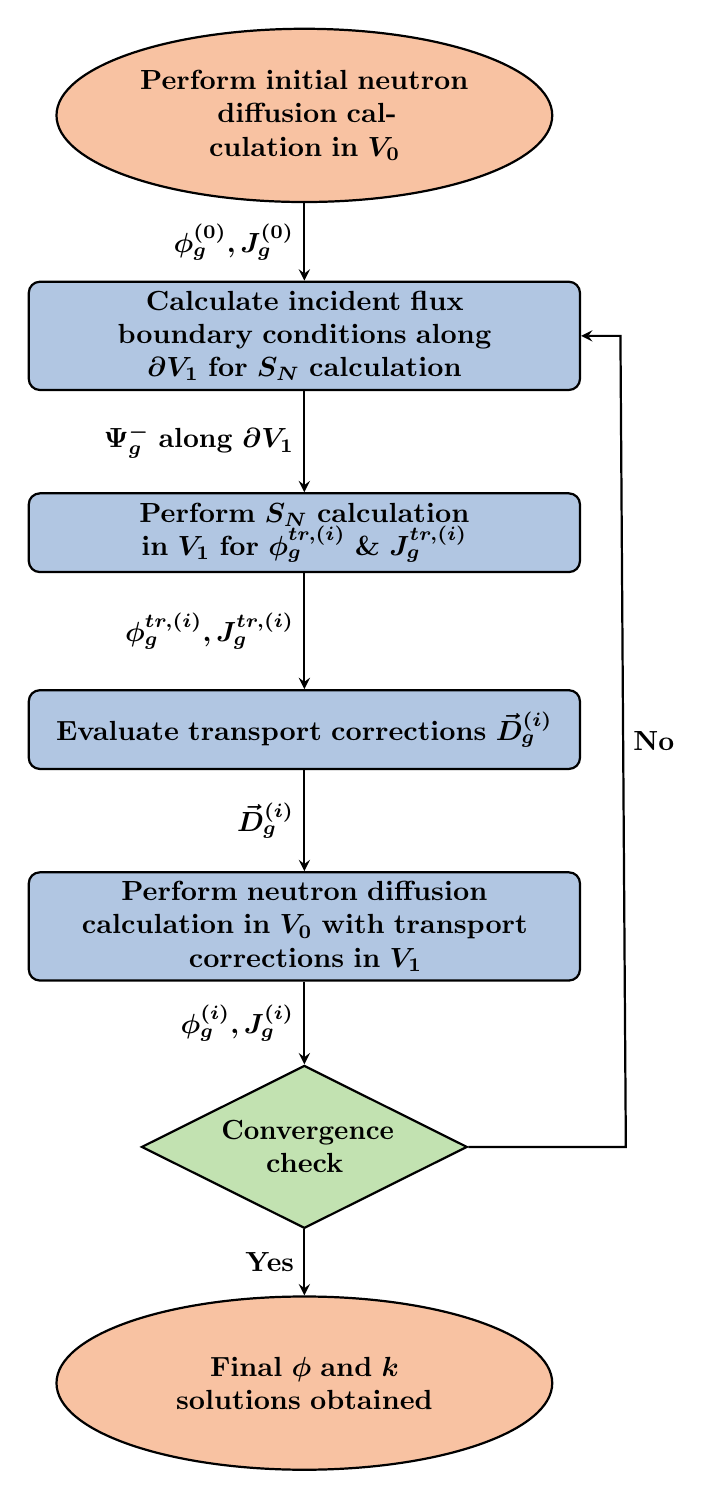
\begin{tikzpicture}
    \node (1) [object] {\textbf{Perform initial neutron\\diffusion calculation in $\bm{V_0}$}};
    \node (2) [process, below of=1, yshift=-1.8cm]
      {\textbf{Calculate incident flux boundary conditions along\\$\bm{\partial V_1}$ for $\bm{S_N}$ calculation}};
    \node (3) [process, below of=2, yshift=-1.5cm]
      {\textbf{Perform $\bm{S_N}$ calculation\\in $\bm{V_1}$ for $\bm{\phi^{tr,(i)}_g}$ \& $\bm{J^{tr,(i)}_g}$}};
    \node (4) [process, below of=3, yshift=-1.5cm]
      {\textbf{Evaluate transport corrections $\bm{\vec{D}^{(i)}_g}$}};
    \node (5) [process, below of=4, yshift = -1.5cm]
      {\textbf{Perform neutron diffusion\\calculation in $\bm{V_0}$ with transport\\corrections in $\bm{V_1}$}};
    \node (6) [decision, below of=5, yshift = -1.8cm]
      {\textbf{Convergence\\check}};
    \node (7) [object, below of=6, yshift = -2cm]
      {\textbf{Final $\bm{\phi}$ and $\bm{k}$\\solutions obtained}};
    \draw [arrow] (1) -- node[anchor=east] {$\bm{\phi^{(0)}_g, J^{(0)}_g}$} (2);
    \draw [arrow] (2) -- node[anchor=east] {$\bm{\Psi^-_g}$ \textbf{along} $\bm{\partial V_1}$} (3);
    \draw [arrow] (3) -- node[anchor=east] {$\bm{\phi^{tr,(i)}_g, J^{tr,(i)}_g}$} (4);
    \draw [arrow] (4) -- node[anchor=east] {$\bm{\vec{D}^{(i)}_g}$} (5);
    \draw [arrow] (5) -- node[anchor=east] {$\bm{\phi^{(i)}_g, J^{(i)}_g}$} (6);
    \draw [arrow] (6) -- node[anchor=east] {\textbf{Yes}} (7);
    \draw [arrow] (6) -- ([shift={(2cm,0cm)}]6.east)-- node[anchor=west] {\textbf{No}} ([shift={(0.5cm,0cm)}]2.east)--(2);
  \end{tikzpicture}
  \caption{Algorithm flowchart for the hybrid $S_N$-diffusion method. $(i)$ denotes the iteration
  index.}
  \label{fig:algorithm}
\end{figure}

\subsection{$S_N$ Subsolver Boundary Conditions} \label{sec:sn-bc}

Convergence of the hybrid $S_N$-diffusion method requires appropriate boundary conditions for
the $S_N$ subproblem.
Given that we want to limit the coverage of $V_1$ to the control rod region and its
immediate vicinity, $V_1$ should be sufficiently smaller than $V_0$, but large enough to capture
anisotropies in the flux due to the control rod. As a consequence, the boundaries $\partial V_1$ 
lie well within $V_0$. We obtain the best estimate for boundary fluxes for the $S_N$ solver by
applying the $P_1$ approximation for evaluating the neutron angular flux along
the discrete ordinates $\hat{\Omega}_d$ of the $S_N$ angular quadrature set as follows
%
\begin{align}
  \Psi_{g,d} &\approx \frac{1}{4\pi}\left(\phi^\text{diff}_g+3\hat{\Omega}_d\cdot
  \vec{J}^\text{diff}_g\right) \nonumber \\
  &=\frac{1}{4\pi}\left(\phi^\text{diff}_g-3\hat{\Omega}_d\cdot D_g\nabla\phi^\text{diff}_g\right)
\end{align}
%
where the diff superscript denotes flux estimates from the latest neutron diffusion calculation.
With this relation, we can formulate the boundary source term for the $S_N$ subsolver by setting
the incident boundary flux source,
$\Psi^\text{inc}_{g,d}$, in Eq.\ \ref{eq:boundary-source} to
%
\begin{gather}
  \Psi^\text{inc}_{g,d} = \frac{1}{w}
  \left(\phi^\text{diff}_g-3\hat{\Omega}_d\cdot D_g\nabla\phi^\text{diff}_g\right)
\end{gather}

\subsection{Buffer Region} \label{sec:buffer-region}

The $S_N$ subsolver boundary conditions will generally cause deviations
in the flux and transport correction values since the $P_1$ approximation captures
linear anisotropic flux at best. However, the results of this paper will show that
the influence of boundary conditions on the accuracy of
the transport correction terms does not extend far from the boundary $\partial V_1$ in optically
thick media due to competing influences from the bulk scattering and absorption effects in $V_1$.
Transport correction values ($\vec{D}_g$) generated with the $S_N$ subsolver within $V_1$ are
accurate everywhere up to a few centimeters inside of $V_1$.

For accurate flux estimates with the hybrid method, we propose that $V_1$ must be large enough to
provide accurate transport corrections near the highly-absorbing control rod while simultaneously
accommodating for inaccurate transport correction values near $\partial V_1$. Right before each
neutron diffusion calculation, the solver must determine where the inaccurate transport correction
values occur and discard them. We will refer to the region near $\partial V_1$ in which the
transport correction values are discarded as the \textit{buffer region} ($V_1'$).
$V_1'$ shares the same outer boundary $\partial V_1$ as $V_1$. Consequently, the neutron
diffusion calculation on $V_0$ will only apply transport corrections in $V_1$ excluding $V_1'$.

In this discussion thus far, we have yet to establish the cutoff boundary for $V_1'$ within $V_1$
opposite to $\partial V_1$. A natural/intuitive criterion for the location of the cutoff boundary
would be where the components of the drift correction variable $\vec{D}_g$ become zero (i.e.,
where the components change signs). The reasons for this criterion are twofold. Firstly, at
points where the $\vec{D}_g$ components are zero, the flux is approximately isotropic along the
axes corresponding to the components because value of $\vec{D}_g$ represents how much correction a
standard neutron diffusion model requires. Secondly, this choice preserves the smoothness of the
neutron flux and flux gradient.
%
\begin{figure}[b]
	\centering
	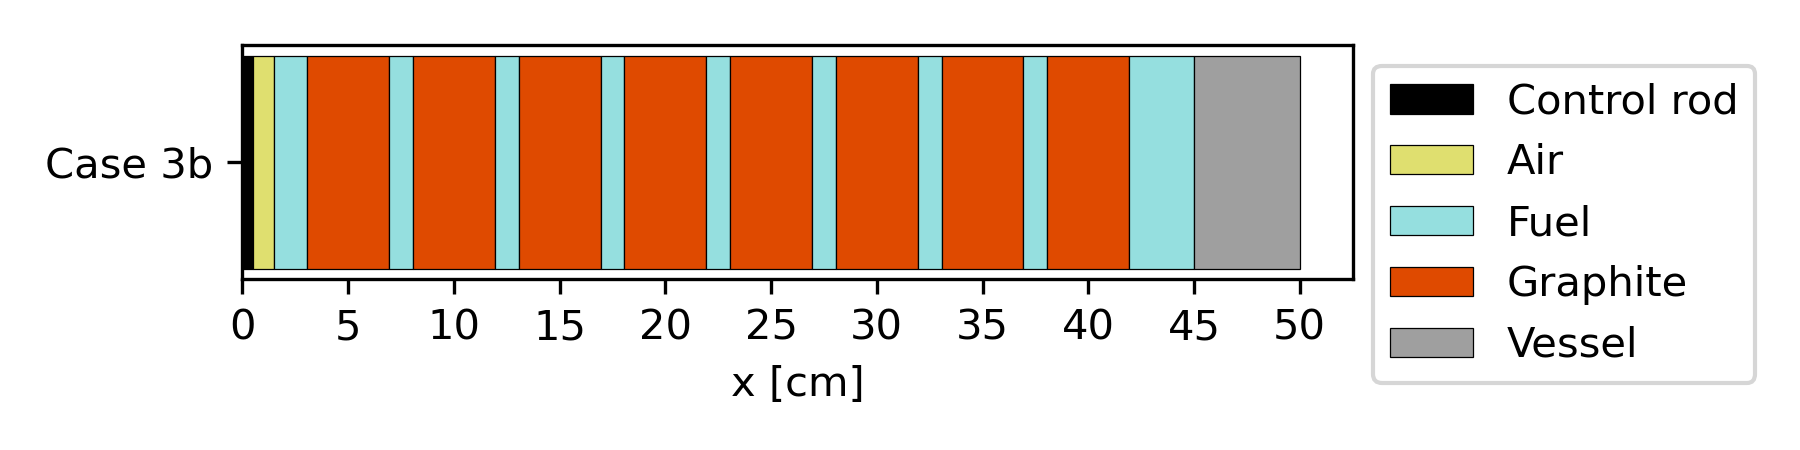
\includegraphics[width=.75\columnwidth]{case-3b-geometry}
	\caption{1-D geometry for Case 3b.}
	\label{fig:3b-geometry}
\end{figure}

Here, we use Case 3b of the 1-D test cases to be covered in Section \ref{sec:msre} to illustrate
the buffer region and the behavior of $\vec{D}_g$. Case 3b is a 1-D heterogeneous slab problem
consisting of control rod, air, fuel-graphite repeating lattice, and reactor vessel regions as
shown in Figure \ref{fig:3b-geometry}. The fuel regions are neutron-multiplying media containing
$^\text{235}$U fissile material. The material compositions of each region are from the \gls{MSRE}
reference design and the start-up fuel composition \cite{fratoni_molten_2020}.
Case 3b has reflecting boundary conditions on the left boundary and vacuum boundary conditions on
the right boundary.
%
\begin{figure}[htb!]
    \centering
    \begin{subfigure}[t]{.49\textwidth}
        \centering
        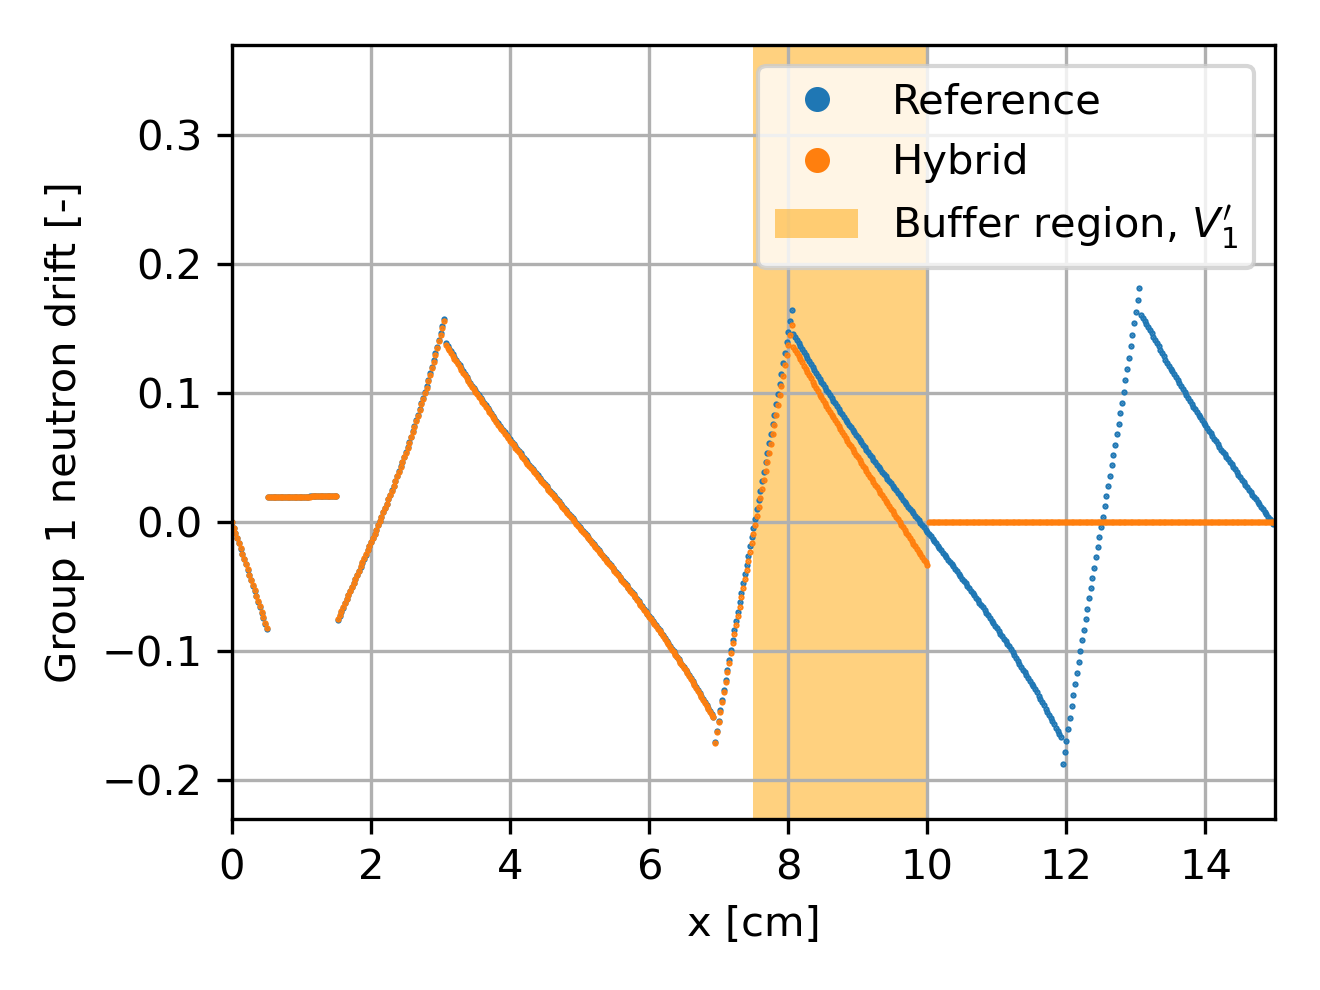
\includegraphics[width=\textwidth]{case-3b-group-1-drift}
    \end{subfigure}
    \hfill
    \begin{subfigure}[t]{.49\textwidth}
        \centering
        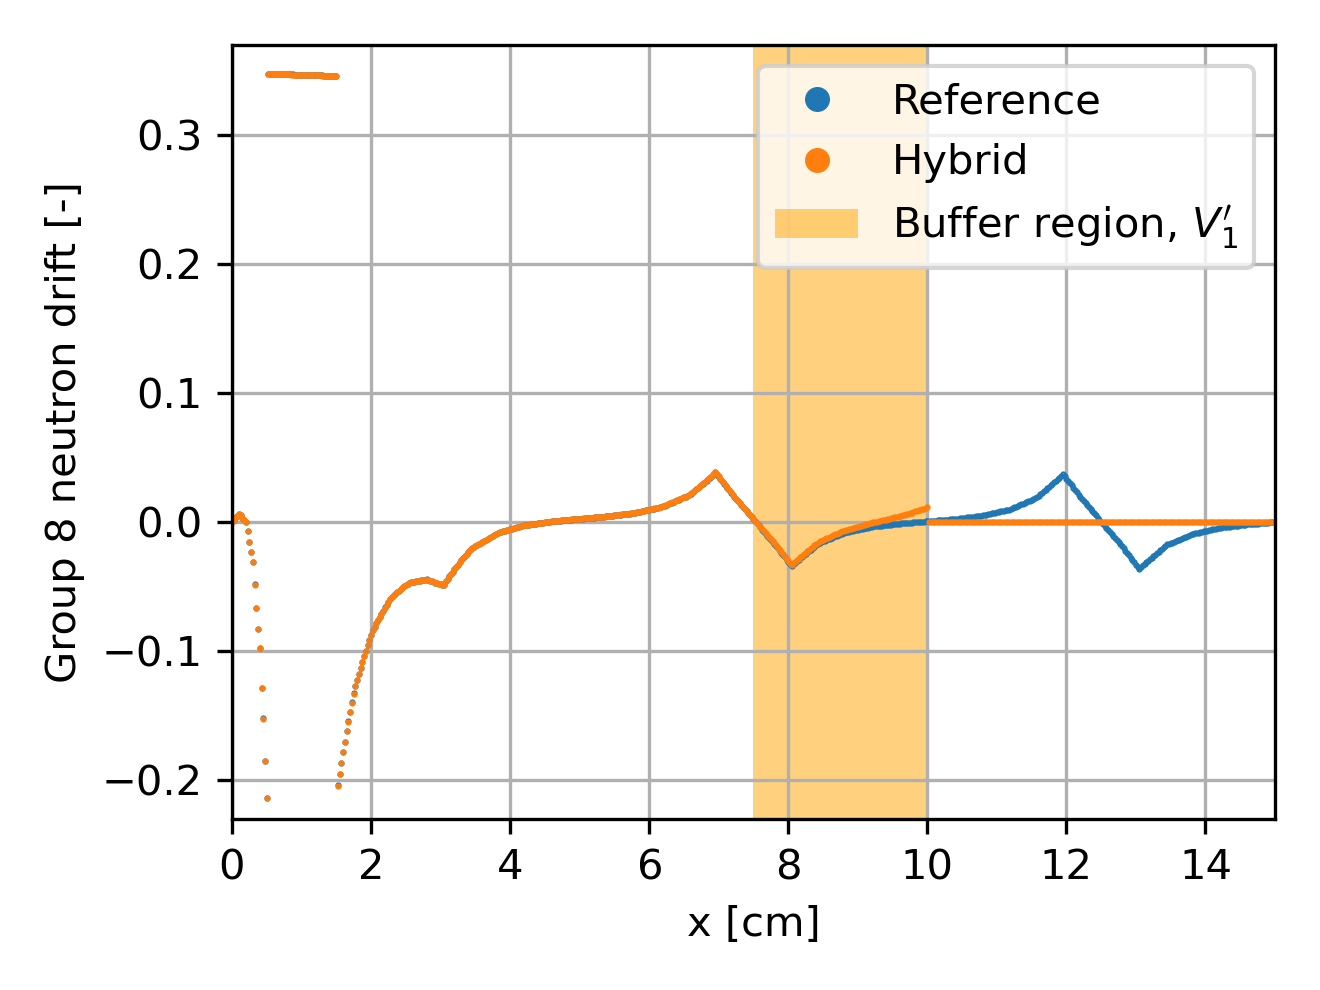
\includegraphics[width=\textwidth]{case-3b-group-8-drift}
    \end{subfigure}
    \caption{The reference and hybrid drift ($\vec{D}_g$) distributions for group 1 and 8 calculated
      from $S_8$ and $S_8$-diffusion simulations. The correction subregion $V_1$ spans $x=0$ cm to
      $x=10$ cm. The buffer region, $V_1'$, is highlighted in yellow.}
    \label{fig:3b-drift-1}
\end{figure}

We ran an eight energy group $S_8$ $k$-eigenvalue simulation with the newly implemented $S_N$ solver
on Moltres to generate reference $\vec{D}_g$ distributions. We also ran an eight-group hybrid
$S_8$-diffusion simulation with the $S_8$ method for generating $\vec{D}_g$ in $V_1$. We set $V_1$
to encompass the control rod region and its vicinity from $x=0$ to $10$ cm based on the geometry in
Figure \ref{fig:3b-geometry}. Figure \ref{fig:3b-drift-1} shows the $\vec{D}_1$ and $\vec{D}_8$
distributions from $x=0$ to $15$ from the reference $S_8$ and hybrid simulations. The hybrid
$\vec{D}_g$ distribution is zero beyond $x=10$ cm because no corrections are generated outside of
$V_1$. Comparing the hybrid distributions to the reference distributions in both energy groups, the
hybrid distributions are accurate up to around $x=8$ cm. Working backward towards the control rod
at $x=0$-$0.5$ cm, the $\vec{D}_g$ values go to zero at $x=7.5$ cm. Therefore, the buffer
region $V_1'$ lies between $x=7.5$ cm and $x=10$ cm. While $V_1$ is pre-determined at the start of
the simulation and fixed for all energy groups, $V_1'$ does not necessarily coincide for all
energy groups and coordinate axes.

\subsection{Numerical Implementation} \label{sec:numerical-implementation}

This section details the numerical implementation of the hybrid $S_N$-diffusion method with
drift correction terms in Moltres.

Moltres \cite{lindsay_moltres_2017} is an open-source multiphysics reactor simulation software
developed for \gls{MSR} analysis. It is built on the \gls{MOOSE} open-source finite-element
framework \cite{giudicelli_30_2024}, which facilitates multiphysics coupling with different
\gls{MOOSE}-based and \gls{MOOSE}-wrapped applications. We implemented the hybrid $S_N$-diffusion
model in Moltres to leverage existing multigroup neutron diffusion modeling capabilities that are
relevant to the newly implemented $S_N$ neutron transport model and the $S_N$-to-diffusion coupling
framework. All source code for the hybrid $S_N$-diffusion model is openly available on the Moltres
GitHub repository\footnote{\url{https://github.com/arfc/moltres/}}.

Moltres presently comes with a Python script for postprocessing and extracting neutron group
constant data from OpenMC \cite{boyd_multigroup_2019} or Serpent 2 \cite{leppanen_serpent_2014}
simulation output files. The script reorganizes the group constant data into a
JSON format file. We introduced new changes to the Python script to extract
the macroscopic total cross sections $\Sigma_{t,g}$ and the higher-order macroscopic Legendre
scattering moments $\Sigma^{g'\rightarrow g}_{s,l}$ for the $S_N$ neutron transport model. A new
\texttt{Material} class called \texttt{MoltresSNMaterial} creates material
property variables for each group constant for the $S_N$ model to read during a neutronics
simulation. If the user provides group constant data at multiple reactor temperature states,
\texttt{MoltresSNMaterial} can interpolate the data to simulate temperature-dependent reactivity
changes.

The new \texttt{MoltresUtils} class contains ``utility'' functions required by the $S_N$ model.
These functions include: a function to retrieve directions and weights defined by a
level-symmetric quadrature set of order $N$, a function to retrieve reflecting directions at
reflecting boundaries, and a function to compute spherical harmonic flux moments for anisotropic
scattering. We pre-computed the direction and weight values for the level-symmetric quadrature sets
using a Python script and hard-coded them in Moltres to reduce computational expense during
simulations.

The \gls{SAAF} $S_N$ method defines $G$ energy groups and $N_d$ discrete directions for a total
of $G\times N_d$ angular flux variables $\Psi_{g,d}$. The Moltres $S_N$ model groups the
$\Psi_{g,d}$ variables by energy group into $G$ array variables. An array variable is a
set of standard field variables to help with dealing with setting up simulations with high
dimensionality. Each standard variable of an array variable is referred to as a component in the
array variable. In this work, we opted for
2nd-order Lagrange shape functions to approximate the $\Psi_{g,d}$ variables in the finite-element
analysis for improved convergence rates in mesh refinement studies over 1st-order shape functions.
All $S_N$ simulations in this work
employ the \gls{PJFNK} solver \cite{knoll_jacobian-free_2004} with HYPRE-BoomerAMG
\cite{hypre_hypre_2022} for preconditioning.

%The terms in the \gls{SAAF} $S_N$ equations
%are represented by kernel and BC classes inheriting from \texttt{ArrayKernel} and
%\texttt{ArrayIntegratedBC} template classes. Table \ref{tab:saaf-sn} lists the class names
%corresponding to each term in Eq.\ \ref{eq:saaf-vt}.
%%
%\begin{table}[htb]
%  \centering
%  \caption{Names of the Kernels and BCs representing the \gls{SAAF} $S_N$ equations.}
%  \begin{tabular}{l l l}
%    \toprule
%    Term name & Class name \\
%    \midrule
%    Time derivative & \texttt{SNTimeDerivative} \\
%    Streaming & \texttt{SNStreaming} \\
%    Collision & \texttt{SNCollision} \\
%    Scattering & \texttt{SNScattering} \\
%    Prompt fission source & \texttt{SNFission} \\
%    Delayed neutron source & \texttt{SNDelayed} \\
%    Vacuum boundary & \texttt{SNVacuumBC} \\
%    Reflecting boundary & \texttt{SNReflectingBC} \\
%    Hybrid method boundary source & \texttt{SNDiffusionBC} \\
%    \bottomrule
%  \end{tabular}
%  \label{tab:saaf-sn}
%\end{table}

%The \gls{MOOSE} framework leverages the Eigen \cite{guennebaud_eigen_2010} C++ template library for
%linear algebra operations defined in ArrayKernels and ArrayBCs for array variables. The \gls{SAAF}
%$S_N$ C++ classes contain functions for computing the residual and Jacobian contributions
%of each term. The \gls{FEM} numerical solver deems to have reached a converged solution if the sum
%of residual contributions falls below a defined tolerance value.

Moltres initializes the drift correction variables $\vec{D}_g$ as auxiliary array variables
with three components corresponding to their $x$, $y$, and $z$ components. Auxiliary variables
encompass all field variables which are not directly determined during the \gls{PJFNK}
calculation stage. The drift and boundary correction variables are computed during the
post-calculation stages using $\Psi_{g,d}$.
New kernel classes, \texttt{GroupDrift} and \texttt{VacuumCorrectionBC}, add
drift and boundary correction terms to the transport-corrected neutron diffusion solver.

The hybrid method employs the \texttt{MultiApp} system \cite{gaston_physics-based_2015} to
implement the fixed point iterative coupling between the $S_N$ and neutron diffusion solvers for
the hybrid $S_N$-diffusion method.
The \texttt{MultiApps} and \texttt{Transfers} systems from \gls{MOOSE} provide flexible interfaces
for setting up iterative solvers and transferring data between the solvers.
Excluding the initial neutron diffusion calculation,
each outer (fixed point) iteration comprises of an inner $S_N$ calculation on the correction
subregion and an inner neutron diffusion calculation on the entire domain. The \gls{FEM} algorithm
in Moltres determines an individual solver reaches convergence when the combined
residual contributions fall below a specified convergence tolerance threshold. The fixed point
iteration scheme in the \texttt{MultiApps} system for coupling multiple individual
solvers (referred to as apps) requires users to specify a main app for the final convergence check
after each outer iteration to terminate the iterations. The scheme also requires users to set a
fixed point convergence tolerance value independent of the tolerance values of each individual
solver. Naturally, the fixed point tolerance value must be equal to or greater than the tolerance
value of the main individual solver for the possibility of overall convergence. The hybrid method
implementation in Moltres sets the neutron diffusion solver as the main app and the $S_N$ subsolver
as the sub app.

%\subsection{Summary} \label{sec:hybrid-summary}
%
%The hybrid $S_N$-diffusion method improves on the standard neutron
%diffusion method by iteratively applying transport corrections generated from solving the $S_N$
%neutron transport
%method in subdomains containing highly neutron-absorbing regions (e.g., control rods). By limiting
%the size of the subdomain in which $S_N$ subsolver is active, the hybrid method saves on
%computational expense at the cost of some accuracy in the regions not treated with transport
%corrections. In turn, the neutron diffusion subsolver provides approximate boundary source terms
%for the $S_N$ subsolver boundary conditions. 
%
%I presented two different formulations of transport correction that I investigated in this work for
%implementation in the hybrid method: diffusion correction and drift correction schemes. Diffusion
%correction involves replacing the diffusion coefficient in the neutron diffusion equations with
%corrected coefficients derived from neutron transport methods. Drift correction involves
%introducing additional drift terms to the neutron diffusion equations to provide transport
%corrections. I found drift correction to be more promising due to issues with division by zero when
%obtaining diffusion corrections.
%
%In my investigations with the hybrid method, I found that the $S_N$ subsolver produces
%accurate transport correction values in most of the subdomain. However, the transport correction
%values near the $S_N$ subsolver boundary are inaccurate due to the approximate boundary conditions
%provided by the diffusion subsolver. Thus, I developed an adaptive boundary algorithm that
%establishes a buffer region in which transport correction parameters are discarded to improve
%$S_N$-diffusion coupling and preserve smoothness of the neutron flux gradients. The algorithm
%operates independently in each neutron energy group since the buffer region cutoffs
%do not necessarily coincide for all energy groups. The
%correction region is pre-determined at the start of the simulation, thus requiring preliminary
%analysis by the user to confirm that the region size is appropriate for the problem.
%
%By implementing the hybrid method in Moltres, I leveraged existing neutronics modelling
%capabilities and parallel numerical solver libraries available through Moltres and \gls{MOOSE} to
%enable full-core, time-dependent reactor simulations on \gls{HPC} clusters.
%In the next chapter, I verify the hybrid method with both diffusion and drift correction schemes
%against Monte Carlo and $S_N$ neutron transport
%methods through various neutronics test cases and discuss some significant observations made in my
%investigations.

\section{Numerical Results \& Discussion} \label{sec:msre}

This section demonstrates the hybrid method through 1-D and 2-D $k$-eigenvalue
simulations of the \gls{MSRE}. This work employs the OpenMC Monte Carlo neutral
particle transport software \cite{romano_openmc:_2015} to generate group constants for the hybrid
method and to generate reference solutions for method verification.
The 1-D models serve to verify the newly-implemented $S_N$ and hybrid methods
and to analyze the impact of key input parameters on the hybrid method. The
2-D models test the hybrid method performance through increased spatial dimensionality and
geometric asymmetry relative to the 1-D models. Parametric studies using 2-D models on the $S_N$ angular
discretization reveal its impact on the neutron flux distributions and $k_\text{eff}$.
%Lastly, the 3-D models serve as neutronics model
%validation against the \gls{MSRE} benchmark model by Fratoni et al.\ \cite{fratoni_molten_2020}.
%This section also investigates the computational performance of 3-D simulations on a \gls{HPC}
%cluster.

%Section \ref{sec:msre-gc} details the OpenMC model setup for group constant generation. Section
%\ref{sec:nts-methods} describes and labels the different neutronics methods employed for the
%$k$-eigenvalue simulations. Section \ref{sec:test-metrics} details test metrics relevant to
%neutronics verification and validation. Sections \ref{sec:1d-results}, \ref{sec:2d-results}, and
%\ref{sec:3d-results} discuss the model setups, results, and discussions for the 1-D, 2-D, and 3-D
%\gls{MSRE} models, respectively.


%\section{Test Metrics} \label{sec:test-metrics}
%
%This section defines several metrics for comparing simulation results among the various
%neutronics methods.
%For steady-state eigenvalue calculations, all solvers directly provide the effective neutron
%multiplication factor ($k_\text{eff}$), the rate of neutron population increase between successive
%neutron generations. Reactivity is defined as
%%
%\begin{gather}
%  \rho \equiv \frac{k_\text{eff}-1}{k_\text{eff}}.
%\end{gather}
%%
%Differences in reactivity, for either comparisons between neutronics methods or control rod worth
%calculations, can be calculated as
%%
%\begin{gather}
%  \Delta\rho_{1,2} = \rho_1 - \rho_2 =
%  \frac{k_{\text{eff},1}-k_{\text{eff},2}}{k_{\text{eff},1}k_{\text{eff},2}}.
%\end{gather}
%
%Spatially dependent variables (e.g., neutron group flux, neutron drift) are sampled at fixed 0.1 cm
%intervals along the specified lines (e.g., horizontal, diagonal, etc.) regardless of the actual
%mesh resolution.

\subsection{Neutronics Modeling Setup}

\subsubsection{Group Constant Data Generation on OpenMC} \label{sec:msre-gc}

Deterministic neutron diffusion and $S_N$ neutron transport methods require group constant data in
the form of group-averaged macroscopic neutron cross sections, neutron speeds, and delayed neutron
precursor data.
All simulations in this work used 2nd-order-accurate scattering cross sections approximated using
Legendre polynomials.
%Group constants relevant to the neutron diffusion, $S_N$ neutron transport, or both
%methods in Moltres are:
%%
%\begin{align*}
%  \Sigma_{t,g}=& \mbox{ Macroscopic total cross section in group $g$,} &\\
%  \Sigma_{r,g}=& \mbox{ Macroscopic removal cross section in group $g$,} &\\
%  \Sigma_s^{g'\rightarrow g}=& \mbox{ Macroscopic group-to-group scattering cross section matrix,} &\\
%  \Sigma_{s,l}^{g'\rightarrow g}=& \mbox{ $l$-th Legendre moment of the macroscopic
%        group-to-group scattering} & \\
%                           & \mbox{cross section matrix,} &\\
%  \Sigma_{sp,l}^{g'\rightarrow g}=& \mbox{ $l$-th Legendre moment of the macroscopic
%  group-to-group scattering production} & \\
%                                        & \mbox{cross section matrix,} &\\
%  D_g=& \mbox{ $P_1$-based diffusion coefficient in group $g$,} &\\
%  \nu\Sigma_{f,g}=& \mbox{ Product of the average number of neutrons produced per fission and} &\\
%                  &\mbox{the macroscopic fission cross section in group $g$,}&\\
%  \chi_g=& \mbox{ Neutron fission spectrum in group $g$.}&\\
%\end{align*}
%
%OpenMC generates these group constants using its multigroup cross section generation capability
%\cite{boyd_multigroup_2019}. A group constant postprocessing script for Moltres
%(\texttt{moltres\_xs.py}) parses OpenMC simulation output files and rewrites the group constant
%data into a JSON format file suitable for Moltres simulations. While OpenMC provides most of the
%group constants directly, the postprocessing script calculates $\Sigma_{r,g}$ as
%%
%\begin{align}
%  \Sigma_{r,g} =& \sum^G_{g'\neq g}\Sigma_s^{g\rightarrow g'}+\Sigma_{a,g}-\left(\Sigma_{sp}^{g
%    \rightarrow g} - \Sigma_s^{g\rightarrow g}\right)
%  \shortintertext{where}
%      \Sigma_{a,g} =& \mbox{ macroscopic absorption cross section in group $g$,} \nonumber \\
%      \Sigma_{sp}^{g\rightarrow g} =& \mbox{ macroscopic scattering production cross section from
%      group $g$ to $g$.} \nonumber
%\end{align}
%%
%$\Sigma_{r,g}$ primarily represents the loss of neutrons from group $g$ through outscattering and
%absorption. $\Sigma_{sp}^{g\rightarrow g}$ incorporates neutron multiplication effects from neutron
%knockout reactions into the scattering cross section. Neutronics codes commonly identify neutron
%knockout reactions as scattering reactions, but $\Sigma_{r,g}$ is a convenient parameter in which
%to incorporate neutron knockout effects in the neutron diffusion method.

%OpenMC uses the $P_1$ flux-limited formulation \cite{pomraning_flux-limited_1984} by default for
%calculating $D_g$ as follows
%%
%\begin{align}
%  D_g =& \frac{1}{3\Sigma_{tr,g}},
%  \shortintertext{where}
%  \Sigma_{tr,g} =& \frac{\langle\Sigma_{t,g}\phi_g\rangle-\langle\Sigma_{s1,g}\phi_g\rangle}
%  {\langle\phi_g\rangle}, \nonumber \\
%  \langle\Sigma_{t,g}\phi_g\rangle =& \int_{r\in V}dr \int_{4\pi}d\Omega\int^{E_{g-1}}_{E_g}dE\
%  \Sigma_{t,g}(r,E)\Psi(r,E,\Omega), \nonumber \\
%  \langle\Sigma_{s1,g}\phi_g\rangle =& \int_{r\in V}dr \int_{4\pi}d\Omega\int^{E_{g-1}}_{E_g}dE
%  \int_{4\pi}d\Omega'\int^{\infty}_0dE'\int^1_{-1}d\mu\ \mu\Sigma_s(r,E'\rightarrow E,\Omega'\cdot
%  \Omega)\phi(r,E',\Omega'), \nonumber \\
%  \langle \phi \rangle =& \int_{r\in V}dr\int_{4\pi}d\Omega\int^{E_{g-1}}_{E_g}dE\ \Psi(r,E,\Omega)
%  .\nonumber
%\end{align}

All \gls{MSRE} neutronics simulations ran with the eight neutron energy group structure developed
by Jaradat for \gls{MSRE} analysis \cite{jaradat_development_2021-1}.
Table \ref{table:energy-group} shows the upper neutron energy bounds of the eight-group structure.
This choice balances accuracy and computational expense most appropriately for this work when
compared to other various group structures investigated by Jaradat ranging from four to sixteen
groups.

\begin{table}[htb]
  \centering
  \caption{Neutron energy group structure in this work. Originally devised by Jaradat
  \cite{jaradat_development_2021-1}.}
  \begin{tabular}{r S}
    \toprule
    Group & {Upper energy bound [eV]} \\
    \midrule
    1 & 2.000$\times 10^7$ \\
    2 & 1.353$\times 10^6$ \\
    3 & 6.734$\times 10^4$ \\
    4 & 9.118$\times 10^3$ \\
    5 & 1.487$\times 10^2$ \\
    6 & 4.000$\times 10^0$ \\
    7 & 6.250$\times 10^{-1}$ \\
    8 & 8.000$\times 10^{-2}$ \\
    \bottomrule
  \end{tabular}
  \label{table:energy-group}
\end{table}

Material compositions and densities of all components in the \gls{MSRE} models are from reference
\gls{MSRE} specifications \cite{robertson_msre_1965, fratoni_molten_2020}.
All OpenMC simulations in this work used the ENDF/B-VII.1 nuclear data library
\cite{chadwick_endf/b-vii.1_2011}. All models have a uniform
temperature of 900 K unless otherwise stated. Sections \ref{sec:1d-model-setup} and
\ref{sec:2d-model-setup} provide detailed information pertaining
specifically to the 1-D and 2-D model geometries, respectively.

\subsubsection{Neutronics Methods} \label{sec:nts-methods}

Besides generating group constants for the deterministic methods, OpenMC also provides reference
netruon flux and $k_\text{eff}$ values for all studied cases. OpenMC can run in continuous-energy
(OpenMC-CE) and multigroup (OpenMC-MG) modes. Table
\ref{table:var} details how OpenMC and the deterministic methods represent the position, direction
of travel, neutron energy, and angle-dependence in $\Sigma_s$. The hybrid $S_N$-diffusion method
features representations from either $S_N$ or neutron diffusion depending on the subregion under
consideration. Comparing OpenMC-MG results with OpenMC-CE results allows us
to quantify errors arising from neutron energy group discretization and the 2nd-order scattering
cross section approximations.

\begin{table}[htb!]
  \centering
  \footnotesize
  \caption{Variable representations in OpenMC under continuous-energy (OpenMC-CE) and multigroup
  (OpenMC-MG) modes, and in the $S_N$ neutron transport and neutron diffusion.}
  \begin{tabular}{l l l l l}
    \toprule
    Variable & OpenMC-CE & OpenMC-MG & $S_N$ Transport & Diffusion \\
    \midrule
    Position, $\bm{r}$ & Continuous & Continuous & Discrete & Discrete \\
    Direction of travel, $\bm{\hat{\Omega}}$ & Continuous & Continuous & Discrete & N/A \\
    Energy, $E$ & Continuous & Discrete & Discrete & Discrete \\
    Angle resolution in $\Sigma_s$ & Continuous & $L=2$ & $L=2$ & N/A \\
    \bottomrule
  \end{tabular}
  \label{table:var}
\end{table}

\subsection{1-D Neutronics Models \& Results} \label{sec:1d-results}

%This section presents the models, results, and discussion for the 1-D test cases. Section
%\ref{sec:1d-model-setup} describes the model setup and geometries of the 1-D test cases.
%Section \ref{sec:1d-mesh-conv} discusses the 1-D mesh convergence tests. Lastly, Section
%\ref{sec:1d-results-sub} shows the results and discussion of the 1-D test cases.

\subsubsection{1-D Neutronics Model Setup \& Geometries} \label{sec:1d-model-setup}

This section covers six 1-D test cases with increasing complexity to verify the $S_N$ and hybrid
$S_N$-diffusion implementations and to test the performance of the hybrid
method in response to various geometrical features. The last two cases resemble the
reference \gls{MSRE} design \cite{robertson_msre_1965}, which has centrally located control rods
and air-filled rod guide tubes. Figure \ref{fig:case-geom} shows the geometries of Cases 1a to
3b. All geometries have reflective boundary conditions at $x=0$ cm, thereby
forming half-core or repeating unit cell models. Cases 1a and 1b are repeating unit
cell models with reflecting boundaries on the right-side boundaries to serve as reference cases for
the base-line $S_N$ and neutron diffuson methods. Cases 2a, 2b, 3a, and 3b
are 1-D half-core models with vacuum boundaries on the right-side boundaries.

\begin{figure}[htb!]
  \centering
  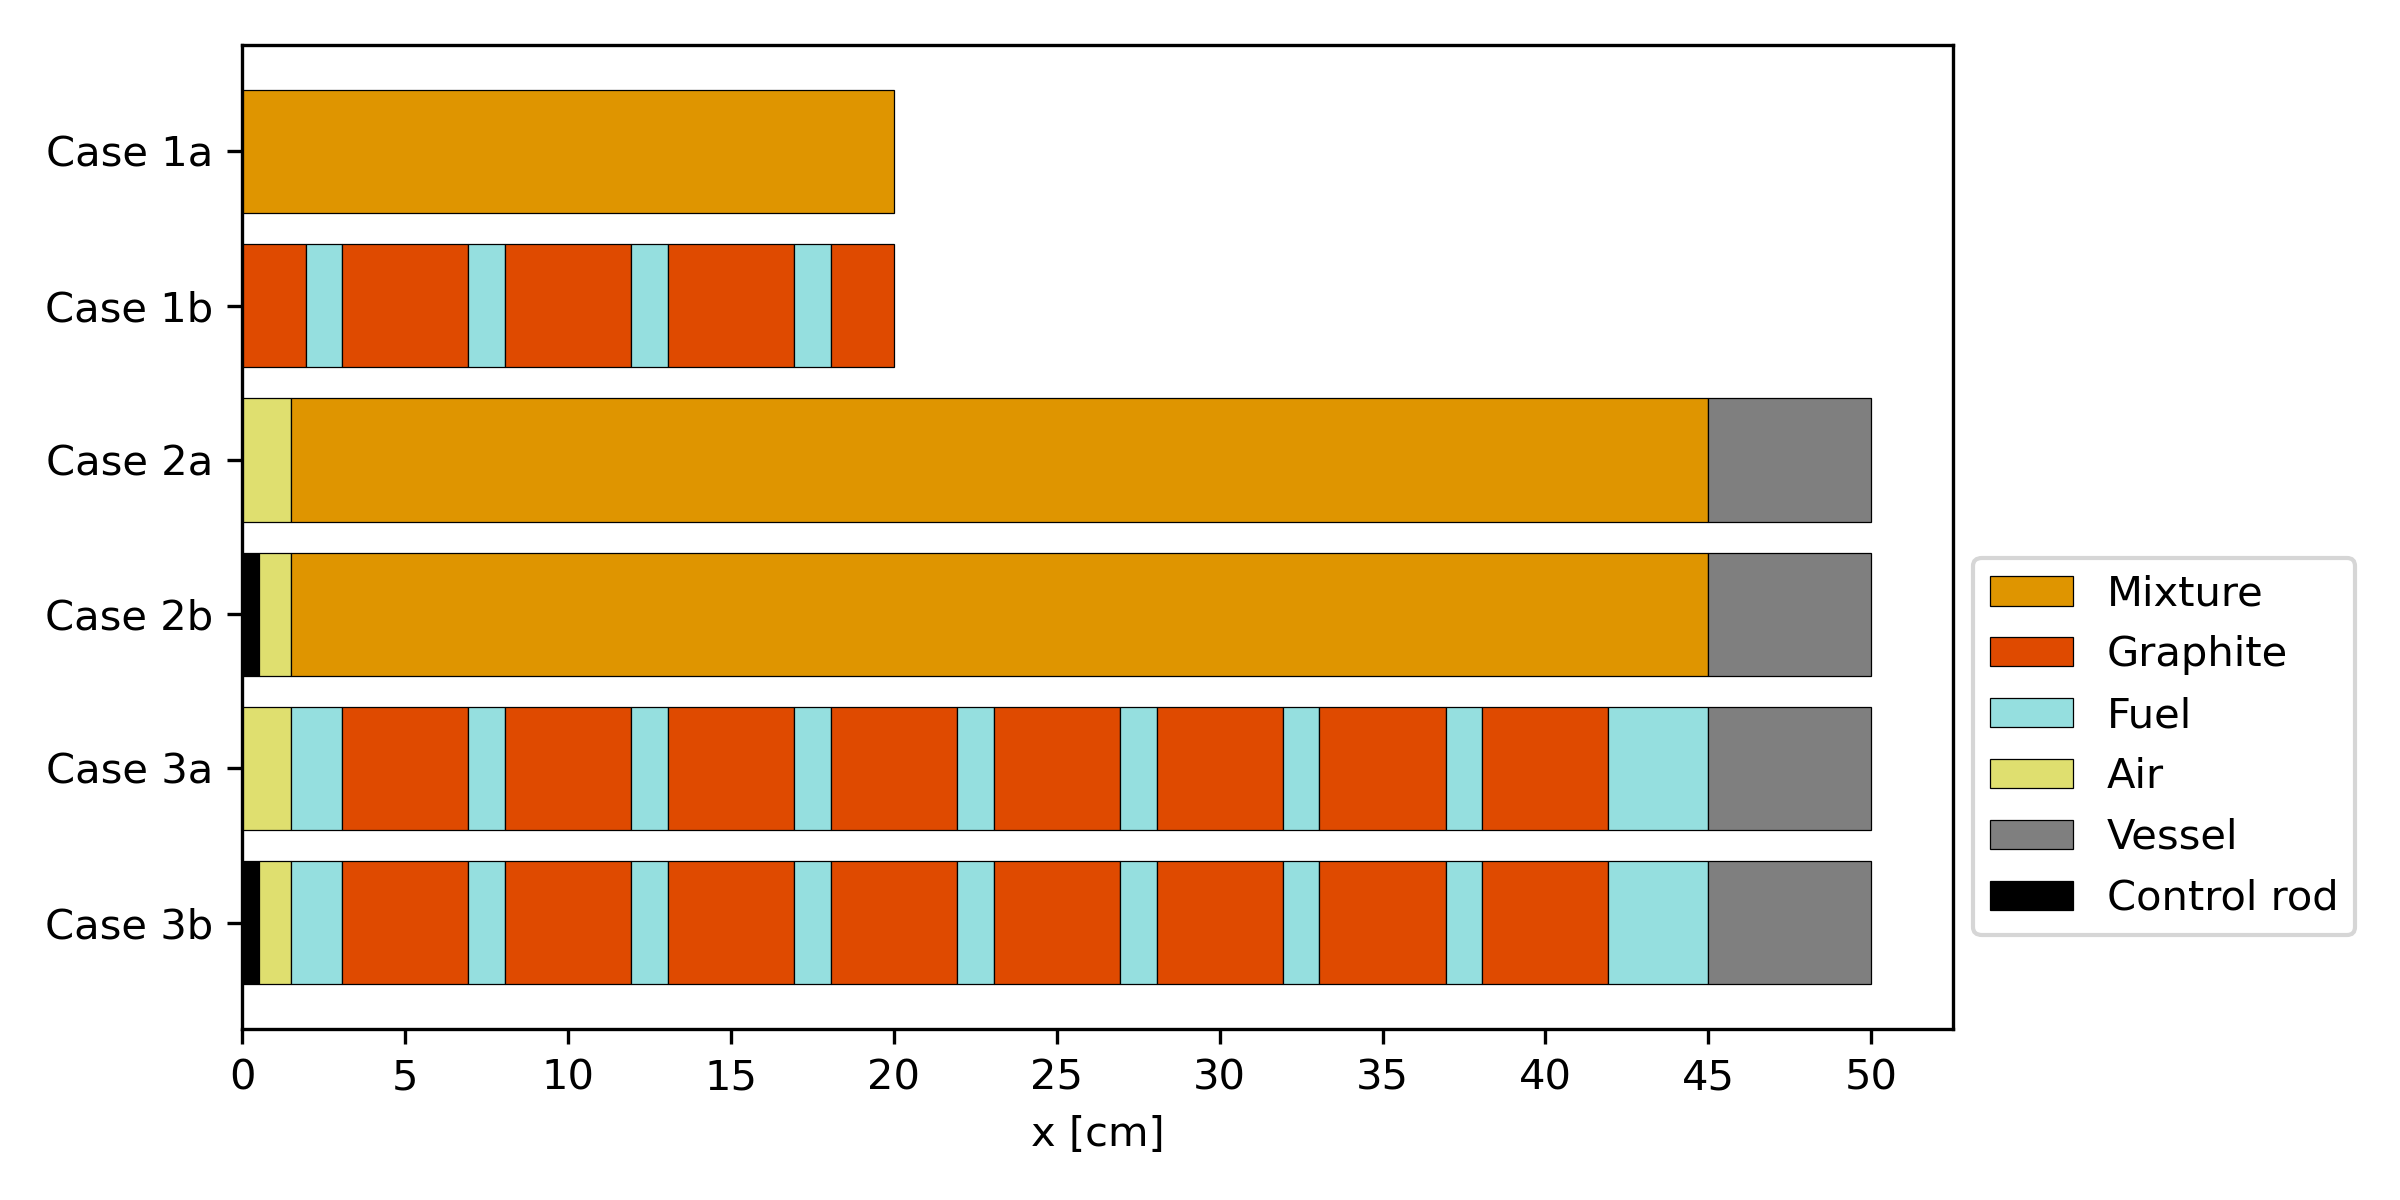
\includegraphics[width=0.8\columnwidth]{case-geometry}
  \caption{Geometries of the 1-D test cases. The material labeled ``mixture'' represents a
    homogeneous mixture of fuel and graphite at a ratio of 22.5\%-77.5\% by volume. All geometries
    have reflective boundary conditions on the boundary at $x=0$ cm. The right-side boundaries are
    reflective for Cases 1a and 1b, and vacuum for Cases 2a, 2b, 3a, and 3b.}
  \label{fig:case-geom}
\end{figure}

%Cases 1a and 1b are simple test cases containing neutron multiplying regions. Cases 1a and 1b serve
%to verify basic neutronics phenomena modeling (e.g., fission, scattering, absorption) of the newly
%implemented $S_N$ and neutron diffusion methods in Python and $S_N$ method in Moltres. I did not
%apply the hybrid method on these cases. Cases 2a and 2b represent 1-D models of the \gls{MSRE} with
%air-filled control rod guide tube regions, a homogenized fuel-graphite lattice regions, and outer
%vessel regions. Case 2b additionally contains a 0.5cm-thick control rod region to contrast with
%Case 2a for control rod worth calculations. Cases 3a and 3b retain the heterogeneous fuel-graphite
%lattice geometry present in the \gls{MSRE}.

In preliminary investigations, the original control rod material composition
(70 wt\% Gd$_2$O$_3$-30 wt\% Al$_2$O$_3$) led to excessively large control rod worth estimates of
approximately 55000 pcm in the 1-D models, effectively halving the $k_\text{eff}$. The worth
estimates are ten times larger
than the 5500 pcm expected from full rod insertion of all three rods in the actual \gls{MSRE}
\cite{fratoni_molten_2020}. Therefore, the proportion of Gd$_2$O$_3$ was reduced to 0.35 wt\% for a
fairer assessment of rod worth in the 1-D models. This change
brought the new rod worth estimates down to below 20000 pcm.

\subsubsection{1-D Neutronics Model Mesh Convergence Tests} \label{sec:1d-mesh-conv}

This mesh convergence tests were run on Case 3b for the neutron diffusion and $S_N$ neutron
transport methods.
%Table \ref{table:mesh-size} shows the mesh element sizes at mesh refinement
%level 0.
Mesh element sizes approximately halve with each successive refinement level up to level 4.
Figures \ref{fig:diff-mesh-k} and \ref{fig:sn-mesh-k} show the convergence of $k_\text{eff}$
estimates observed for Case 3b simulations with neutron diffusion and $S_8$ neutron transport
methods. The $k_\text{eff}$ values plateau at 0.97132 and 0.98138 for the neutron diffusion and
$S_8$ methods, respectively. After two rounds of mesh refinements, both methods fall within
$5\times 10^{-7}$ range of the reference $k_\text{eff}$ values, below the 0.1 pcm ($10^{-5}$)
tolerance value for determining solution convergence.

%\begin{table}[t]
%  \centering
%  \caption{Mesh element sizes at mesh refinement level 0.}
%  \begin{tabular}{l S}
%    \toprule
%    Region & {Mesh size [cm]} \\
%    \midrule
%    Control rod (interior) & 0.04 \\
%    Control rod (near interface) & 0.025 \\
%    Air & 0.125 \\
%    Fuel & 0.1875 \\
%    Graphite & 0.19375 \\
%    Vessel & 0.2 \\
%    \bottomrule
%  \end{tabular}
%  \label{table:mesh-size}
%\end{table}

\begin{figure}[t]
  \centering
  \begin{subfigure}[b]{0.48\columnwidth}
    \centering
    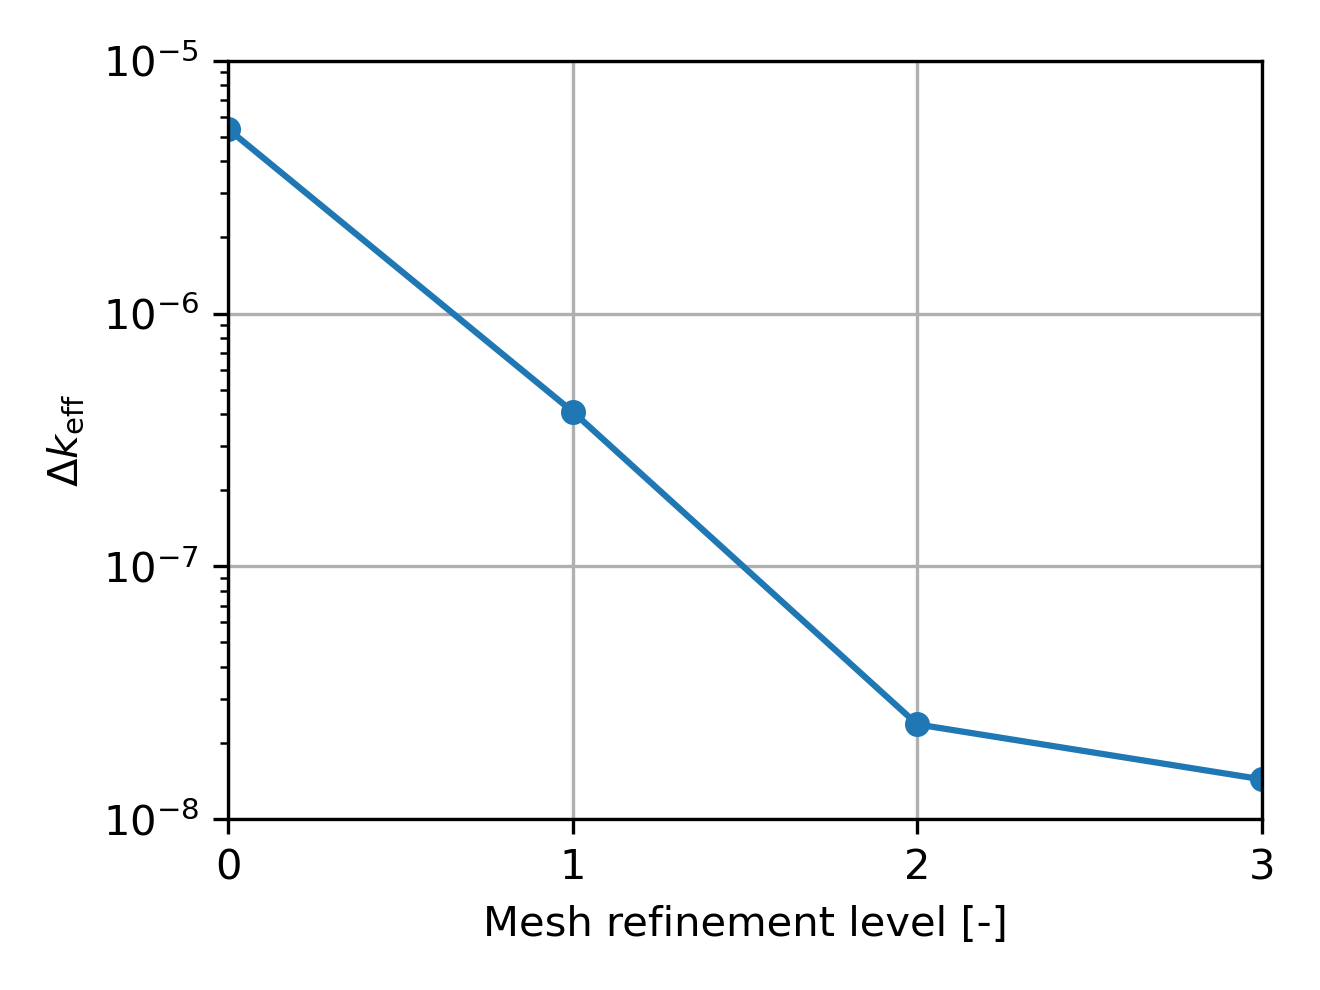
\includegraphics[width=\columnwidth]{diffusion-mesh-convergence-k}
    \caption{Neutron diffusion method}
    \label{fig:diff-mesh-k}
  \end{subfigure}
  \hfill
  \begin{subfigure}[b]{0.48\columnwidth}
    \centering
    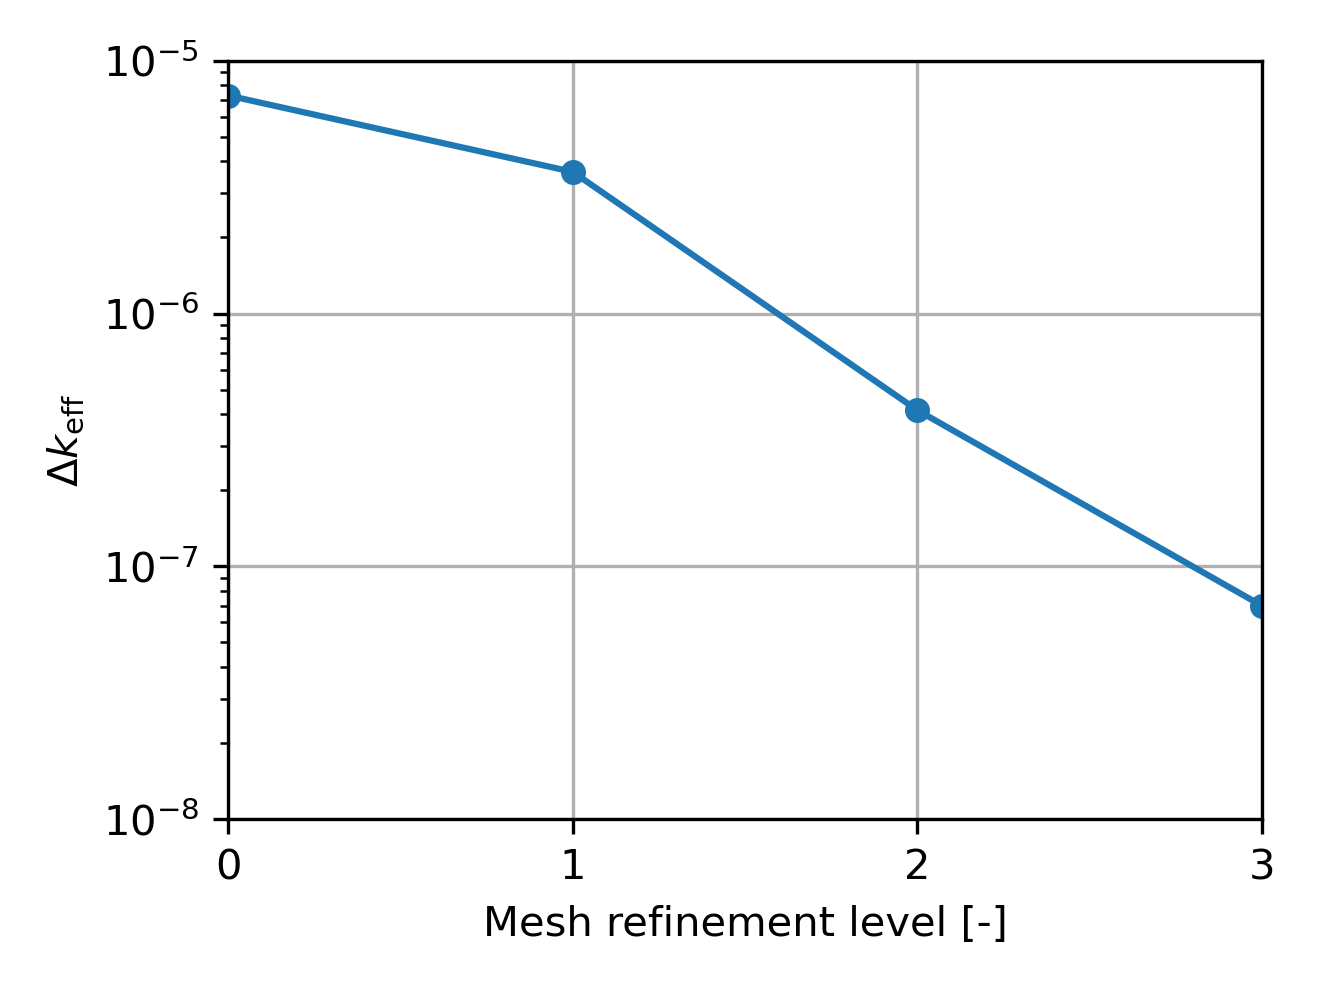
\includegraphics[width=\columnwidth]{sn-mesh-convergence-k}
    \caption{$S_8$ neutron transport method}
    \label{fig:sn-mesh-k}
  \end{subfigure}
  \caption{Convergence of multiplication factor ($k_\text{eff}$) estimates for Case 3b across four
    levels of mesh refinement relative to the finest mesh resolution.}
  \label{fig:mesh-k}
\end{figure}

%Figures \ref{fig:diff-mesh-flux} and \ref{fig:sn-mesh-flux} show the absolute differences in the
%group flux distributions at mesh refinement levels 1 to 3 relative to the reference group flux
%distribution at level 4 (maximum refinement). The plots omit data from level 0 to improve the fidelity
%of the plots as flux differences drop significantly by one order of magnitude with each level of
%refinement.
%These results show that the mesh resolution at level 2 is a sufficient guideline for
%the mesh resolutions used in the subsequent 1-D analyses. Given that the hybrid $S_N$-diffusion
%method comprises of a combination of those
%methods, the hybrid simulations were fully spatially resolved on meshes that are
%appropriately resolved for both neutron diffusion and $S_N$ simulations.
%
%\begin{figure}[htb!]
%  \centering
%  \includegraphics[width=.96\columnwidth]{diffusion-mesh-convergence-flux}
%  \caption{Absolute difference in group fluxes ($\phi_g$) from the neutron diffusion method for
%  mesh refinement levels 1 to 3 relative to the reference group flux distributions at mesh
%  refinement level 4. Flux differences fall by an order of magnitude with each successive mesh
%  refinement.}
%  \label{fig:diff-mesh-flux}
%\end{figure}
%
%\begin{figure}[htb!]
%  \centering
%  \includegraphics[width=.96\columnwidth]{sn-mesh-convergence-flux}
%  \caption{Absolute difference in group fluxes ($\phi_g$) from the $S_8$ neutron transport method
%  for mesh refinement levels 1 to 3 relative to the reference group flux distributions at mesh
%  refinement level 4. Flux differences fall by an order of magnitude with each successive mesh
%  refinement.}
%  \label{fig:sn-mesh-flux}
%\end{figure}

\FloatBarrier

\subsubsection{1-D Numerical Results \& Discussion} \label{sec:1d-results-sub}

%\subsubsubsection{Reactivity}

Figure \ref{fig:1d-rho} shows the difference in reactivities of OpenMC-MG, $S_8$,
neutron diffusion, and hybrid methods relative to OpenMC-CE. The standard deviations of
reactivity values from OpenMC-CE are approximately 40 pcm for Cases 1a and 1b and 60 pcm for the
rest as depicted by the blue highlighted area in Figure \ref{fig:1d-rho}. For Cases 1a and 1b, the
OpenMC-MG, $S_8$, and neutron diffusion methods show excellent agreement with OpenMC-CE as the
reactivity values fall within the one or two standard deviation range. The Case 1 results show
the Moltres and Python implementations are consistent with each other given that they are spatially
well-resolved.

\begin{figure}[htb!]
  \centering
  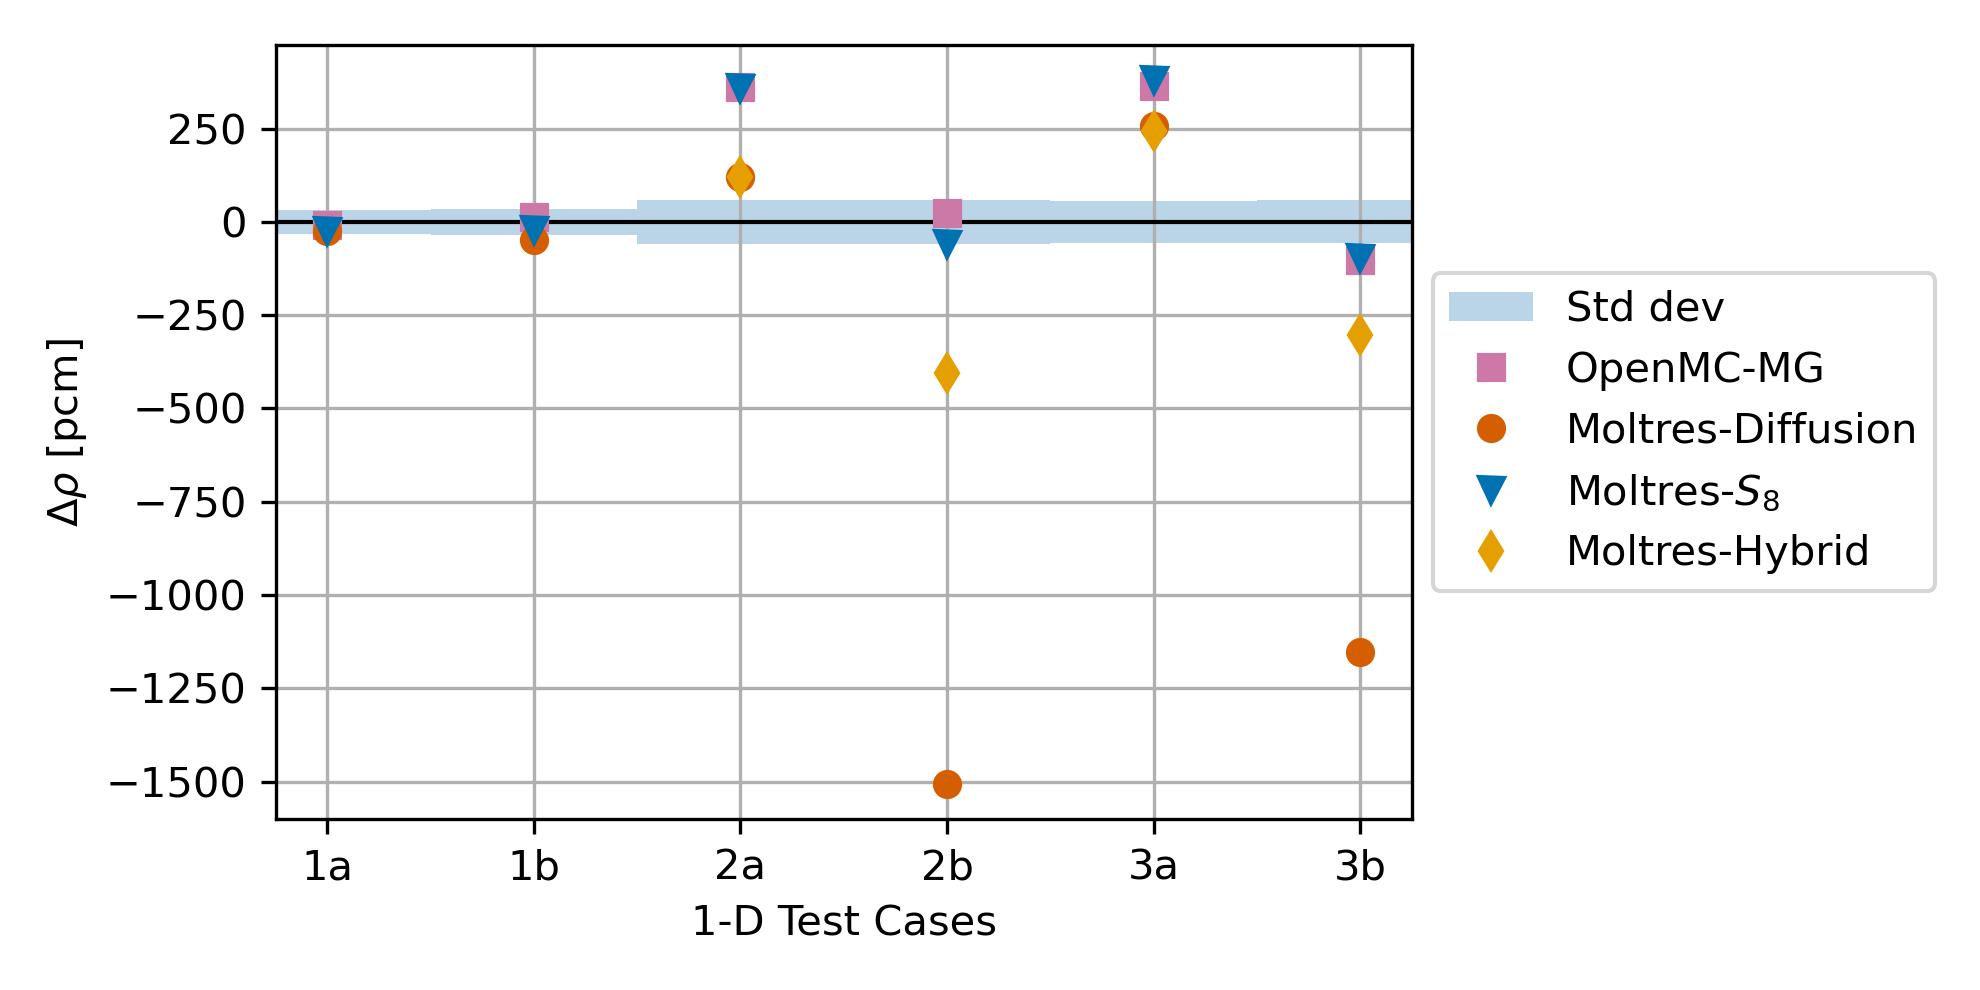
\includegraphics[width=\columnwidth]{rho}
  \caption{Difference in reactivity $\rho$ of all neutronics methods investigated relative
  to OpenMC-CE. The standard deviation refers to the uncertainty associated with the Monte Carlo
  method in OpenMC-CE.}
  \label{fig:1d-rho}
\end{figure}

For all cases, the OpenMC-MG and the $S_8$ methods show consistent agreement with one another. 
While they deviate from OpenMC-CE by approximately 350 pcm for Cases 2a and 3a, they fall within
two standard deviations of OpenMC-CE for Cases 2b and 3b. When increasing the maximum Legendre
polynomial order to approximate the angular dependence in $\Sigma_s^{g'\rightarrow g}$ from
2nd-order to 3rd-order, the reactivity changed by only 1 pcm. Therefore, we attribute the
reactivity discrepancies to the eight neutron energy group structure which remains the
only significant difference between OpenMC-CE and the multigroup methods.

The neutron diffusion and hybrid methods agree closely with one another for Cases 2a and 3a which
exclude the control rod region. This shows that the hybrid method provides similar $k_\text{eff}$
estimates to the neutron diffusion method in 1-D simulations without highly neutron-absorbing
regions. Compared to the OpenMC-MG and $S_8$ reactivity values, the neutron diffusion and hybrid
method reactivity values agree closer with the reference OpenMC-CE value. However, this is likely
due to favorable error cancellation in these lower-fidelity methods. Figure \ref{fig:3a-flux-diff}
shows that the OpenMC-MG and $S_8$ methods reproduce
the OpenMC-CE flux distribution more accurately than the neutron diffusion and hybrid methods.

In Cases 2b and 3b, the neutron diffusion method largely fails to accurately capture the
effect of introducing the control rod region as evidenced by the -1500 pcm and -1150 pcm
discrepancies relative to OpenMC-CE. The hybrid method fares better with -400 pcm and -300 pcm
discrepancies.

%\subsubsubsection{Control rod worth}

Moving the discussion to control rod worths, figure \ref{fig:1d-worth} shows the percentage
difference in rod worths for Cases 2 and 3 of OpenMC-MG, $S_8$, neutron diffusion, and hybrid
methods relative to OpenMC-CE. We calculated the rod worth estimates from each method by taking the
difference in reactivity between the ``rod out'' (a) and ``rod in'' (b) configurations of Cases 2
and 3. All neutronics methods overestimate the rod worth relative to OpenMC-CE, resulting in
positive percentage difference values observed in the figure.
The neutron diffusion methods clearly show up as outliers with rod worth estimates in excess
of 8\%. The remaining methods cluster around 2.5\% and 3\% percentage difference for Cases
2 and 3.

Given that the hybrid method rely on transport corrections derived from the $S_N$ method, the
$S_8$ rod worth estimates serve as the
reference point for hybrid method verification. Additionally, errors arising from the multigroup
approximation affect both hybrid and $S_N$ simulations to similar degrees. Nevertheless, the hybrid
method provides significant improvements in rod worth estimates over the neutron diffusion method.

\begin{figure}[h]
  \centering
  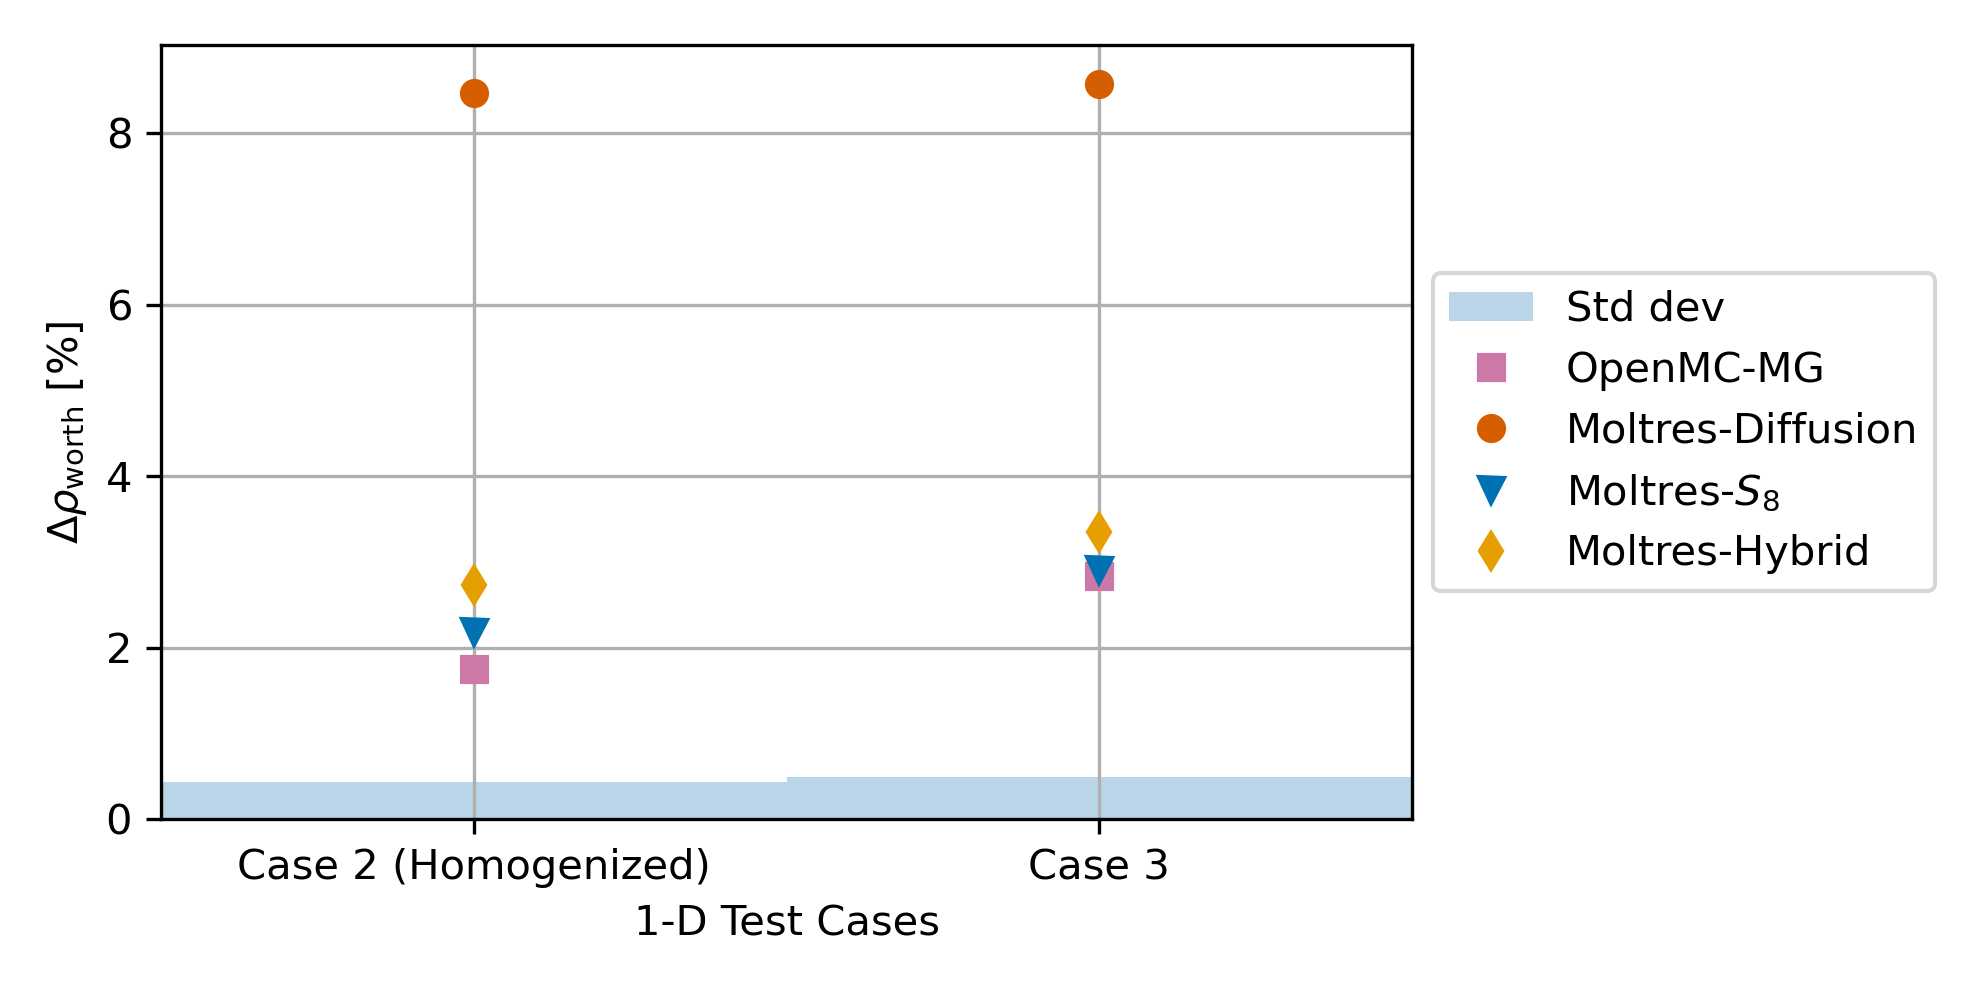
\includegraphics[width=\columnwidth]{worth}
  \caption{Percentage difference in rod worth for Cases 2 and 3 of all neutronics methods
  investigated relative to OpenMC-CE. All percentage difference values are consistently positive.}
  \label{fig:1d-worth}
\end{figure}

%\subsubsubsection{Neutron flux distribution}

The next discussion on the neutron flux distributions focuses on Cases 3a and 3b which most closely
resemble the actual \gls{MSRE} reactor geometry. Cases 3a and 3b resemble the \gls{MSRE} reactor
with a control rod withdrawn and inserted, respectively.
%
%Figures \ref{fig:3a-flux} and
%\ref{fig:3b-flux} show the neutron group flux distributions for Cases 3a and 3b from OpenMC-CE and
%OpenMC-MG. Differences between the two methods arise from the multigroup approximation, notably in
%group 2 for Case 3a and groups 2, 6, 7, 8 for Case 3b. Future work aimed at finding a better
%neutron energy group structure should at minimum focus on improving fidelity in the listed energy
%groups.
%
For a fair evaluation of the deterministic multigroup methods without distortions from the
multigroup approximation, we chose to compare their flux distributions with the OpenMC-MG flux
distribution. Figures \ref{fig:3a-flux-diff} and \ref{fig:3b-flux-diff} show the absolute
difference in neutron group flux distributions of the Moltres-$S_8$, diffusion, and
hybrid methods relative to OpenMC-MG.
The neutron diffusion and hybrid methods fare worse than the $S_8$ method at capturing the
oscillatory pattern in groups 1, 2, 5, 7, and 8 arising from the fuel-graphite lattice geometry
along $x=5$ cm to 10 cm. In both Cases 3a and 3b, the neutron diffusion method (yellow plot lines)
exhibits significant flux deviations in groups 1, 2, 7, and 8 near $x=0$ cm.
The hybrid method
provides significant improvements in neutron flux distributions compared to the neutron diffusion
method as shown by the generally smaller per-group flux deviations particularly near $x=0$ cm.

%\begin{figure}[ht]
%  \centering
%  \includegraphics[width=\columnwidth]{case-3a-flux}
%  \caption{Case 3a neutron group flux distributions from OpenMC-CE and OpenMC-MG.}
%  \label{fig:3a-flux}
%\end{figure}
%
%\begin{figure}[ht]
%  \centering
%  \includegraphics[width=\columnwidth]{case-3b-flux}
%  \caption{Case 3b neutron group flux distributions from OpenMC-CE and OpenMC-MG.}
%  \label{fig:3b-flux}
%\end{figure}

\begin{figure}[p]
  \centering
  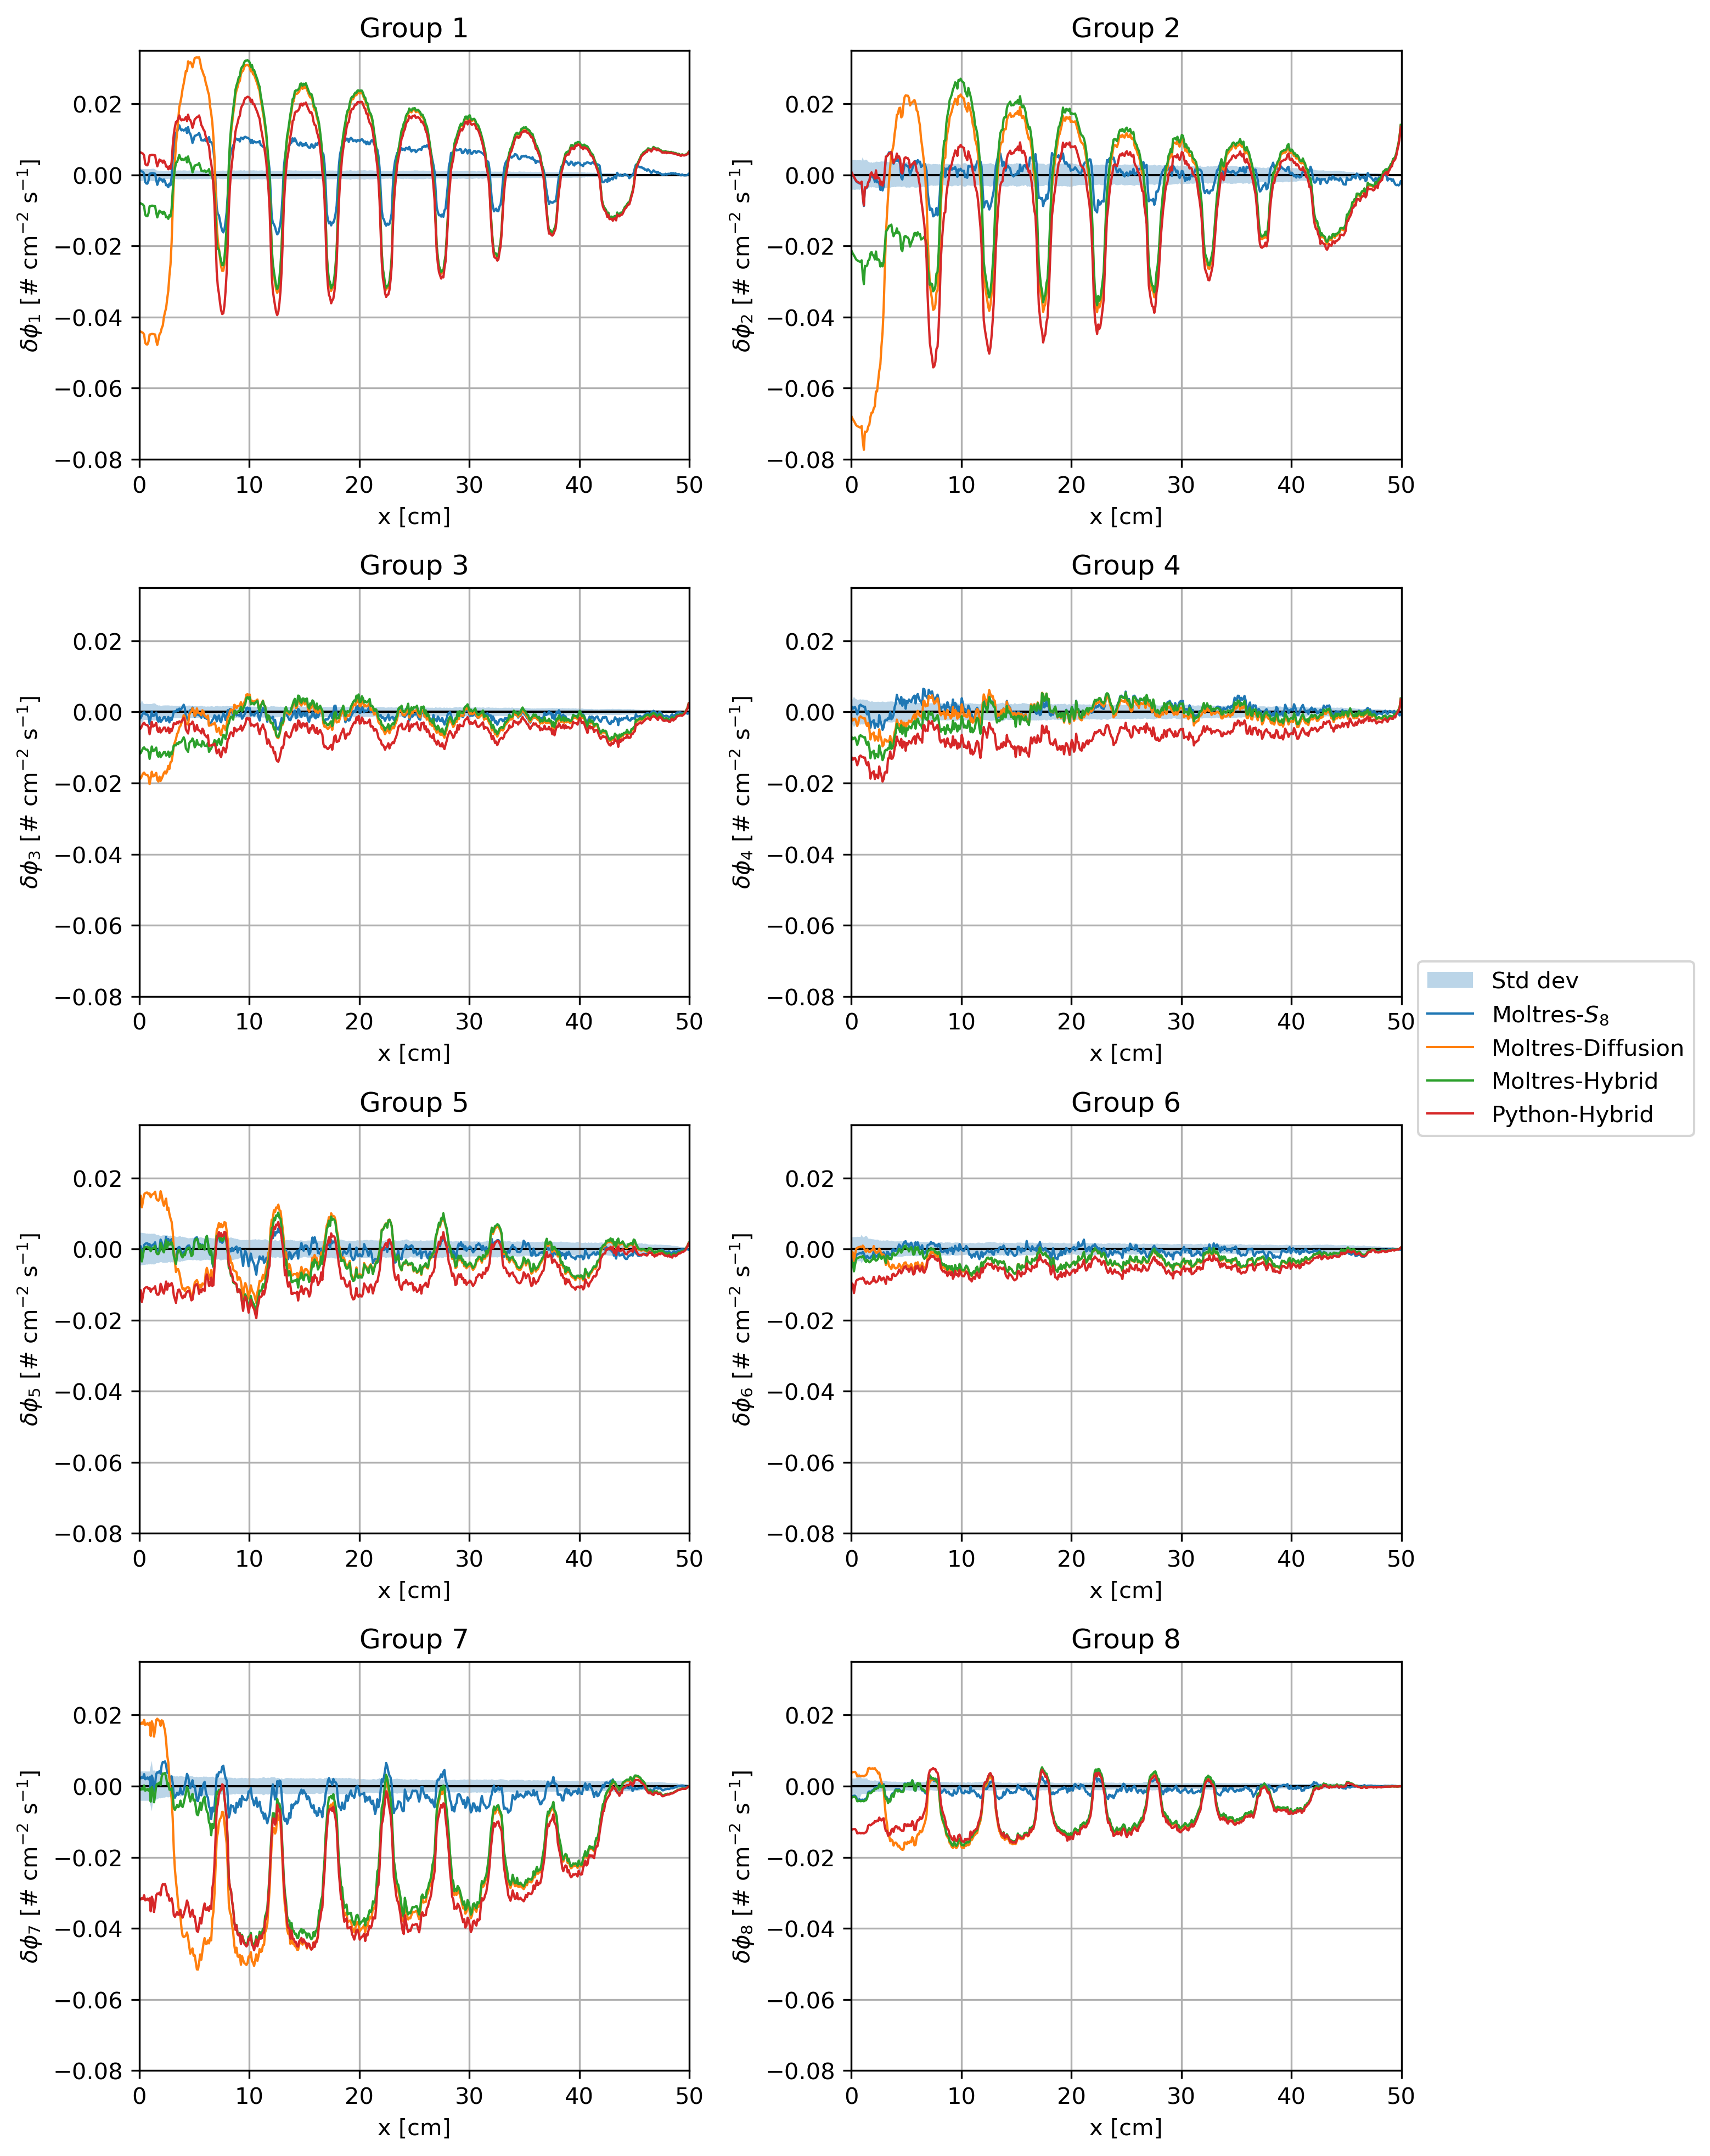
\includegraphics[width=\columnwidth]{case-3a-flux-diff}
  \caption{Absolute difference in neutron group flux distributions for Case 3a from Moltres-$S_8$,
  Moltres-diffusion, Moltres-hybrid, and Python-hybrid relative to OpenMC-MG.}
  \label{fig:3a-flux-diff}
\end{figure}

\begin{figure}[p]
  \centering
  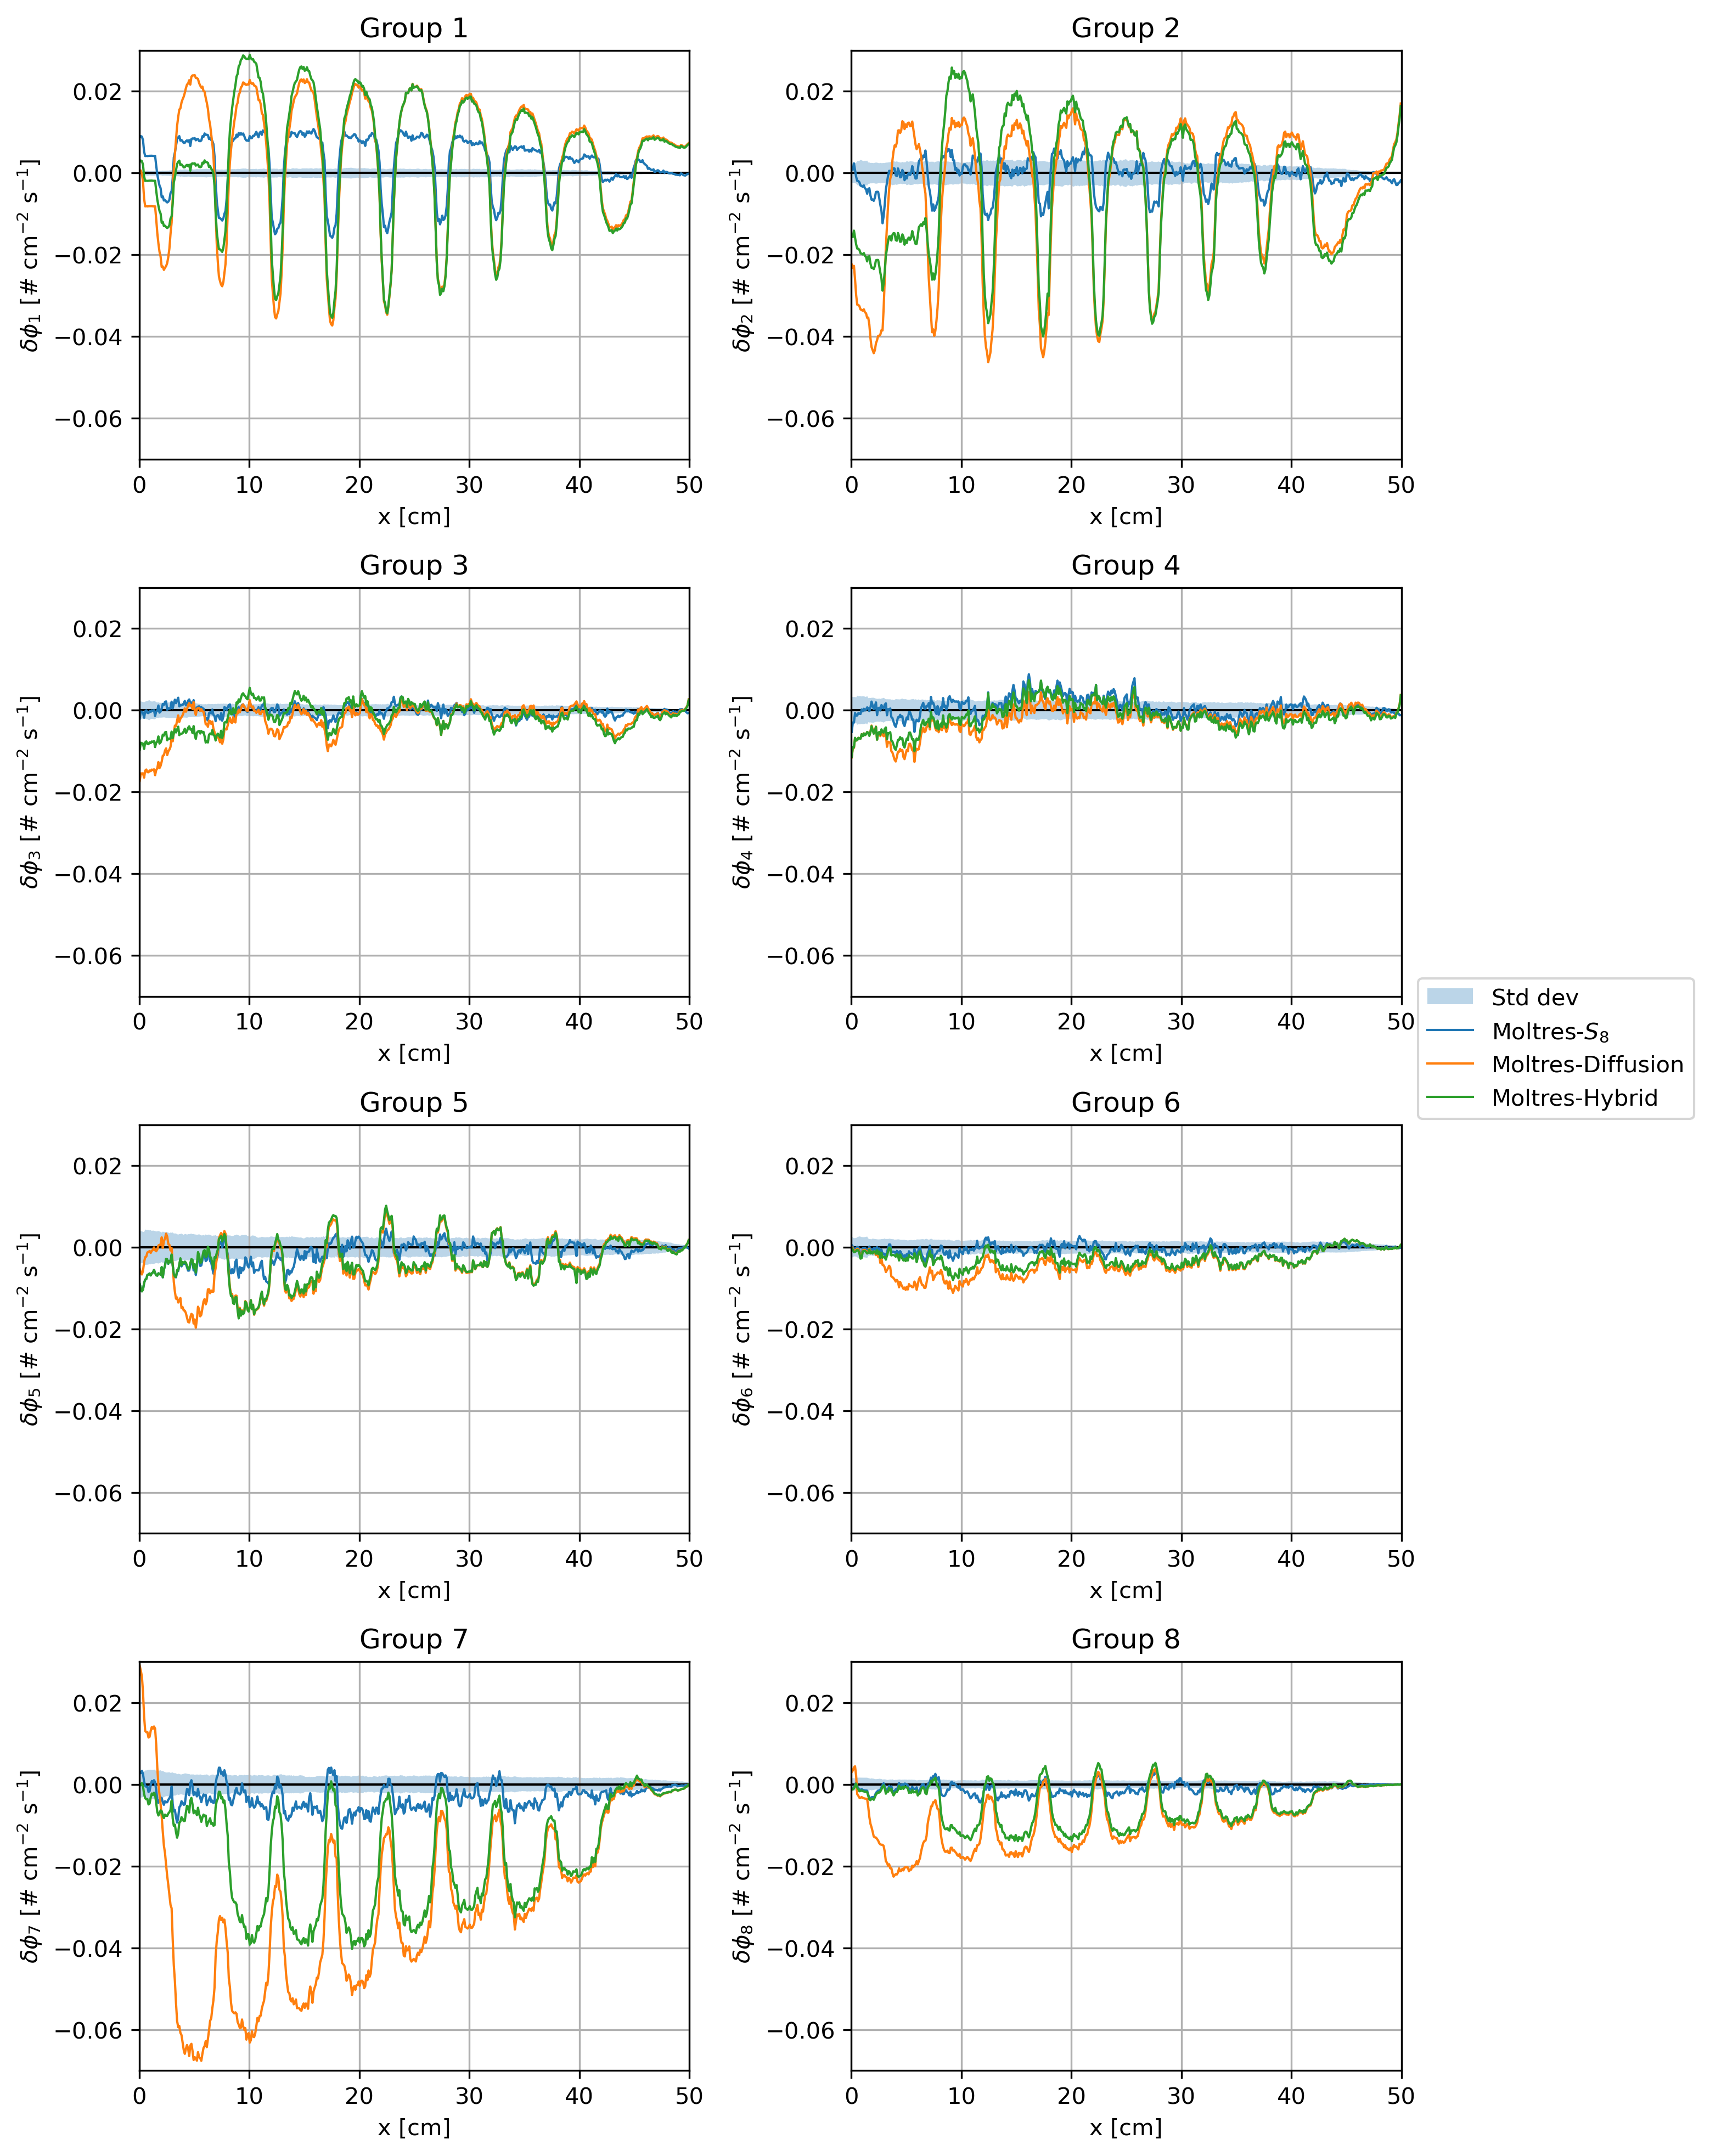
\includegraphics[width=\columnwidth]{case-3b-flux-diff}
  \caption{Absolute difference in neutron group flux distributions for Case 3b from Moltres-$S_8$,
  Moltres-diffusion, Moltres-hybrid, and Python-hybrid relative to OpenMC-MG.}
  \label{fig:3b-flux-diff}
\end{figure}

\FloatBarrier

%\subsubsubsection{Drift \& diffusion correction distribution}

Figure \ref{fig:3b-drift} shows the distributions of the drift correction parameter in each neutron
energy group for Case 3b. The hybrid method selectively applies the $S_N$ method to improve
neutronic modeling within the subregions. We computed
the reference distributions (orange data points) in both plots from reference flux solutions of the
standard $S_8$ method.
As discussed in Section \ref{sec:buffer-region}, the drift correction parameter matches the
reference values within the correction subregion
from $x=0$ cm to 10 cm except near the subregion boundary at $x=10$ cm.
%Therefore, both schemes
%provide improved flux estimates in the subregion compared to the neutron diffusion method.

In Figure \ref{fig:3b-drift}, the drift
correction distributions for all eight energy groups are well-defined throughout
the subregion and are continuous except at material interfaces. Consequently, the drift correction
scheme provides accurate flux corrections for about 75\% of the subregion based on the buffer
region cutoff criteria which occurs around $x=7.5$ cm where most of the drift distributions are
zero (refer to Section \ref{sec:buffer-region}).

\begin{figure}[p]
  \centering
  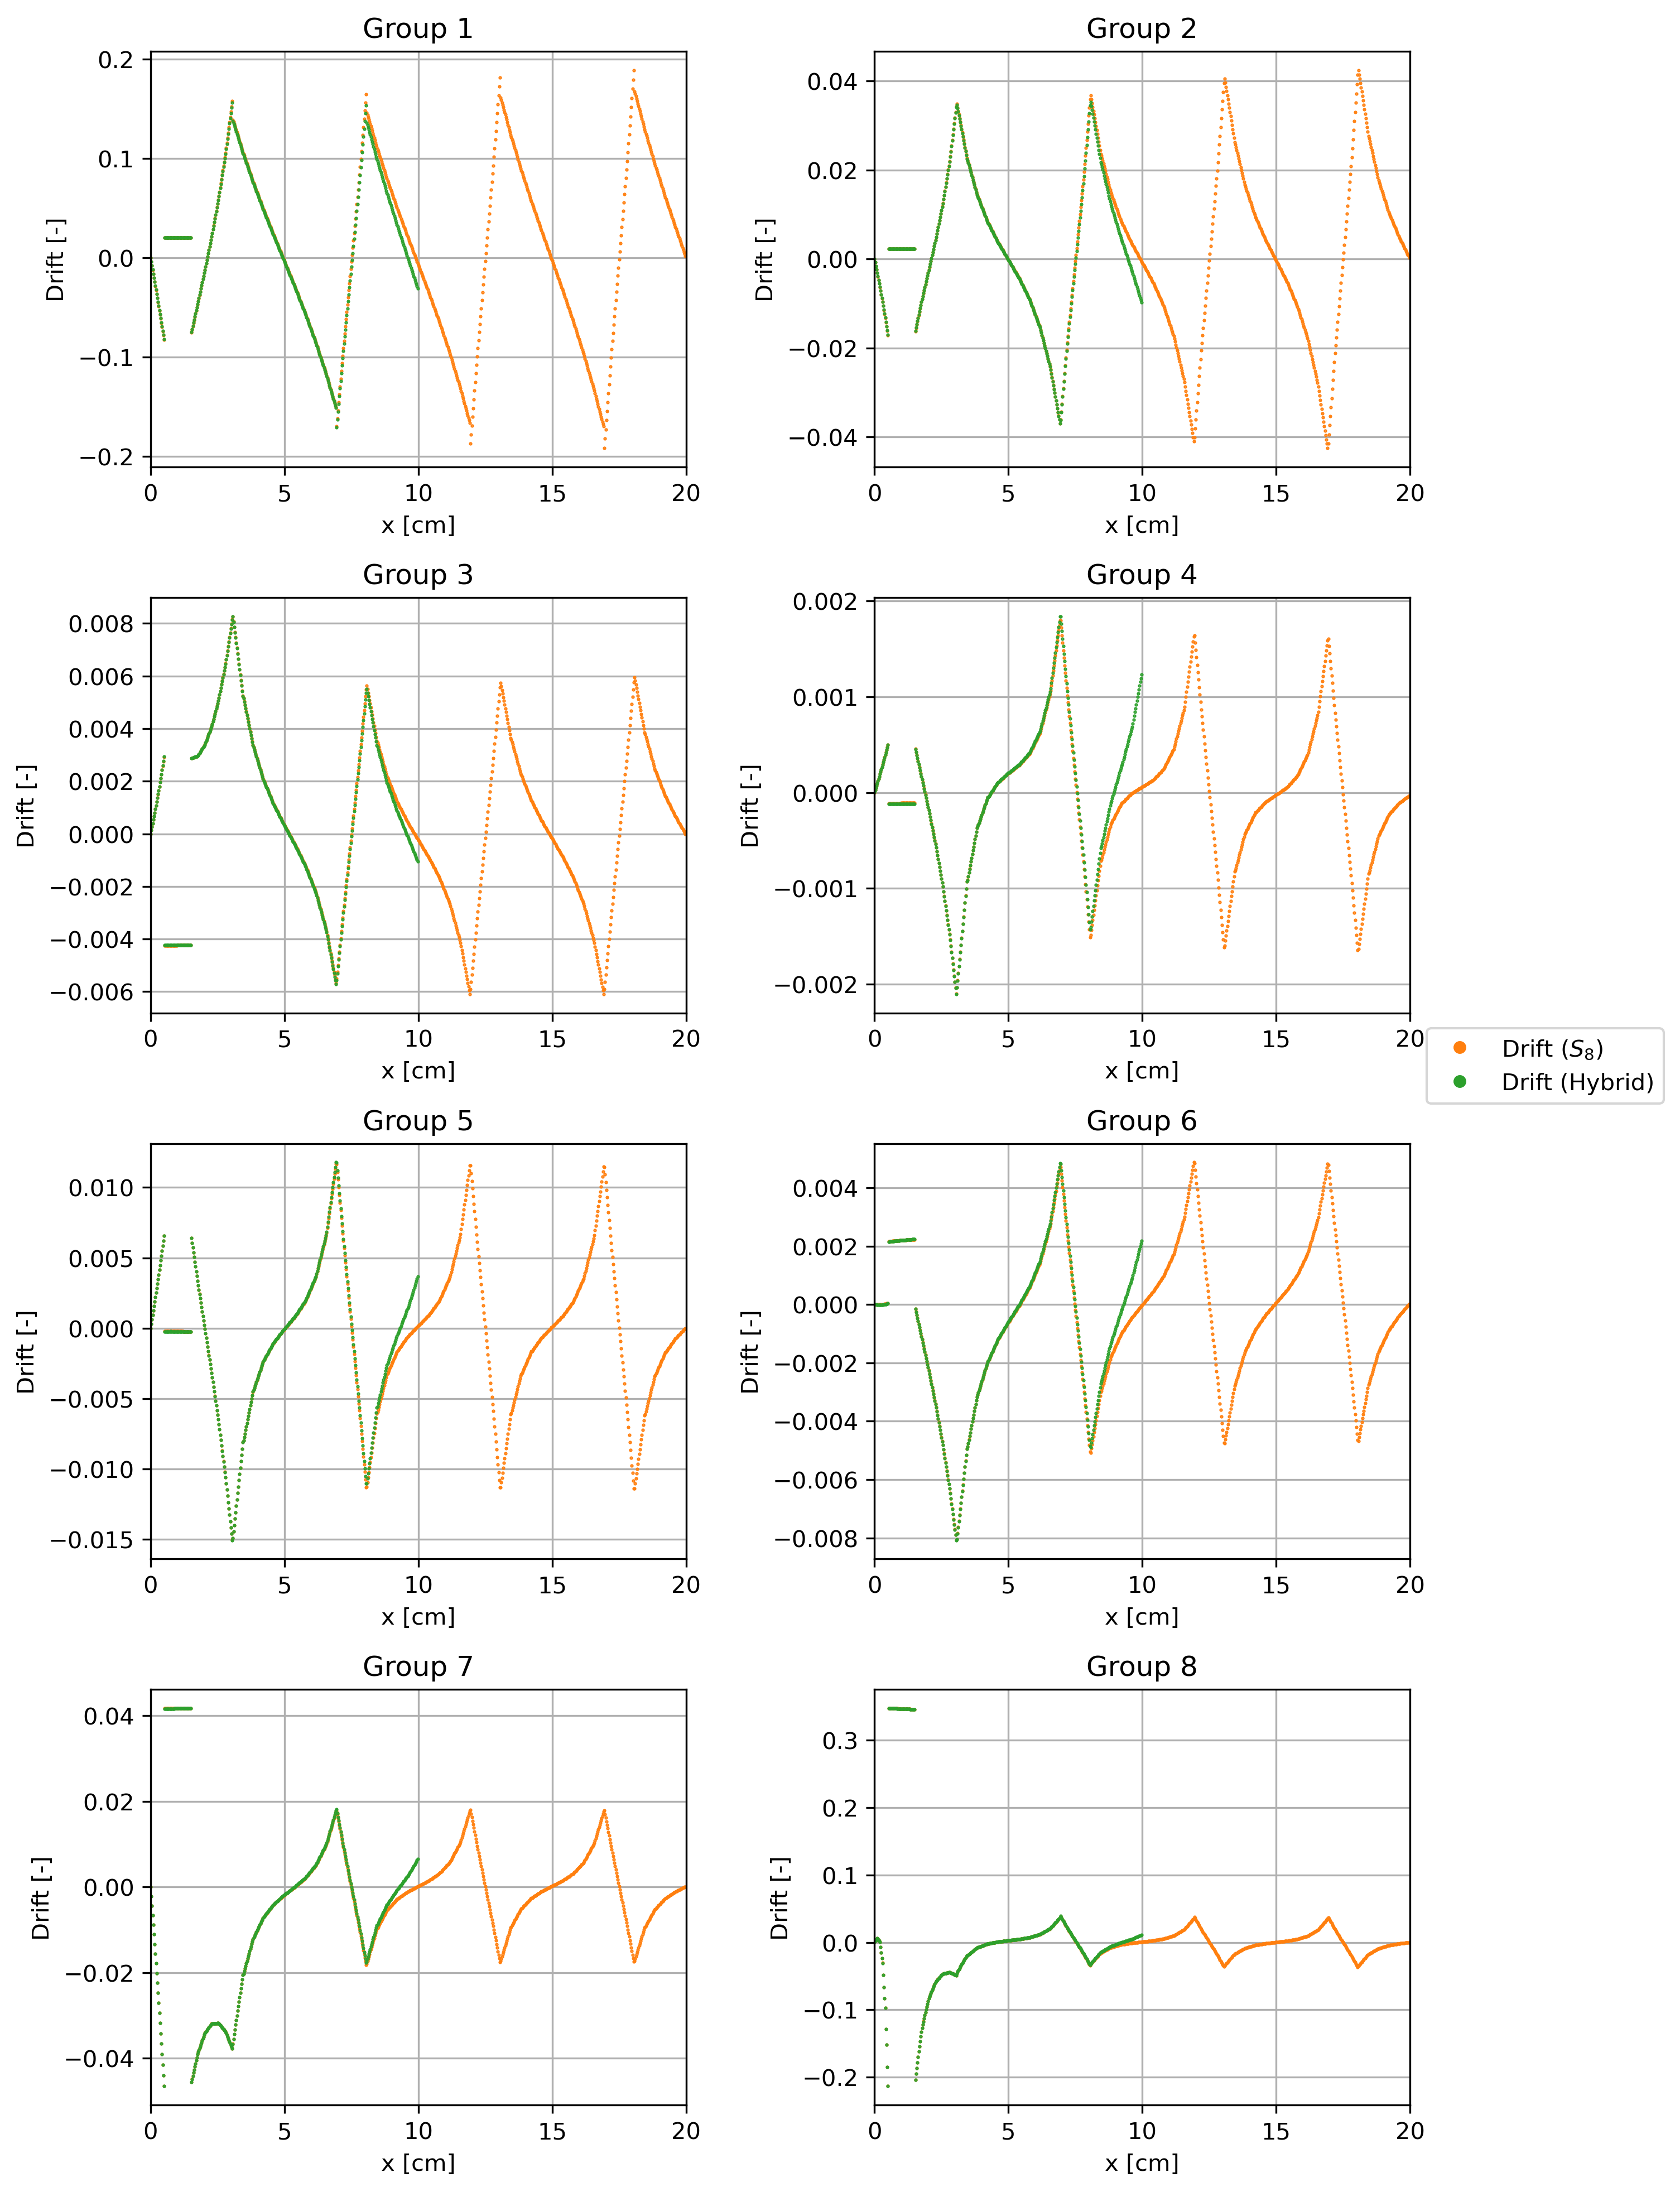
\includegraphics[width=.99\columnwidth]{case-3b-drift}
  \caption{Multigroup drift correction ($\vec{D}_g$) $x$-component distributions from the
  Moltres-hybrid and Moltres-$S_8$ solvers.}
  \label{fig:3b-drift}
\end{figure}

%\begin{figure}[thb]
%  \centering
%  \includegraphics[width=.99\columnwidth]{case-3b-svdc}
%  \caption{Multigroup diffusion correction ($D^s_g$) $x$-component distributions from the
%    Python-hybrid and Python-$S_8$ solvers.}
%  \label{fig:3b-svdc}
%\end{figure}

\FloatBarrier

%\subsubsubsection{Impact of correction subregion sizes}

The hybrid $S_N$-diffusion method relies on $S_N$ calculations in the correction subregion to
generate flux corrections. Minimizing the size of the correction subregion and the $S_N$ subproblem
is essential for the hybrid method to be computationally competitive for time-dependent full-core
simulations. We investigated the effect of the correction subregion size on the $k_\text{eff}$ and
control rod worth estimates with Cases 3a and 3b by varying the subregion sizes from 10 cm to 40 cm
at 5 cm-intervals. All subregion sizes place the subregion boundary more than 1 neutron mean free
path away from the control rod. The shortest measured neutron mean free paths are 4.81 cm and 5.85
cm for group 1 neutrons in the fuel and graphite regions, respectively.

Figures \ref{fig:v1-size-a-k} and \ref{fig:v1-size-b-k} show the $k_\text{eff}$ estimates from the
hybrid method for Cases 3a and 3b, respectively. In both cases, the $k_\text{eff}$ values initially
decrease as the correction subregion sizes increase before reversing in trend when the subregion
size reaches 35 cm and beyond. The $k_\text{eff}$ values vary by up to 164 pcm for Case 3a and 109
pcm for Case 3b. An important observation here is that the $k_\text{eff}$ values do not
monotonically converge towards the $k_\text{eff}$ estimate from the $S_8$ method. This behavior
implies that neutron leakage error at the outer boundary remains a significant source of
discrepancy as long as the correction region does not encompass the outer boundary.

\begin{figure}[htb!]
  \centering
  \begin{subfigure}[b]{0.49\columnwidth}
    \centering
    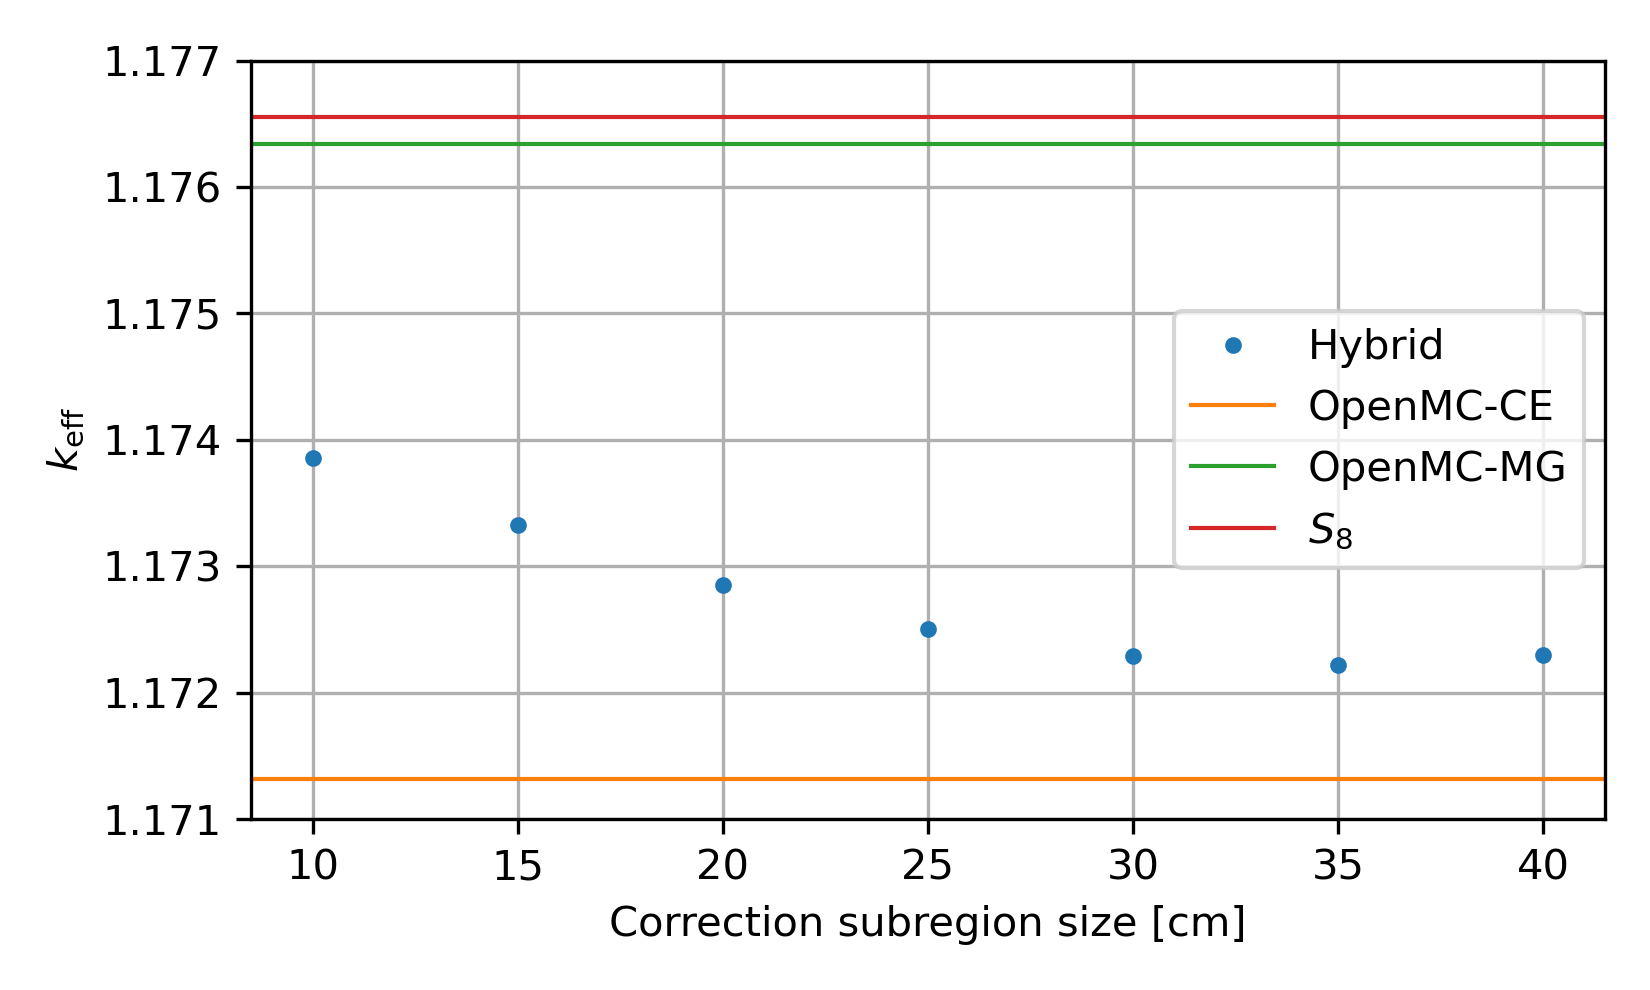
\includegraphics[width=\columnwidth]{correction-size-a-k}
    \caption{Case 3a}
    \label{fig:v1-size-a-k}
  \end{subfigure}
  \hfill
  \begin{subfigure}[b]{0.49\columnwidth}
    \centering
    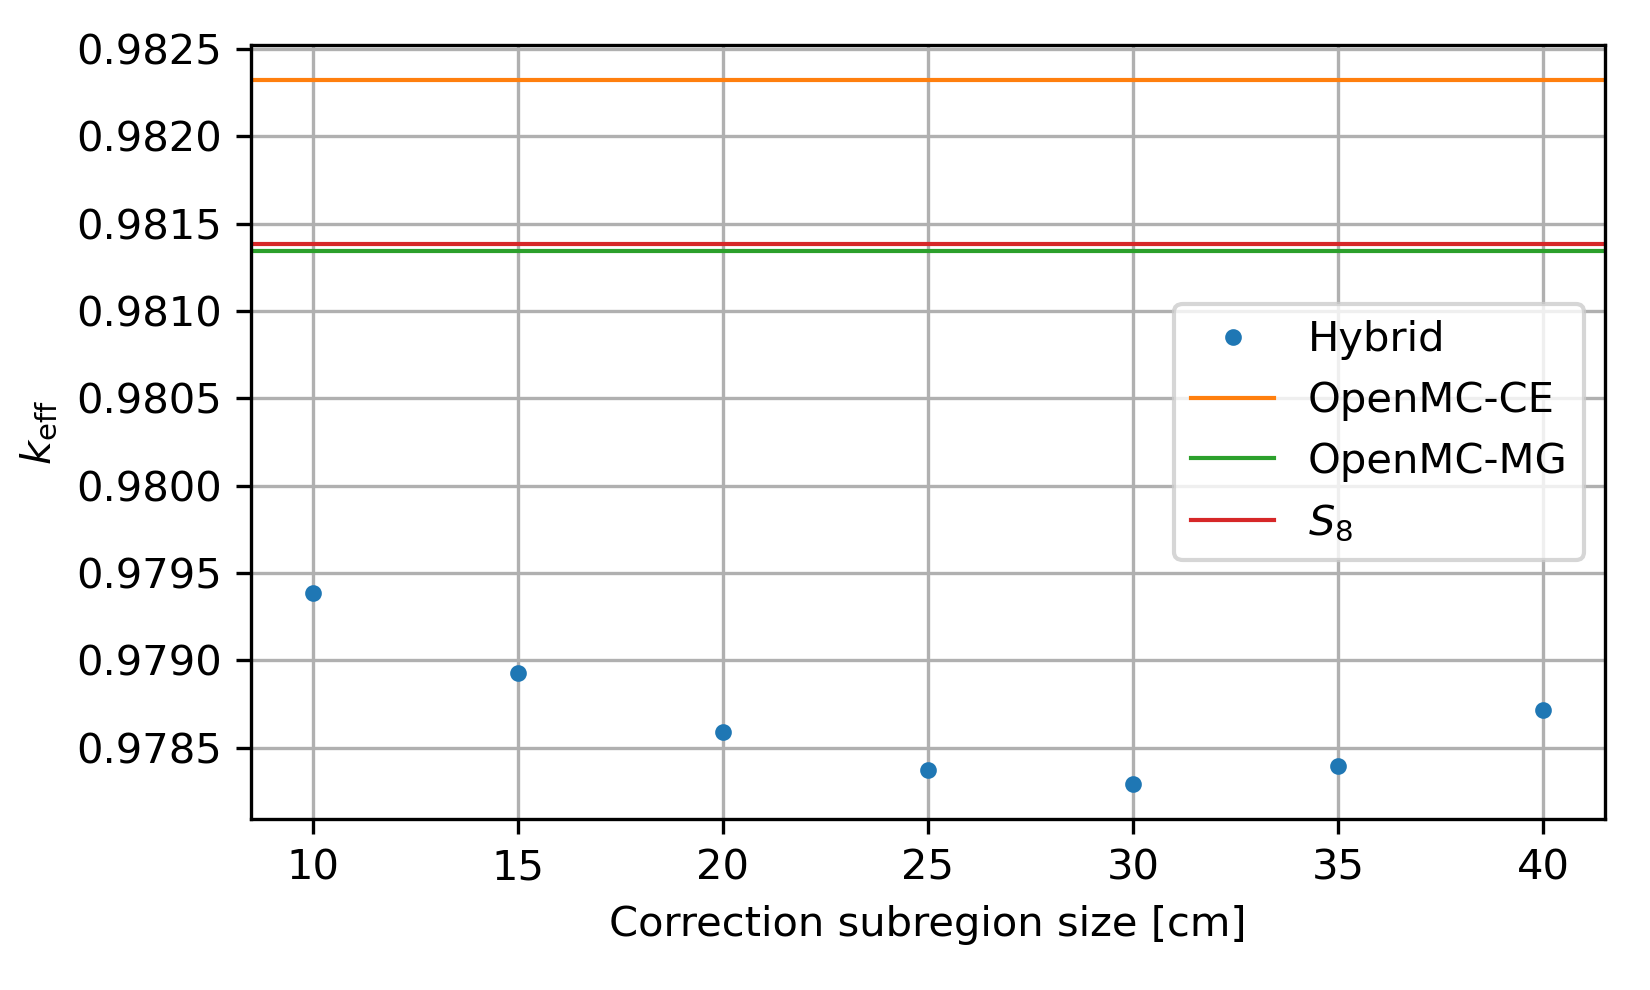
\includegraphics[width=\columnwidth]{correction-size-b-k}
    \caption{Case 3b}
    \label{fig:v1-size-b-k}
  \end{subfigure}
  \caption{$k_\text{eff}$ estimates from the hybrid method for Cases 3a and 3b with different
  correction subregion sizes. The horizontal lines indicate $k_\text{eff}$ estimates from the
  OpenMC-CE, OpenMC-MG, and $S_8$ methods.}
  \label{fig:v1-size-k}
\end{figure}

Figure \ref{fig:v1-size-rho} shows the percentage difference in rod worth relative to OpenMC-CE. 
Due to the identical trends observed in the $k_\text{eff}$ estimates of both cases, the control rod
worth estimates do not change significantly when the correction subregion
sizes change. The rod worth estimates for all investigated correction subregion sizes remain within
0.2\% of the $S_8$ method. This indicates limiting the correction subregion size to save
computational cost on the expensive $S_N$ calculations has a negligible impact on rod worth
estimates.

\begin{figure}[htb!]
  \centering
  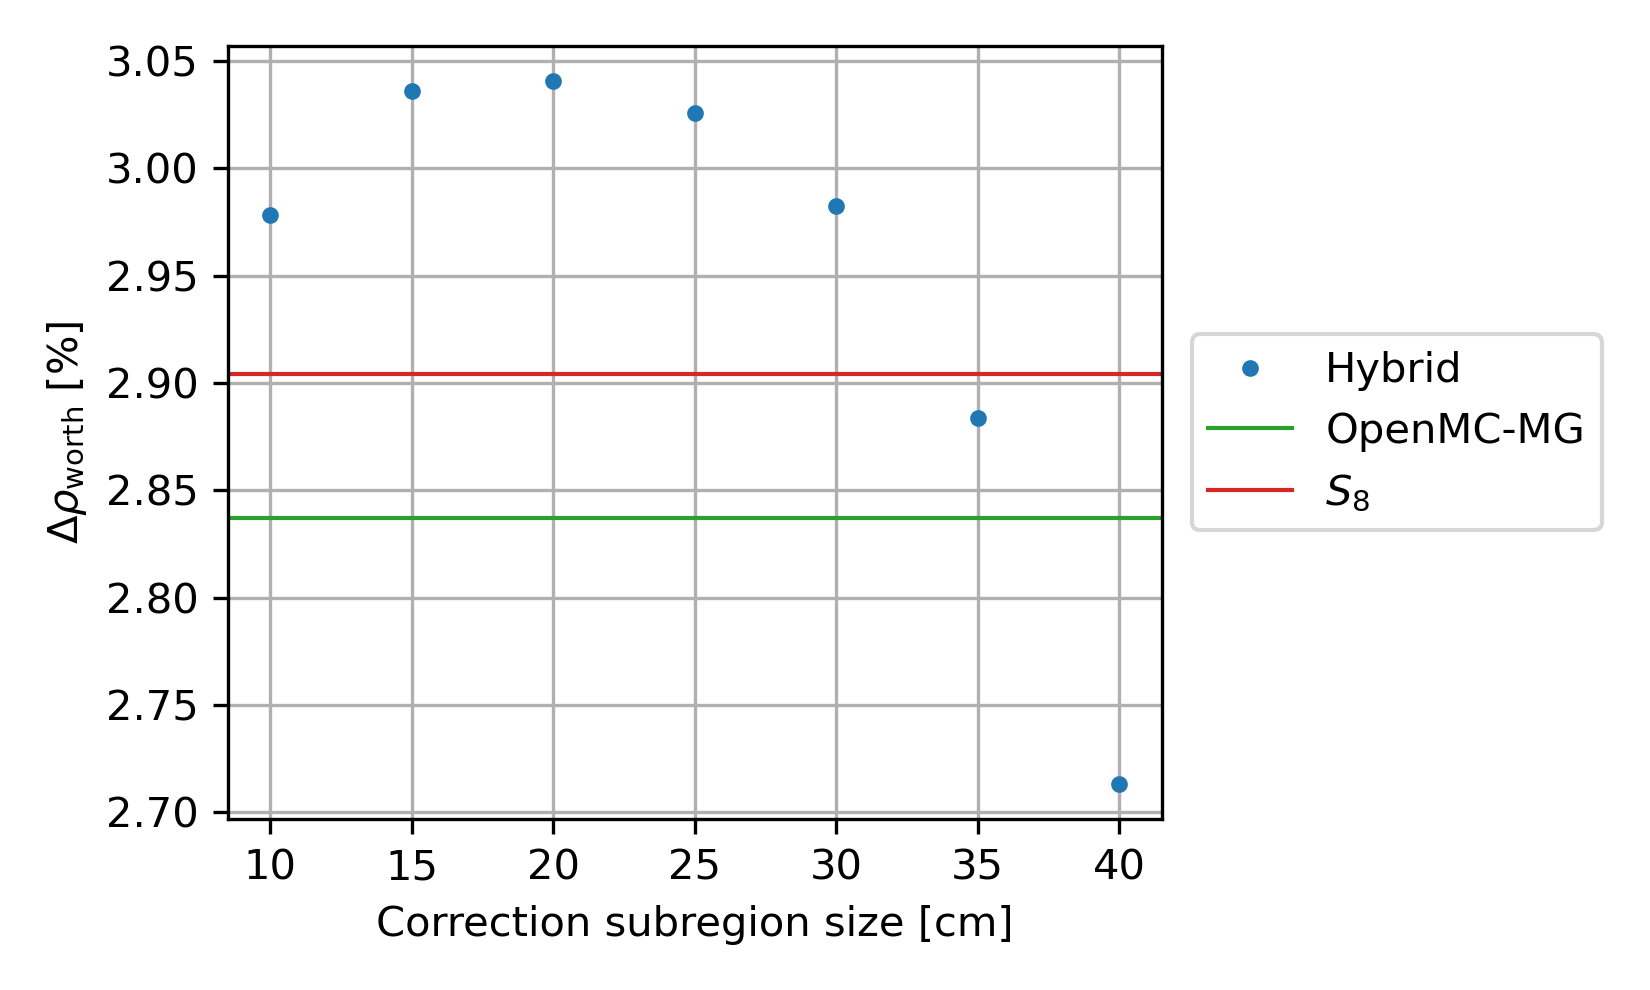
\includegraphics[width=0.8\columnwidth]{correction-size-rho}
  \caption{Percentage difference in rod worth from the hybrid method relative to OpenMC-CE for
    Cases 3a and 3b with different correction subregion sizes. The horizontal lines indicate
    equivalent rod worth differences from the OpenMC-MG and $S_8$ methods.}
  \label{fig:v1-size-rho}
\end{figure}

The $k_\text{eff}$ and rod worth results show the hybrid method is able to accurately
reproduce rod worth estimates as long as the correction subregion size remains consistent between
$k$-eigenvalue simulations used for rod worth calculations. The
correction subregion size must also be sufficiently large to capture the highly neutron-absorptive
rod's influence on the neutron flux around the rod at $x=0$ cm. The drift correction parameter
distributions in Figure \ref{fig:3b-drift} indicate that the influence of the rod on the drift, and
consequently the flux, extend to approximately $x=5$ cm before the drift distribution settles on a
regular repeating pattern influenced by the fuel-graphite lattice structure. The Case 2 and 3
simulations applied a consistent
correction subregion size of 10 cm since this size sufficiently meets the requirements
discussed while also minimizing the computational cost of the $S_8$ subsolver. Other reactor
designs consisting of different material components may require different minimum correction
subregion sizes.

%\subsubsubsection{Relaxing the $S_N$ subsolver convergence threshold}

As described in Sections \ref{sec:hybrid-algorithm} \& \ref{sec:numerical-implementation}, the
hybrid $S_N$-diffusion method works by iteratively coupling a neutron diffusion solver and a $S_N$
subsolver with the latter generating drift correction parameters for the former.
The hybrid method shares some similarities with diffusion-based \gls{HOLO} acceleration schemes
for the neutron transport methods which do not
require the neutron transport side of the calculations to fully converge
\cite{reynolds_analysis_2023, wang_diffusion_2014}. The typical convergence threshold value
required for converged neutron flux calculations in Moltres is $10^{-8}$; the convergence tolerance
value was set to $10^{-8}$ for the neutron diffusion solver and the fixed point scheme. We
investigated a range of convergence tolerance values for the $S_N$ subsolver to 
find the optimal value for maintaining sufficient solution accuracy and minimizing computational
costs; tightening the $S_N$ convergence tolerance value generally results in more outer iterations
performed before the solver meets the fixed point convergence tolerance.
Table \ref{table:sn-tol} lists the number of outer iterations required by the hybrid method for
a given set of $S_8$ subsolver convergence tolerance values in Case 3b.

\begin{table}[h]
  \centering
  \caption{Number of outer iterations in hybrid method calculations of Case 3b for a given set of
  convergence tolerance values imposed on the $S_8$ subsolver.}
  \begin{tabular}{l S S S S S S}
    \toprule
    $S_8$ subsolver tolerance, $\epsilon_\text{tol}$ & {$10^{-8}$} & {$10^{-7}$} & {$10^{-6}$} & {$10^{-5}$} & {$10^{-4}$} & {$10^{-3}$} \\
    \midrule
    Number of outer iterations & 3 & 3 & 3 & 2 & 2 & 1 \\
    \bottomrule
  \end{tabular}
  \label{table:sn-tol}
\end{table}
%
\begin{figure}[h]
  \centering
  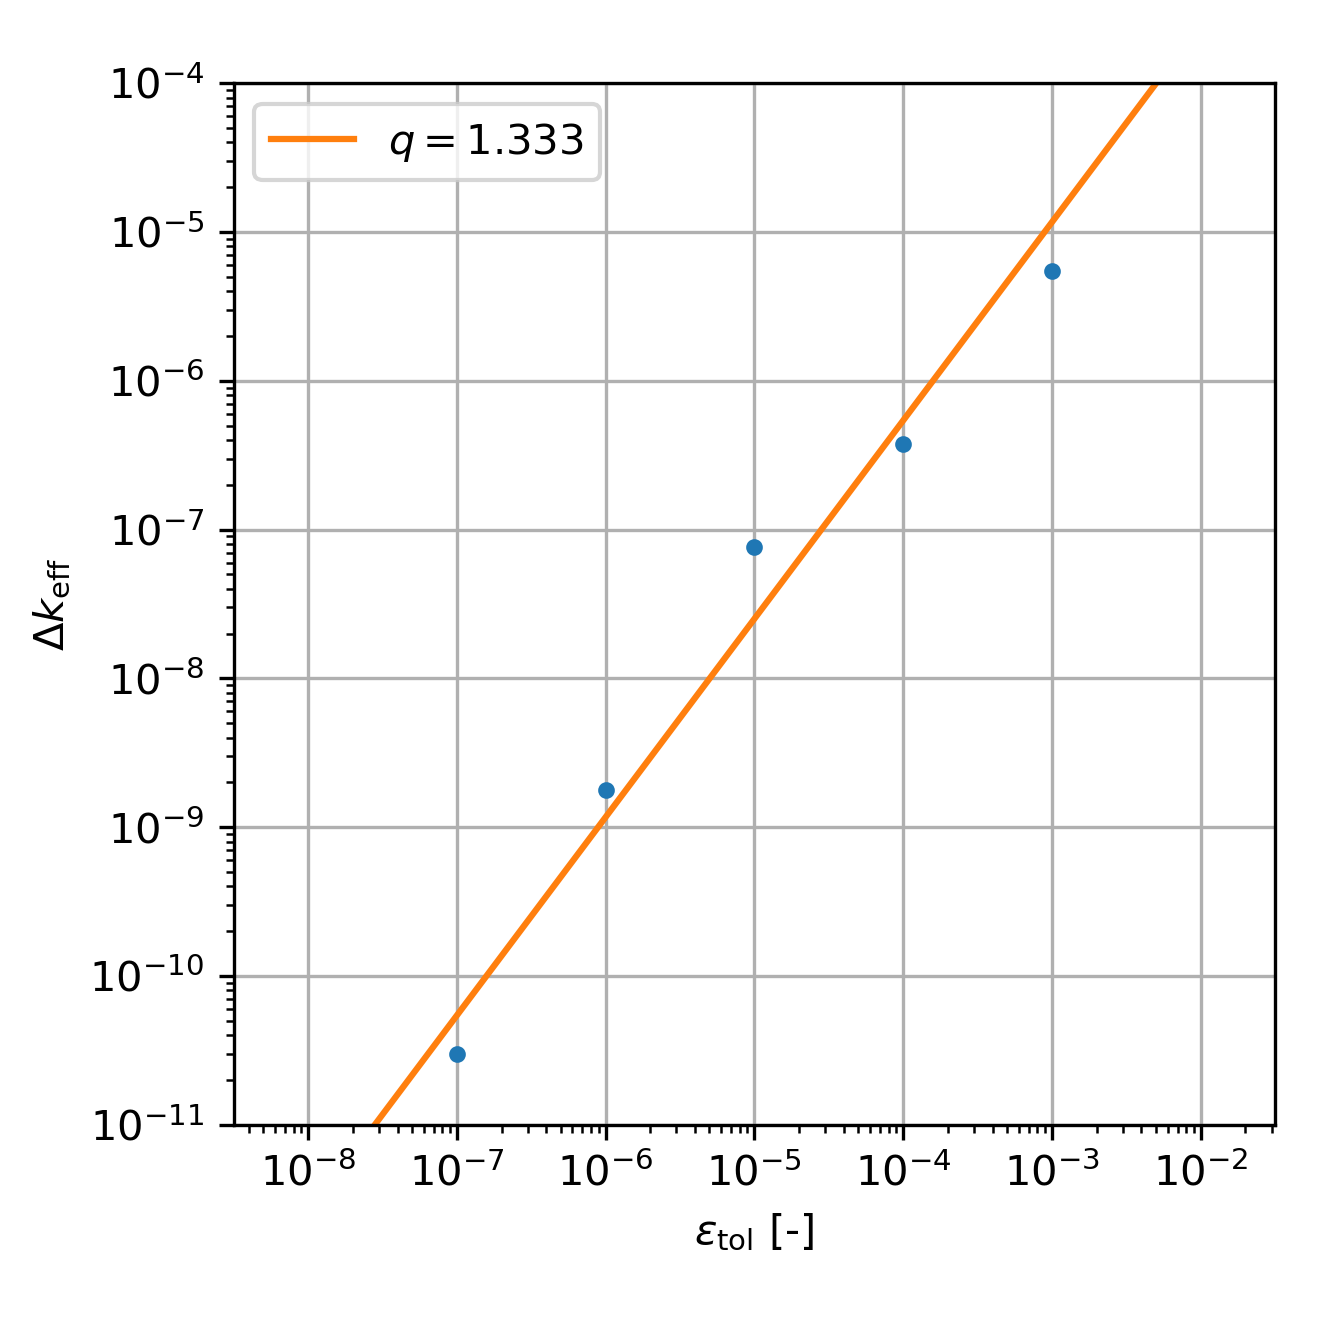
\includegraphics[width=0.6\columnwidth]{sn-tol}
  \caption{$k_\text{eff}$ error estimates of Case 3b for a range of convergence tolerance values
  imposed on the $S_8$ subsolver relative to the reference $k_\text{eff}$ value when
  $\epsilon_\text{tol}=10^{-8}$. The $q=1.333$ line represents the approximate rate of
  convergence.}
  \label{fig:sn-tol}
\end{figure}

Figure \ref{fig:sn-tol} shows the $k_\text{eff}$ error estimates relative to the reference value
when $\epsilon_\text{tol}=10^{-8}$. The hybrid method exhibits superlinear convergence ($q=1.333$)
with respect to the $S_N$ subsolver convergence tolerance value. Based on the results, setting
$\epsilon_\text{tol}$ to $10^{-5}$ is a good balance between accuracy and computational
cost because the $k_\text{eff}$ error is less than 0.01 pcm and the number of outer iterations
would increase from 2 to 3 if the tolerance value is further tightened.

\FloatBarrier

\subsection{2-D Neutronics Models \& Results} \label{sec:2d-results}

This section presents the models, results, and discussion of the 2-D cases. Section
\ref{sec:2d-model-setup} describes the model setup of the 2-D cases. Section
\ref{sec:2d-nts-results} covers the results and discussion of the 2-D cases.

\subsubsection{2-D Neutronics Model Setup} \label{sec:2d-model-setup}

Figures \ref{fig:1/4-geom} and \ref{fig:full-geom} show the 2-D quarter-core and full-core
\gls{MSRE} models investigated. This work adapted the models from the horizontal cross section of
the \gls{MSRE} numerical benchmark model \cite{fratoni_molten_2020} with the
following differences in the 2-D \gls{MSRE} model for this work:

\begin{itemize}
  \item Neglected thermal expansion of all reactor components.
  \item Modeled the control rods as perfectly annular cylinders instead of beaded control elements
    strung on flexible steel cables. Neglected the inconel shells encasing the control elements and
    the steel helical cables linking the control elements together.
  \item Set channel pitch, width, and length to 2, 0.2, and 1.2 inches, respectively.
  \item Homogenized the INOR-8 (inconel alloy reactor vessel), graphite, and molten salt regions in the sample basket.
  \item Modified the outer edge of the core graphite to be circular with no jagged edges.
  \item Replaced partial channels with full-size channels near the edge of the core graphite.
  \item Ignored the thermal insulation and shield structures outside the core.
\end{itemize}

The differences listed above result in negligible
changes to the $k_\text{eff}$ (refer to Section 5.6) relative to the \gls{MSRE} benchmark model
\cite{fratoni_molten_2020}.

\begin{table}[htb]
  \small
  \centering
  \setlength\tabcolsep{4pt}
  \caption{\gls{MSRE} molten salt composition when the $^{235}$U loading was at 65.25 kg.}
  \begin{tabular}{l S S S S S S S}
    \toprule
    Element & {Li} & {Be} & {Zr} & {Hf} & {$^{234}$U} & {$^{235}$U} & {$^{236}$U} \\
    \midrule
    Composition [kg] & 507.27 & 293.96 & 513.97 & 0.0029 & 0.67 & 65.25 & 0.27 \\
    \bottomrule
  \end{tabular}
  \begin{tabular}{l S S S S S S}
    \toprule
    Element & {$^{238}$U} & {Fe} & {Cr} & {Ni} & {O} & {F} \\
    \midrule
    Composition [kg] & 141.91 & 0.75 & 0.13 & 0.14 & 2.27 & 3103.22 \\
    \bottomrule
  \end{tabular}
  \label{table:2d-salt-composition}
\end{table}

INOR-8, also referred to as Hastelloy N, is a nickel-based alloy used for structural components in
the \gls{MSRE} \cite{robertson_msre_1965}.
Table \ref{table:2d-salt-composition} lists the molten salt composition for the 2-D models. The
$^{235}$U loading of 65.25 kg is the amount at which the \gls{MSRE} first achieved criticality. The
control rods consist of the original \gls{MSRE} 70 wt\% Gd$_2$O$_3$-30 wt\% Al$_2$O$_3$ mixture.
The models impose neutron vacuum boundary conditions on the outermost boundary of the INOR-8
vessel structure. The quarter-core model imposes neutron reflecting boundary conditions along the
left and bottom straight edges (Figure \ref{fig:1/4-geom}). Note that the quarter-core and
full-core models are not identical because the full-core model contains a sample basket instead of
a control rod in the lower-right segment of Figure \ref{fig:full-geom-closeup}.

All cases for the quarter- and full-core models ran on OpenMC under both continuous
energy (OpenMC-CE) and multigroup (OpenMC-MG) modes, and on Moltres with the hybrid $S_N$-diffusion
and neutron diffusion methods. The hybrid method ran with the $S_8$ angular discretization scheme
and up to 2nd-order scattering approximations for the $S_N$ subsolver. The quarter-core model cases
ran with and without the control rod in the air-filled rod thimble; air replaces the
control rod material when the rod is removed. For full-core model, this work considered four rod
configurations: no rods present, rod 1 present, rods 1 \& 2 present, and rods 1, 2 \& present.
Other than providing a close-up view of the core center, Figure \ref{fig:full-geom-closeup} also
presents the correction subregion on which the $S_8$ subsolver of the hybrid method generates
drift correction parameters for the coupled diffusion solver.

\begin{figure}[p]
  \centering
  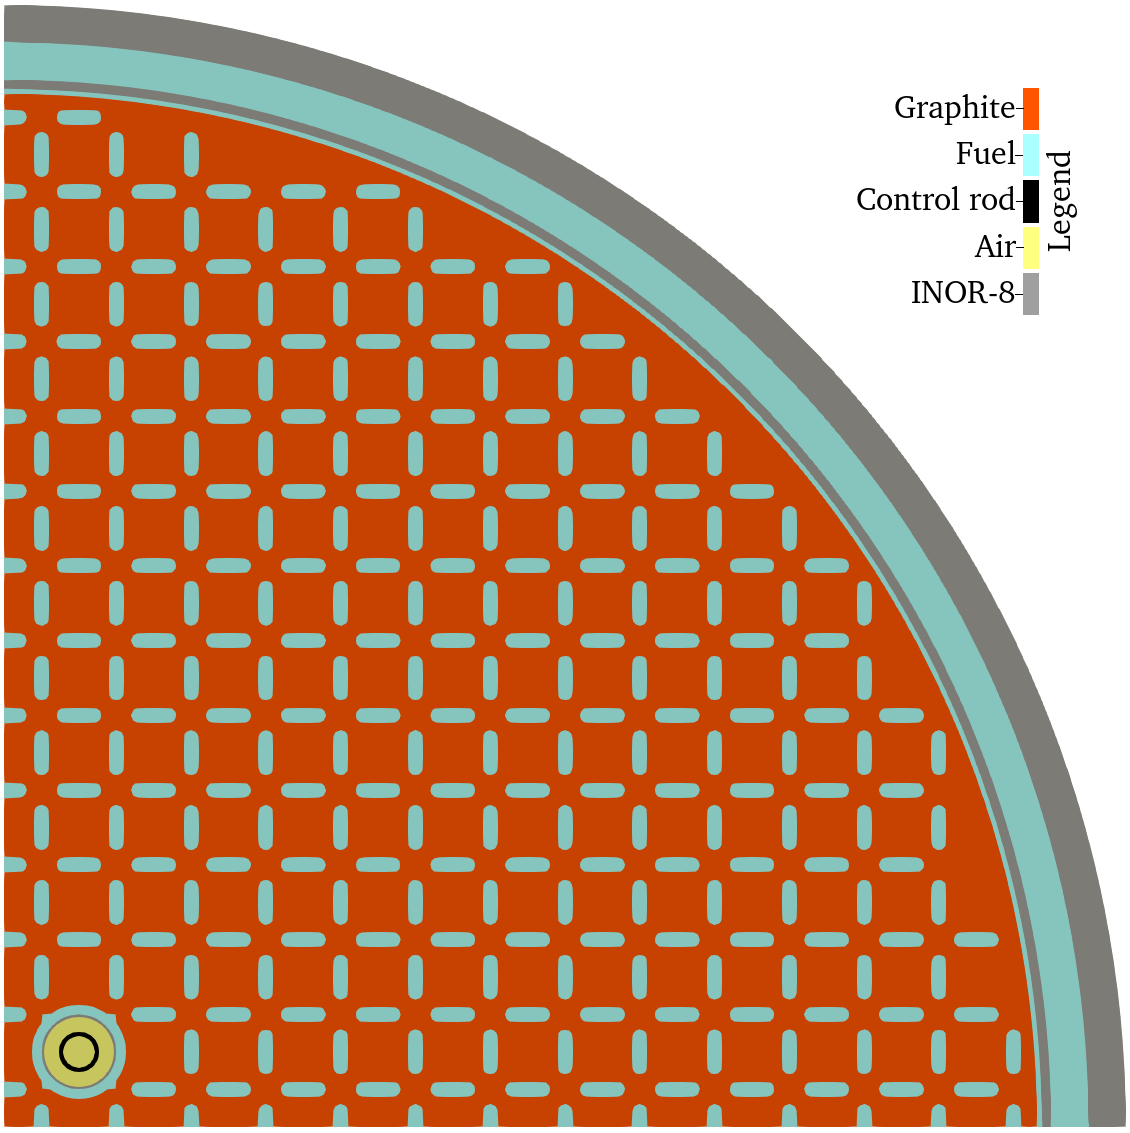
\includegraphics[width=\columnwidth]{quarter-core-geom}
  \caption{2-D \gls{MSRE} quarter-core model based on the horizontal cross section of the actual
  \gls{MSRE} geometry.}
  \label{fig:1/4-geom}
\end{figure}

\begin{figure}[p]
  \centering
  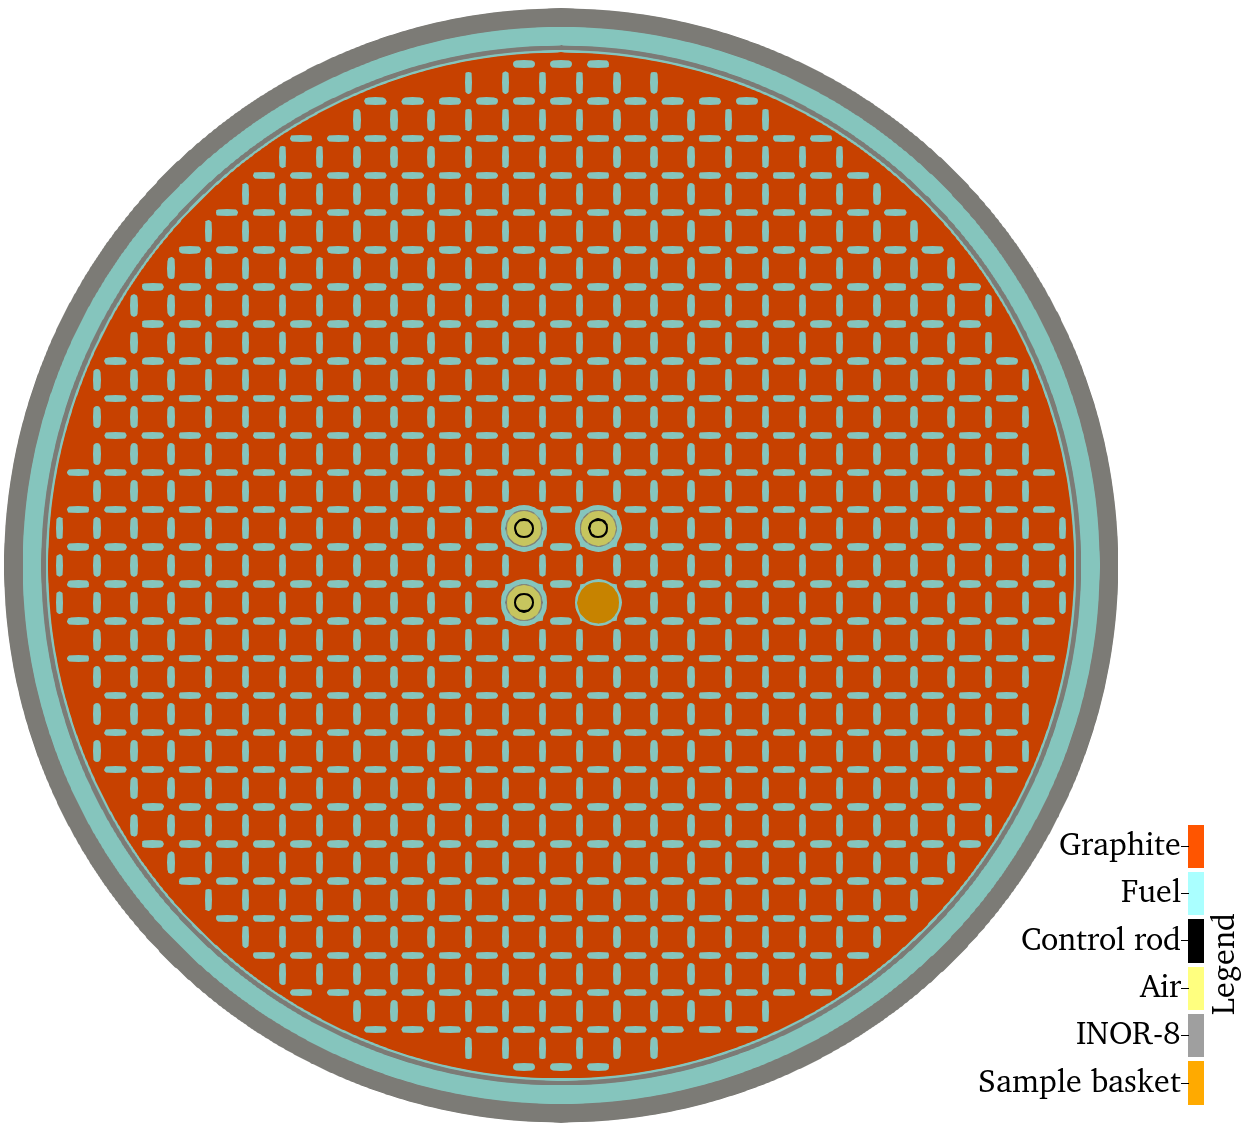
\includegraphics[width=\columnwidth]{full-core-geom}
  \caption{2-D \gls{MSRE} full-core model based on the horizontal cross section of the actual
  \gls{MSRE} geometry.}
  \label{fig:full-geom}
\end{figure}

\begin{figure}[p]
  \centering
  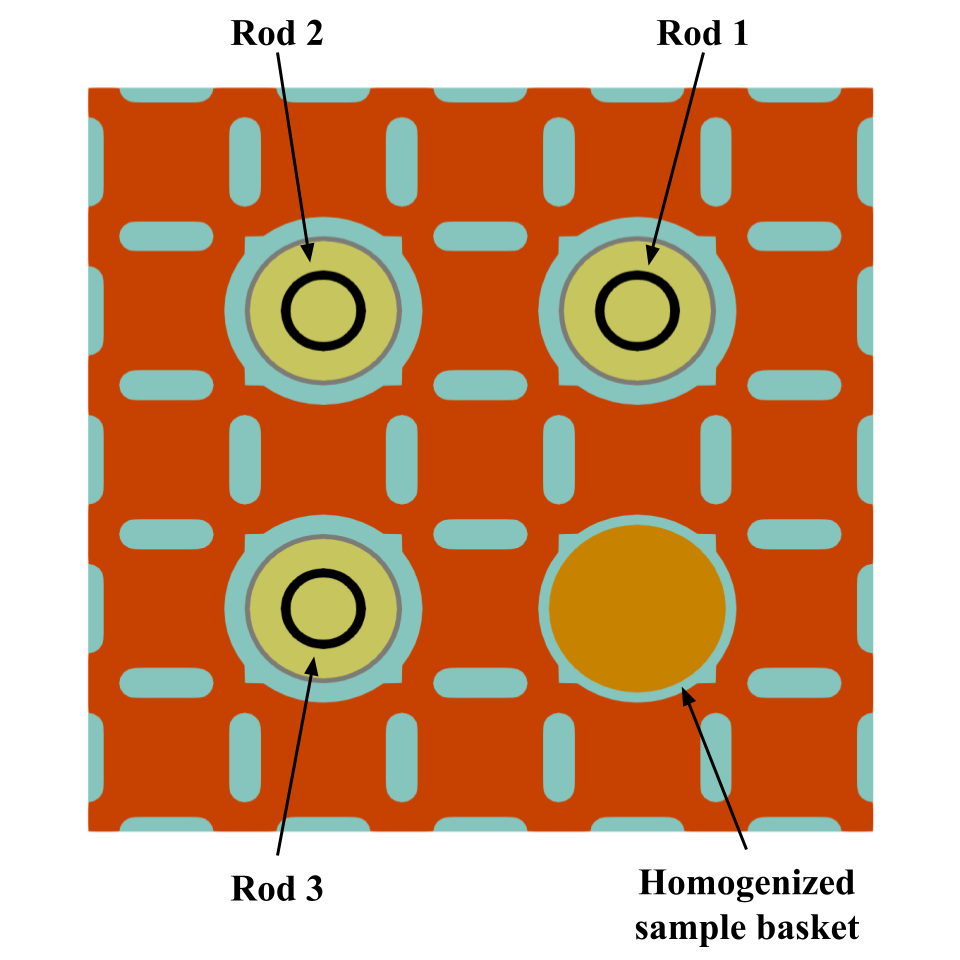
\includegraphics[width=0.7\columnwidth]{full-core-closeup}
  \caption{Detailed view of the control rod thimbles and sample basket in 2-D \gls{MSRE} full-core
    model.}
  \label{fig:full-geom-closeup}
\end{figure}

%\FloatBarrier

\subsubsection{2-D Numerical Results \& Discussion} \label{sec:2d-nts-results}

This subsection presents the results and discussion of the 2-D quarter-core and full-core models.

%\subsubsubsection{2-D Quarter-Core}

Table \ref{table:quarter-core} details the $k_\text{eff}$ and control rod worth estimates and error
values relative to OpenMC-CE. For the ``No Rod'' case, OpenMC-CE estimated the $k_\text{eff}$ to be
1.11209(43). The OpenMC-MG, hybrid, and neutron diffusion methods performed
similarly to one another with reactivity errors ranging from 618 pcm to 773 pcm relative to
OpenMC-CE. Based on $k_\text{eff}$ alone, the hybrid method performed marginally worse than the
neutron diffusion method. However, for the ``Rod'' case, then neutron diffusion method saw a
change in sign of the error to -816 pcm. The errors for OpenMC-MG and the hybrid method
remained positive and reduced to 446 pcm and 760 pcm, respectively. Consequently, when taking the
difference in reactivities to estimate the rod worth, the neutron diffusion method performed
significantly worse than OpenMC-MG and the hybrid method. OpenMC-CE estimated the rod worth to be
8370(53) pcm. The neutron diffusion method overestimated the rod worth by 1484 pcm. The hybrid
method improved significantly over the neutron diffusion method with a rod worth estimate that is
only 13 pcm higher than OpenMC-CE. OpenMC-MG reported a larger error of 172 pcm. This is likely due
to statistical uncertainty in OpenMC-MG and favorable error cancellation between different sources
of error in the hybrid method (e.g., neutron leakage, heterogeneous core geometry).
The OpenMC-CE and OpenMC-MG rod worth estimates agree within two standard deviations of each other.

\begin{table}[htb]
  \small
  \centering
  \caption{$k_\text{eff}$ and control rod worth estimates for the 2-D quarter-core \gls{MSRE}
    model. Error values are relative to OpenMC-CE.}
  \begin{tabular}{l S[table-format=1.5(2)] S S[table-format=1.5(2)] S S[table-format=4(2)] S}
    \toprule
    \multirow{2}{*}{Method} & \multicolumn{2}{c}{No Rod} & \multicolumn{2}{c}{Rod} & \multicolumn{2}{c}{Rod worth} \\
                            & {$k_\text{eff}$} & {Error [pcm]} & {$k_\text{eff}$} & {Error [pcm]} & {$\Delta\rho_\text{worth}$ [pcm]} & {Error [pcm]} \\
                            \cmidrule(r){1-1} \cmidrule(rl){2-3} \cmidrule(rl){4-5} \cmidrule(l){6-7}
	  OpenMC-CE & 1.11209(43) & {-} & 1.01740(42) & {-} & 8370(53) & {-} \\
	  OpenMC-MG & 1.11979(42) & 618 & 1.02204(41) & 446 & 8541(51) & 172 \\
      Diffusion & 1.12059 & 682 & 1.00903 & -816 & 9867 & 1484 \\
      Hybrid & 1.12174 & 773 & 1.02532 & 760 & 8383 & 13 \\
    \bottomrule
  \end{tabular}
  \label{table:quarter-core}
\end{table}

\begin{figure}[p]
  \centering
  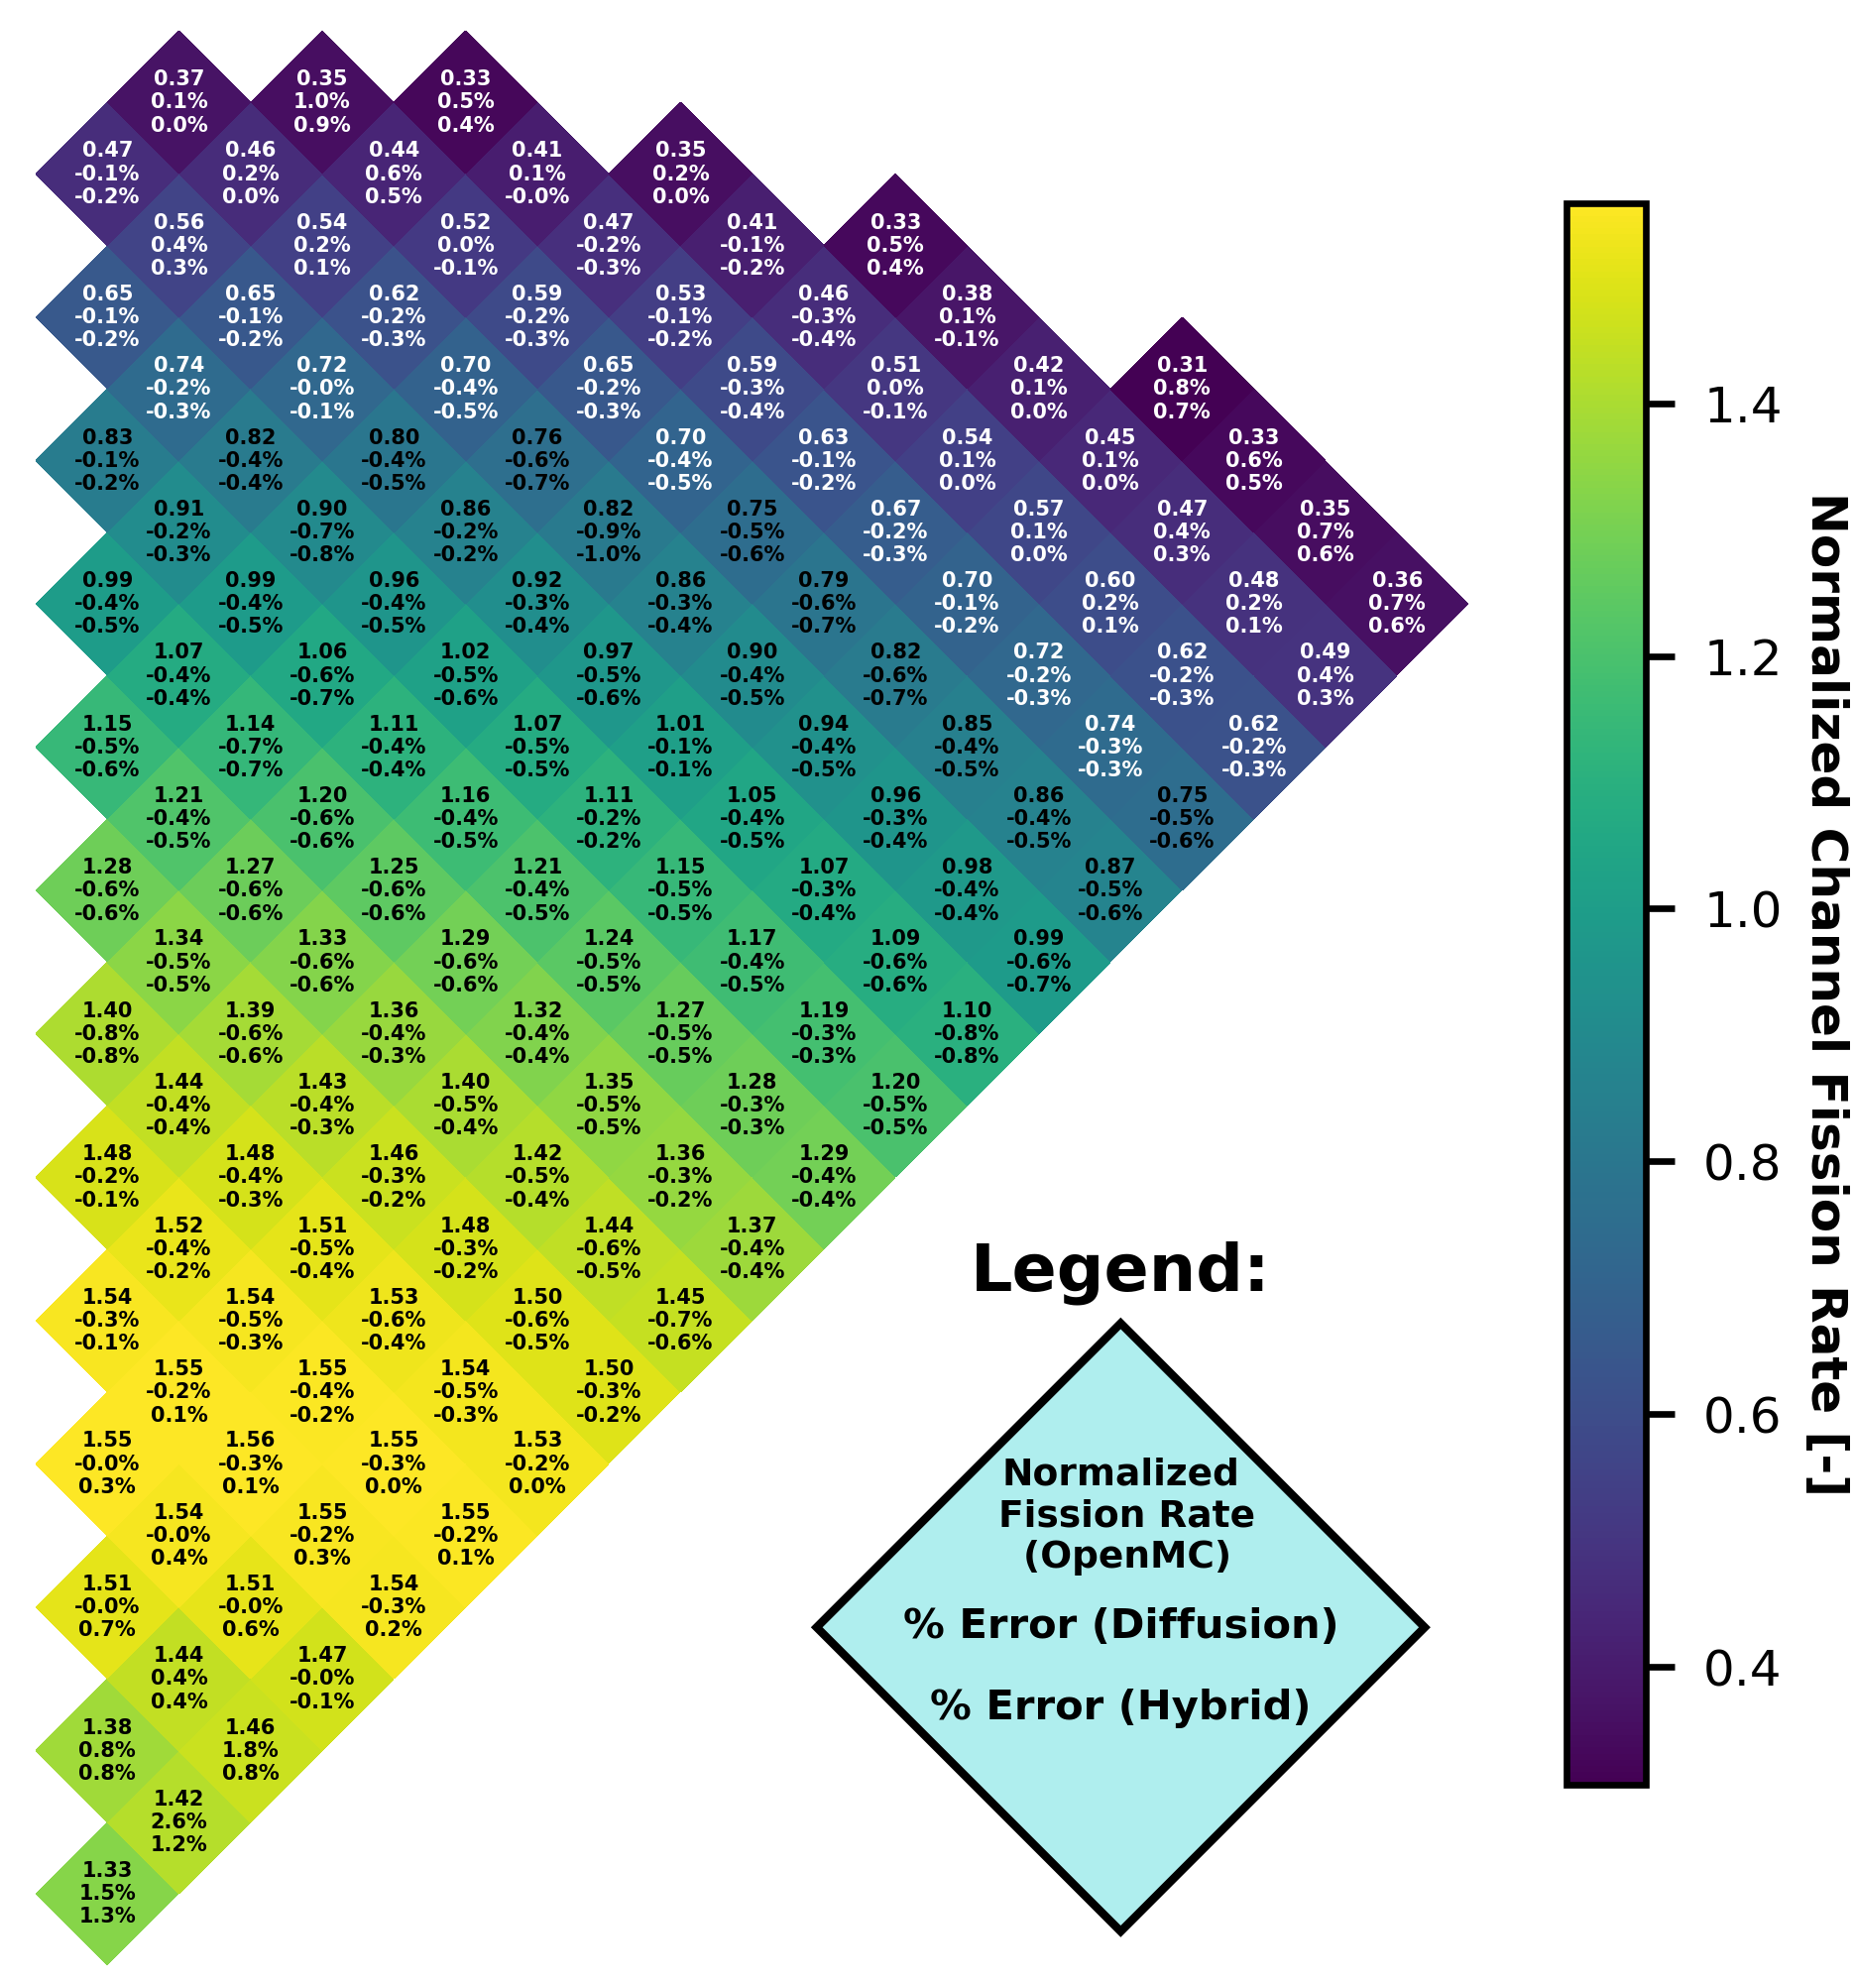
\includegraphics[width=\columnwidth]{msre-quarter-no-rod-power}
  \caption{Normalized channel fission rate distribution of the 2-D \gls{MSRE} quarter-core model
    with the rod withdrawn.
  This figure depicts the 1/8th-core distribution due to symmetry about the diagonal.}
  \label{fig:1/4-no-rod}
\end{figure}

\begin{figure}[p]
  \centering
  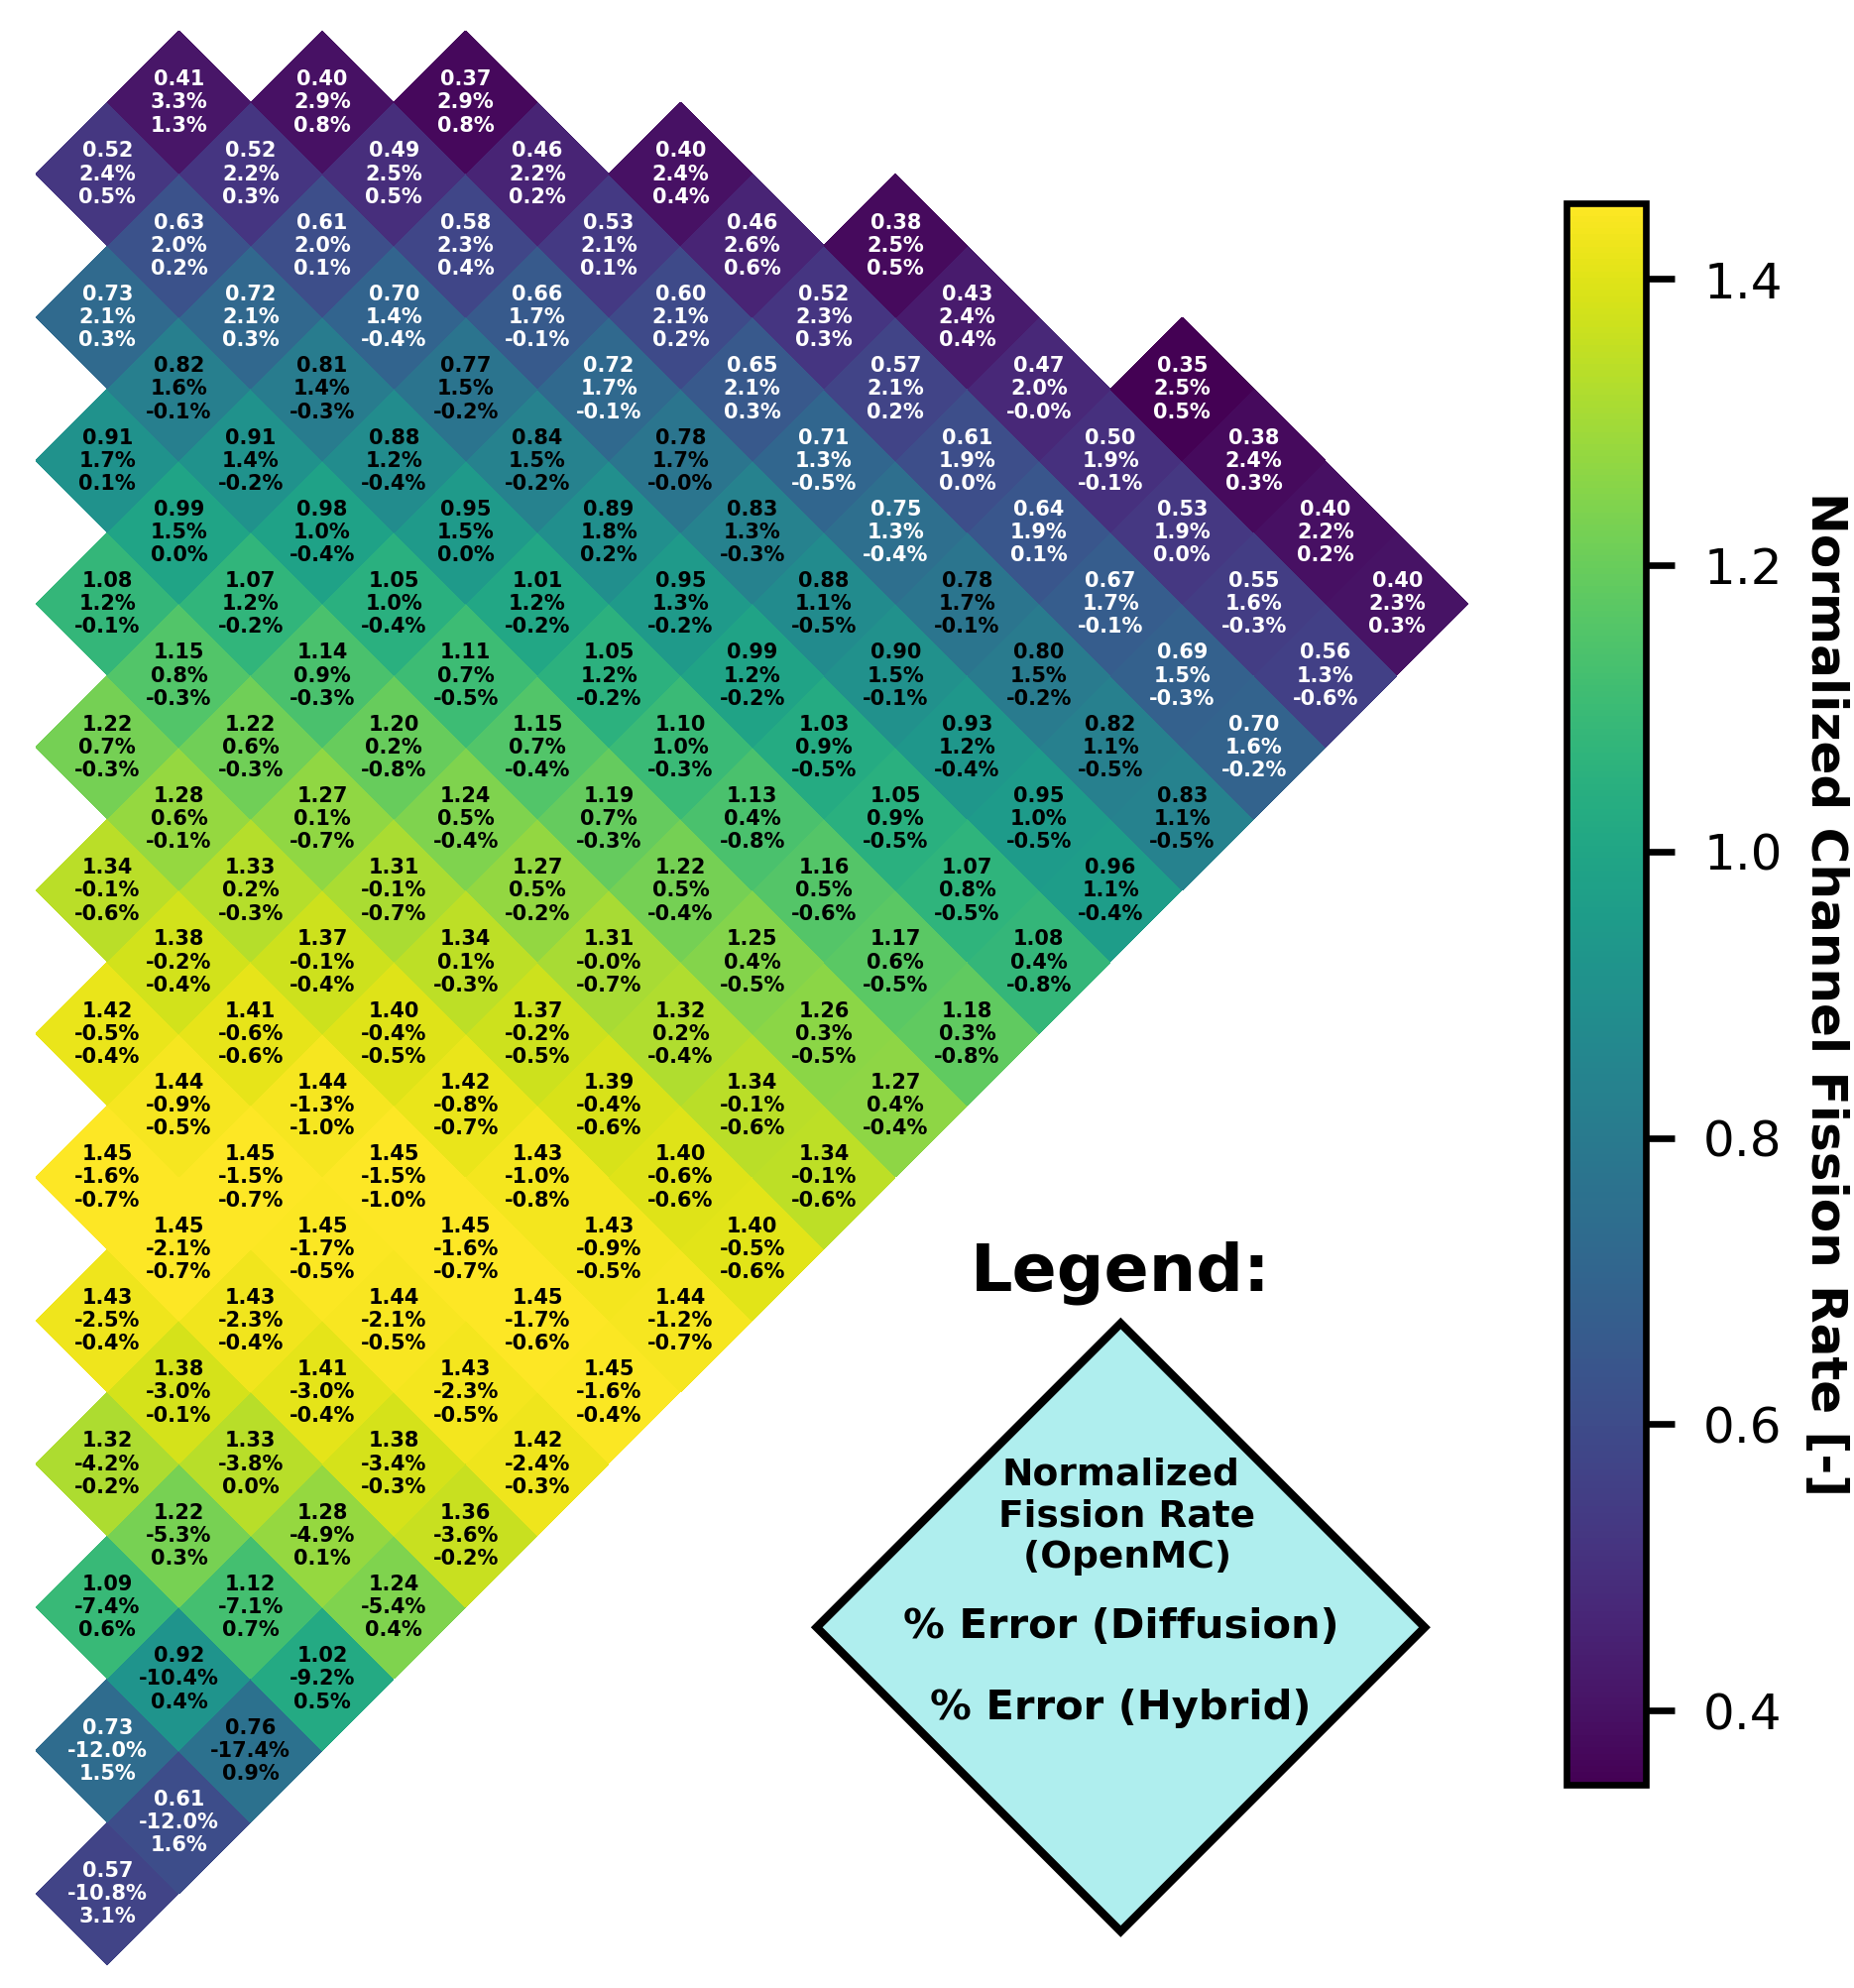
\includegraphics[width=\columnwidth]{msre-quarter-rod-power}
  \caption{Normalized channel fission rate distribution of the 2-D \gls{MSRE} quarter-core model
    with the rod inserted.
  This figure depicts the 1/8th-core distribution due to symmetry about the diagonal.}
  \label{fig:1/4-rod}
\end{figure}

\FloatBarrier

We calculated the normalized channel fission rate distribution by integrating the fission rate
within each fuel salt channel and normalizing the values such that the integrated fission rate in
each channel averages to 1 as follows
%
\begin{align}
  \text{Normalized fission rate of channel }i &= \frac{(\text{Total number of channels})\times
    (\text{Fission rate in channel }i)}{\text{Total fission rate in channels}} \nonumber \\
                                              &= \frac{N_i\sum^G_{g=1}\int_{V_i}\Sigma_{f,g}
  \phi_g(\vec{r}) dV}{
  \sum^{N_i}_{i=1}\sum^G_{g=1}\int_{V_i}\Sigma_{f,g}\phi_g(\vec{r}) dV}.
\end{align}
%
The total fission rate includes fission rate contributions from peripheral fuel salt regions.
Division by total fission rate normalizes the fission rates across the different neutronics
methods.
Figures \ref{fig:1/4-no-rod} and \ref{fig:1/4-rod} show the normalized fission rate distributions
of the quarter-core model for the ``No Rod'' and ``Rod'' cases, respectively. The figures present
1/8th slices of the core because the distributions are symmetrical about the $y=x$ line
outside of statistical variances for OpenMC-CE. The midpoints of fuel salt channels to form the
diamond lattice structure shown in the figures.
Each diamond element in the figures corresponds a horizontally or vertically oriented channel
depicted in Figure \ref{fig:1/4-geom}. The lattice also provides a guide for subdividing the
annular fuel regions around the control rod thimbles. The fission rate
distributions omit four channels along the outer edge due to the proximity to peripheral annular
fuel regions and the consequent difficulty in accurately tallying fission rates.

In the ``No Rod'' case, the peak channel fission rate occured several channels away from the
physical center of the reactor core. The presence of the empty (air-filled) rod thimble depressed
fission rates near the center. The neutron diffusion and hybrid methods report similar percentage
errors relative to OpenMC-CE except near the center. While the hybrid method benefits from drift
corrections, the neutron diffusion method's reliance on scalar diffusion coefficients tends to
artificially flatten neutron fluxes in near-void regions. Therefore, the largest percentage errors
from the neutron diffusion method occurred in the second and third diamond elements
diagonally up from the bottom which represent the annular fuel region surrounding the rod thimble.
In the ``Rod'' case, the introduction of the control rod shifted the peak further away from the
center as expected of a highly neutron-absorbing material. The rod further worsened fission rate
errors for the neutron diffusion method with errors of 1\% or more at the core center and
periphery. On the other hand, the fission rate errors for the hybrid method largely remained below
1\%.

\begin{table}[htb]
  \small
  \centering
  \caption{Absolute mean and maximum percentage errors in the normalized channel fission rates of
  the 2-D \gls{MSRE} quarter-core models relative to OpenMC. The mean relative standard deviation of
  OpenMC normalized channel fission rates is 0.20\%.}
  \begin{tabular}{l S S S S}
    \toprule
    \multirow{2}{*}{Method} & \multicolumn{2}{c}{No Rod} & \multicolumn{2}{c}{Rod} \\
                            & {Mean [\%]} & {Maximum [\%]} & {Mean [\%]} & {Maximum [\%]} \\
                            \cmidrule(r){1-1} \cmidrule(rl){2-3} \cmidrule(l){4-5}
    Diffusion & 0.40 & 2.63 & 2.01 & 17.44 \\
    Hybrid & 0.40 & 1.32 & 0.43 & 3.08 \\
    \bottomrule
  \end{tabular}
  \label{table:quarter-core-power}
\end{table}

Table \ref{table:quarter-core-power} shows the absolute mean and maximum percentage errors of the
normalized channel fission rates from the neutron diffusion and hybrid methods relative to
OpenMC-CE. Overall, the hybrid method reported smaller percentage errors than the neutron diffusion
method. The absolute maximum percentage error from the neutron diffusion method jumped to 17.44\%
as compared to 3.08\% for the hybrid method in the ``Rod'' case. Along with the figures, these
results demonstrate the hybrid method provides improved fission rate distribution accuracy in
the existence of near-void and highly neutron-absorbing regions.

\FloatBarrier

%\subsubsubsection{2-D Full-Core}

We performed the same $k_\text{eff}$ and fission rate distribution analyses with the 2-D full-core
model under four configurations starting from no rod inserted to all three rods inserted. The
$k_\text{eff}$ and error estimates in Table \ref{table:full-core-k} show the same trends observed
with the 2-D quarter-core model. OpenMC-MG and the hybrid method exhibit moderate but consistent
reactivity errors of approximately the 550 pcm and 800 pcm, respectively. The neutron diffusion
method reported errors ranging from 692 pcm when no rod is inserted to -470 pcm when all three rods
are inserted. Consequently, in Table \ref{table:full-core-worth}, OpenMC-MG and the hybrid method
report accurate control rod worths within 1-3 standard deviations of OpenMC-CE while the neutron
diffusion method increasingly overestimates the rod worth as more rods are inserted.

\begin{table}[htb]
  \small
  \centering
  \caption{$k_\text{eff}$ estimates for the 2-D full-core \gls{MSRE} model with the indicated rods
    inserted. Error values are relative to OpenMC-CE.}
  \setlength\tabcolsep{2pt}
  \begin{tabular}{l S[table-format=1.5(2)] S S[table-format=1.5(2)] S S[table-format=1.5(2)] S S[table-format=1.5(2)] S}
    \toprule
    \multirow{3}{*}{Method} & \multicolumn{2}{c}{No Rod} & \multicolumn{2}{c}{Rod 1} & \multicolumn{2}{c}{Rod 1 \& 2} & \multicolumn{2}{c}{Rod 1, 2 \& 3} \\
                            & {\multirow{2}{*}{$k_\text{eff}$}} & {Error} & {\multirow{2}{*}{$k_\text{eff}$}} & {Error} & {\multirow{2}{*}{$k_\text{eff}$}} & {Error} & {\multirow{2}{*}{$k_\text{eff}$}} & {Error} \\
                            & & {[pcm]} & & {[pcm]} & & {[pcm]} & & {[pcm]} \\
                            \cmidrule(r){1-1} \cmidrule(rl){2-3} \cmidrule(rl){4-5} \cmidrule(rl){6-7} \cmidrule(l){8-9}
    OpenMC-CE & 1.09859(20) & {-} & 1.06980(21) & {-} & 1.04690(18) & {-} & 1.02688(18) & {-} \\
    OpenMC-MG & 1.10637(19) & 640 & 1.07633(20) & 567 & 1.05235(20) & 495 & 1.03262(17) & 541 \\
    Diffusion & 1.10701 & 692 & 1.07120 & 122 & 1.04415 & -252 & 1.02195 & -470 \\
    Hybrid & 1.10843 & 808 & 1.07906 & 802 & 1.05553 & 781 & 1.03582 & 841 \\
    \bottomrule
  \end{tabular}
  \label{table:full-core-k}
\end{table}

\begin{table}[htb]
  \small
  \centering
  \caption{Control rod worth estimates for the 2-D full-core \gls{MSRE} with the
  indicated rods inserted. Error values are relative to OpenMC-CE.}
  \setlength\tabcolsep{5pt}
  \begin{tabular}{l S[table-format=4(2)] S S[table-format=4(2)] S S[table-format=4(2)] S}
    \toprule
    \multirow{2}{*}{Method} & \multicolumn{2}{c}{Rod 1} & \multicolumn{2}{c}{Rod 1 \& 2} & \multicolumn{2}{c}{Rod 1, 2 \& 3} \\
                            & {$\Delta\rho_\text{worth}$ [pcm]} & {Error [pcm]} & {$\Delta\rho_\text{worth}$ [pcm]} & {Error [pcm]} & {$\Delta\rho_\text{worth}$ [pcm]} & {Error [pcm]} \\
                            \cmidrule(r){1-1} \cmidrule(rl){2-3} \cmidrule(rl){4-5} \cmidrule(l){6-7}
    OpenMC-CE & 2450(25) & {-} & 4494(23) & {-} & 6357(24) & {-} \\
    OpenMC-MG & 2523(23) & 73 & 4640(24) & 146 & 6455(22) & 98 \\
    Diffusion & 3019 & 569 & 5439 & 945 & 7519 & 1162 \\
    Hybrid & 2455 & 5 & 4521 & 27 & 6323 & -34 \\
    \bottomrule
  \end{tabular}
  \label{table:full-core-worth}
\end{table}

Plots of the normalized channel fission rate distributions for all four rod configurations are
available in Appendix \ref{chap:2d-fiss-rate}. They are best viewed in digital pdf format with zoom
magnification due to the numerous fuel salt channels and small fonts.

Table \ref{table:full-core-power} shows the absolute mean and maximum percentage errors in the
normalized channel fission rates from the neutron diffusion and hybrid methods relative to
OpenMC-CE. Both mean and maximum percentage errors from the neutron diffusion method steadily
increase with the number of rods inserted. The mean percentage error from the hybrid method remains
constant at 0.43\% while the maximum percentage error increases marginally from 1.45\% to 2.52\%
when all three rods are inserted. These results demonstrate the hybrid method remains
effective at improving control rod worth and fission rate distribution estimates in geometries with
asymmetric rod configurations.

\begin{table}[htb]
  \footnotesize
  \centering
  \caption{Absolute mean and maximum percentage errors in the normalized channel fission rates of
  the 2-D \gls{MSRE} full-core models relative to OpenMC. The mean relative standard deviation of
  OpenMC normalized channel fission rates is 0.27\%.}
  \setlength\tabcolsep{2.5pt}
  \begin{tabular}{l S S S S S S S S}
    \toprule
    \multirow{2}{*}{Method} & \multicolumn{2}{c}{No Rod} & \multicolumn{2}{c}{Rod 1} & \multicolumn{2}{c}{Rod 1 \& 2} & \multicolumn{2}{c}{Rod 1, 2 \& 3} \\
                            & {Mean [\%]} & {Maximum [\%]} & {Mean [\%]} & {Maximum [\%]} & {Mean [\%]} & {Maximum [\%]} & {Mean [\%]} & {Maximum [\%]} \\
                            \cmidrule(r){1-1} \cmidrule(rl){2-3} \cmidrule(rl){4-5} \cmidrule(rl){6-7} \cmidrule(l){8-9}
    Diffusion & 0.45 & 2.95 & 0.94 & 12.61 & 1.35 & 15.34 & 1.67 & 17.09 \\
    Hybrid & 0.43 & 1.45 & 0.43 & 1.82 & 0.43 & 2.26 & 0.43 & 2.52 \\
    \bottomrule
  \end{tabular}
  \label{table:full-core-power}
\end{table}

\FloatBarrier

%\subsubsubsection{$S_N$ Discretization \& Ray Effects}

Angular resolution in 2-D (and later 3-D) flux simulations is important for accurately capturing
the angular dependence in the neutron angular flux. This subsection compares the $k_\text{eff}$ and
neutron scalar flux distribution solutions from the hybrid method with the $S_6$, $S_8$, $S_{10}$,
and $S_{12}$ methods for the 2-D full-core with no rods inserted. Table
\ref{table:2d-sn-convergence} shows the $k_\text{eff}$ estimates from those simulation results.
The $k_\text{eff}$ varies by less than 1 pcm, thereby indicating that the angular discretization
order used by the hybrid method has little impact on the integral reactor parameters.

Figures \ref{fig:ray-effect-12} and \ref{fig:ray-effect-34} show the first four neutron group flux
distributions from the hybrid method in the central reactor region consisting of three
air-filled thimbles and a homogenized sample basket (bottom right). The geometry corresponds
directly to Figure \ref{fig:full-geom-closeup} without the three control rods. Group 1 fluxes
in the thimble form a distinctive ray effect artifacts arising from the regular geometrical shapes and
insufficient angular resolution. The artifacts become less distinct with increasing angular
discretization levels. They also diminish with increasing neutron energy groups due to shorter
neutron mean free paths leading to more diffusive behavior.

By Group 3 and 4, the artifacts are indiscernible to the eye across all angular discretization
orders. Given that $k_\text{eff}$ is heavily weighted towards the later (slower) energy groups due
to larger fission cross sections, it is clear why Table \ref{table:2d-sn-convergence} shows little
differences in $k_\text{eff}$ across the angular discretization orders. Therefore, $S_8$ is
adequate for control rod worth calculations in the \gls{MSRE}. 
Further investigations into the angular discretization level may be warranted when applying the
hybrid method to reactors with more air-filled or highly-heterogeneous regions such as in
high-temperature gas-cooled reactors.

\begin{table}[t]
  \centering
  \caption{Hybrid method $k_\text{eff}$ estimates for the 2-D full-core model with zero rods
  inserted and $S_N$ schemes from $S_6$ to $S_{12}$.}
  \begin{tabular}{l S}
    \toprule
    Angular discretization & {$k_\text{eff}$} \\
    \midrule
    $S_6$ & 1.108414 \\
    $S_8$ & 1.108423 \\
    $S_{10}$ & 1.108422 \\
    $S_{12}$ & 1.108420 \\
    \bottomrule
  \end{tabular}
  \label{table:2d-sn-convergence}
\end{table}

\begin{figure}[p]
  \small
  \centering
  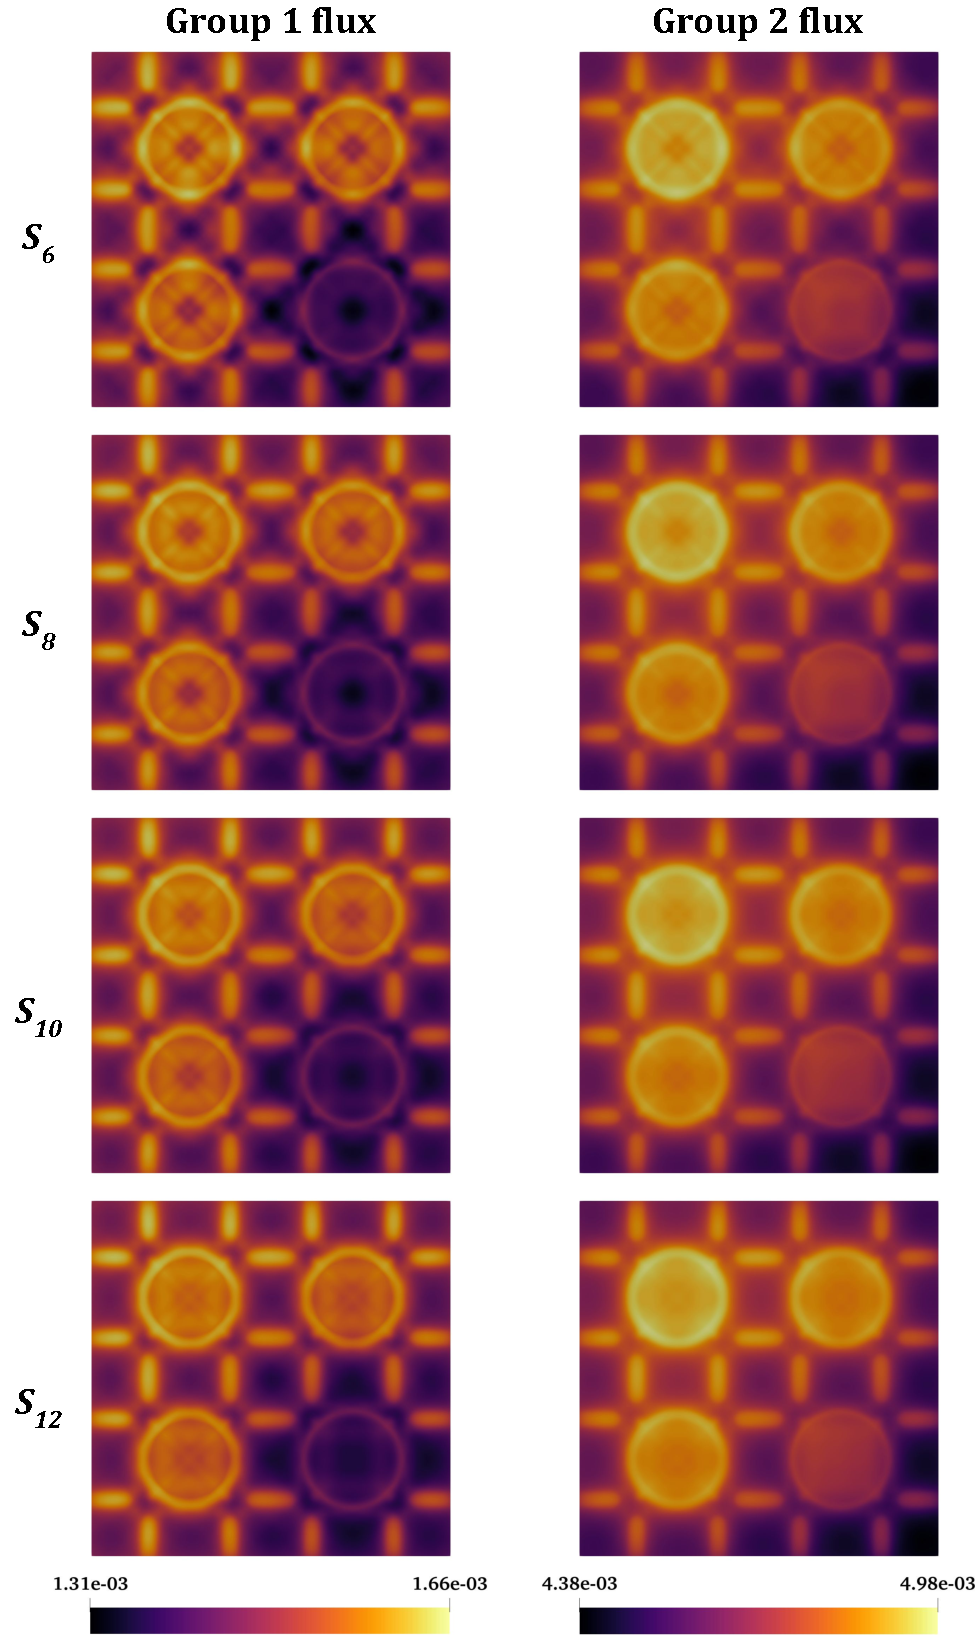
\includegraphics[width=0.7\columnwidth]{ray-effect-12}
  \caption{Group 1 and 2 neutron flux distributions in the hybrid $S_N$-diffusion method correction
  region with $S_6$, $S_8$, $S_{10}$, \& $S_{12}$. Ray effects diminish with increasing
  angular fidelity, but still persist with $S_{12}$ in group 1 and 2.}
  \label{fig:ray-effect-12}
\end{figure}

\begin{figure}[p]
  \small
  \centering
  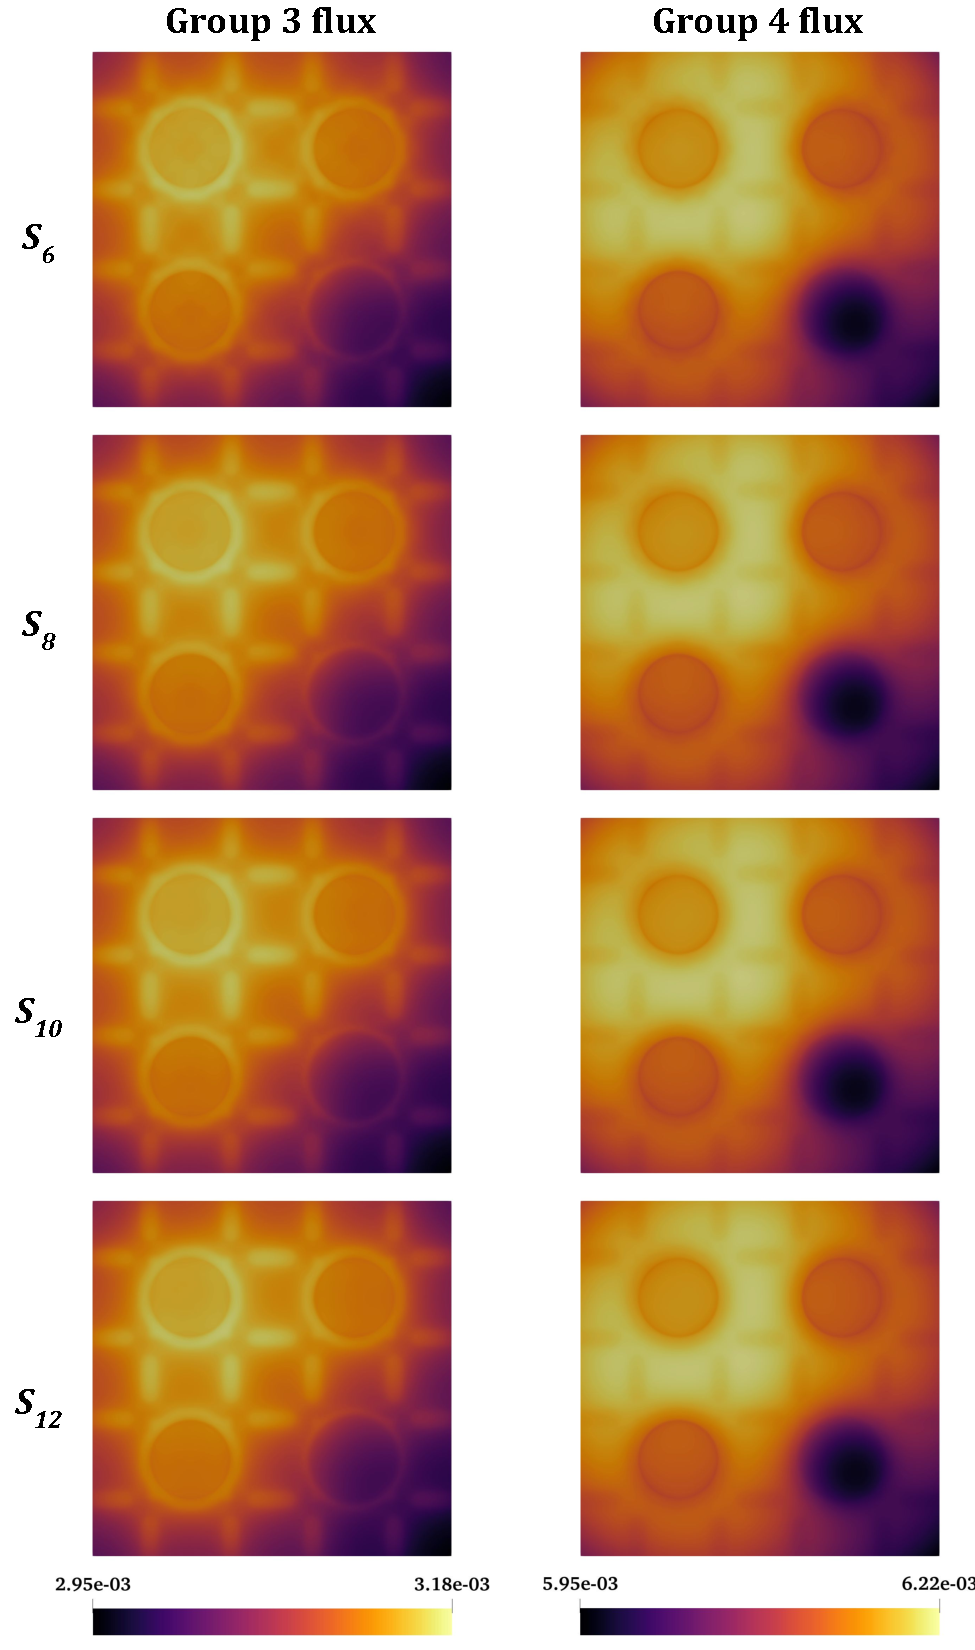
\includegraphics[width=0.7\columnwidth]{ray-effect-34}
  \caption{Group 3 and 4 neutron flux distributions in the hybrid $S_N$-diffusion method correction
  region with $S_6$, $S_8$, $S_{10}$, \& $S_{12}$. Ray effects are barely visible in group
  3 and 4 due to shorter neutron mean free paths.}
  \label{fig:ray-effect-34}
\end{figure}

%\subsection{3-D Neutronics Models \& Results} \label{sec:3d-results}
%
%This section presents the models, results, and discussion of the 3-D \gls{MSRE} simulations.
%Section \ref{sec:3d-model-setup} describes the model setup for the 3-D \gls{MSRE} simulations.
%Section \ref{sec:3d-nts} covers the results and discussion of the 3-D \gls{MSRE} simulations.
%
%\subsubsection{3-D Neutronics Model Setup} \label{sec:3d-model-setup}
%
%Figure \ref{fig:msre-picture} shows the vertical cross section of the actual \gls{MSRE} vessel.
%The actual design has rounded upper and lower plena to help direct salt flow through the system.
%This work uses a modified 3-D numerical \gls{MSRE} model as shown by Figures
%\ref{fig:msre-geom-vert} and \ref{fig:wedge-view}. The model excludes the toroidal flow distributor
%near the top
%of the vessel and reshapes the plena into right cylinders. It has the same horizontal cross section
%as the 2-D model (Figure \ref{fig:full-geom}) throughout most of the salt-graphite lattice. In
%addition to modifications in the 2-D model listed in Section \ref{sec:2d-model-setup}, the
%3-D model includes the following modifications:
%
%\begin{itemize}
%  \item Removed the toroidal flow distributor near the top of the vessel.
%  \item Reshaped the upper and lower plena into right cylinders while keeping the salt volume
%    constant.
%  \item Flattened the conical tops of the graphite lattice blocks.
%  \item Regularized the complicated graphite lattice structure at the bottom.
%  \item Set a fixed outer vessel thickness of 2.54 cm.
%  \item Homogenized the lower plenum by 90.8\% salt-9.2\% INOR-8 (vessel) by volume.
%  \item Removed the reactor access nozzle and the various components within it.
%  \item Added a graphite block at the bottom of the control rod thimbles.
%\end{itemize}
%
%\begin{figure}[p]
%  \centering
%  \includegraphics[width=0.97\columnwidth]{msre-picture}
%  \caption{Vertical cross section of the actual \gls{MSRE} vessel \cite{robertson_msre_1965}.
%  It has rounded upper and lower
%  plena, and a toroidal flow distributor that distributes the salt inflow evenly as it enters the
%  core through holes on the inside vessel surface of the distributor.}
%  \label{fig:msre-picture}
%\end{figure}
%
%\begin{figure}[p]
%  \centering
%  \includegraphics[width=\columnwidth]{msre-geom-vert}
%  \caption{Vertical cross section of the 3-D numerical \gls{MSRE} model offset by 5.08 cm to show
%  the control rod thimble and homogenized sample basket. The control rod is in its fully inserted
%  position. The homogenized lower plenum consists of 90.8\% salt and 9.2\% INOR-8 alloy by volume.}
%  \label{fig:msre-geom-vert}
%\end{figure}
%
%\begin{figure}[p]
%  \centering
%  \includegraphics[width=\columnwidth]{wedge-view-high-res}
%  \caption{3-D section view of the 3-D numerical \gls{MSRE} model offset by 5.08 cm in the $x$ and
%  $y$ axes to show the three control rod thimbles. Rod 1 is inserted by 4.4 inches while Rods 2 \&
%  3 are fully withdrawn.}
%  \label{fig:wedge-view}
%\end{figure}
%
%Table \ref{table:reactor-dimensions} lists relevant dimensions of the 3-D \gls{MSRE} model.
%All material compositions remain
%the same as the 2-D models and the \gls{MSRE} benchmark specifications \cite{fratoni_molten_2020}.
%All 3-D neutronics simulations in this section used the molten salt composition with 65.25 kg
%$^{235}$U loaded (Table \ref{table:2d-salt-composition}), except the simulations for temperature
%reactivity coefficient calculations which had a higher $^{235}$U loading of 67.00 kg (Table
%\ref{table:67-salt-composition}).
%
%\begin{table}[htb]
%  \centering
%  \caption{List of key dimensions of the 3-D \gls{MSRE} model used in this work.}
%  \begin{tabular}{l S}
%    \toprule
%    Reactor Specifications & {Value} \\
%    \midrule
%    Total height [cm] & 215.5967 \\
%    Lower plenum height [cm] & 18.7530 \\
%    Upper plenum height [cm] & 25.3937 \\
%    Total radius [cm] & 76.200 \\
%    Graphite core radius [cm] & 70.168 \\
%    Core can inner radius [cm] & 70.485 \\
%    Core can outer radius [cm] & 71.120 \\
%    Vessel thickness [cm] & 2.540 \\
%    Fuel channel length [cm] & 3.048 \\
%    Fuel channel width [cm] & 1.016 \\
%    Graphite lattice pitch [cm] & 5.080 \\
%    Control rod inner radius [cm] & 1.0668 \\
%    Control rod outer radius [cm] & 1.3716 \\
%    Control rod thimble inner radius [cm] & 2.3749 \\
%    Control rod thimble outer radius [cm] & 2.540 \\
%    Homogenized sample basket radius [cm] & 2.8575 \\
%    Radius of fuel annulus around thimble [cm] & 3.2016 \\
%    \bottomrule
%  \end{tabular}
%  \label{table:reactor-dimensions}
%\end{table}
%
%\begin{table}[htb]
%  \small
%  \centering
%  \setlength\tabcolsep{4pt}
%  \caption{\gls{MSRE} molten salt composition when the $^{235}$U loading was at 65.25 kg.}
%  \begin{tabular}{l S S S S S S S}
%    \toprule
%    Element & {Li} & {Be} & {Zr} & {Hf} & {$^{234}$U} & {$^{235}$U} & {$^{236}$U} \\
%    \midrule
%    Composition [kg] & 507.42 & 293.96 & 513.97 & 0.0029 & 0.68 & 67.00 & 0.28 \\
%    \bottomrule
%  \end{tabular}
%  \begin{tabular}{l S S S S S S}
%    \toprule
%    Element & {$^{238}$U} & {Fe} & {Cr} & {Ni} & {O} & {F} \\
%    \midrule
%    Composition [kg] & 142.02 & 0.75 & 0.13 & 0.14 & 2.27 & 3104.22 \\
%    \bottomrule
%  \end{tabular}
%  \label{table:67-salt-composition}
%\end{table}
%
%All neutronics simulations ran on OpenMC under continuous energy mode and on Moltres with the
%hybrid $S_N$-diffusion method. The hybrid simulations ran with a maximum stabilization factor of
%$c=250$, a void constant of $\varsigma=0.5$, and a uncorrected diffusion coefficient cap of $D_g=2.5$.
%Refer to Sections \ref{sec:void-treatment} and \ref{sec:diffcoef-cap} for the relevant discussion
%on void treatment for near-void regions and the impact of large diffusion coefficient values on
%solver performance. As for the standard neutron diffusion method, it either converges very slowly
%or does not converge at all when $D_g$ values are uncapped due to excessive diffusive effects in
%the air-filled control rod thimbles. Group-wise $D_g$ values, generated using OpenMC, ranged from
%100 cm to 850 cm in the air regions as compared to the typical 0.5 cm to 2.0 cm range observed in
%non-air regions. Therefore, all neutron diffusion method simulation results in the following
%section were measured with the diffusion coefficient capped at $D_g=2.5$.
%
%Unlike the 2-D hybrid simulations which ran with $S_8$ angular discretization, the 3-D hybrid
%simulations ran with $S_6$ angular discretization due to significantly
%larger computational and memory requirements demanded by the 3-D simulations. Further discussion on
%computational performance may be found at the end of Section \ref{sec:3d-nts}. All simulations,
%except those for temperature reactivity coefficient calculations, ran on isothermal 3-D models at
%911 K.
%
%\begin{table}[htb]
%  \small
%  \centering
%  \setlength\tabcolsep{4pt}
%  \caption{Axial discretization of the 3-D \gls{MSRE} model mesh.}
%  \begin{tabular}{l S S S S}
%    \toprule
%    Layer & {Layer height [cm]} & {Layer start height [cm]} & {Layer end height [cm]} & {Layer mesh resolution} \\
%    \midrule
%    1 & 2.5400 & 0.0000 & 2.5400 & 1 \\
%    2 & 18.7530 & 2.5400 & 21.2930 & 4 \\
%    3 & 5.0800 & 21.2930 & 26.3730 & 1 \\
%    4 & 14.6050 & 26.3730 & 40.9780 & 3 \\
%    5 & 139.7000 & 40.9780 & 180.6780 & 28 \\
%    6 & 6.9850 & 180.6780 & 187.6630 & 2 \\
%    7 & 25.3937 & 187.6630 & 213.0567 & 5 \\
%    8 & 2.5400 & 213.0567 & 215.5967 & 1 \\
%    \bottomrule
%  \end{tabular}
%  \label{table:axial-mesh}
%\end{table}
%
%\subsubsection{3-D Numerical Results \& Discussion} \label{sec:3d-nts}
%
%%\subsubsubsection{Initial Criticality Configuration}
%
%The \gls{MSRE} achieved initial criticality with Rod 1 inserted to a height of 46.6 inches relative
%to the fully inserted position. For reference, the rods are at a height of 51 inches when fully
%withdrawn. Table \ref{table:initial-crit} shows the $k_\text{eff}$ values from \gls{MSRE}
%experimental data, numerical benchmark data \cite{fratoni_molten_2020}, and this work. All
%numerical models overestimate the $k_\text{eff}$ relative to the experimental value by 1-2\%
%(1000-2000 pcm). In the \gls{MSRE} numerical benchmark report, the authors
%attribute this $k_\text{eff}$ discrepancy largely to discrepancies in the carbon cross section data
%in nuclear data libraries. They noted similar $k_\text{eff}$ overestimations by 1-2\% in benchmark
%results for the HTTR, a graphite-moderated, helium-cooled reactor. The OpenMC and Moltres
%simulations in this work used the same
%ENDF/B-VII.1 nuclear data library as the \gls{MSRE} numerical benchmark report.
%
%\begin{table}[htb]
%  \centering
%  \caption{$k_\text{eff}$ values from \gls{MSRE} experimental data, the \gls{MSRE} numerical
%  benchmark \cite{fratoni_molten_2020}, and the OpenMC and Moltres models in this work.}
%  \begin{tabular}{l S[table-format=1.5(2)]}
%    \toprule
%     & {$k_\text{eff}$} \\
%     \midrule
%    \gls{MSRE} experimental data & 1.00000(420) \\
%    Serpent 2 (Numerical benchmark) & 1.02132(3) \\
%    OpenMC (This work) & 1.01308(20) \\
%    Hybrid (This work) & 1.01955 \\
%    Diffusion (This work) & 1.01885 \\
%    \bottomrule
%  \end{tabular}
%  \label{table:initial-crit}
%\end{table}
%
%Of the four $k_\text{eff}$ values, we expect to see the closest agreement between the Serpent 2
%model from the numerical benchmark and OpenMC from this work. However, the OpenMC \gls{MSRE} model
%differs from the Serpent 2 \gls{MSRE} models due to geometry modifications listed in Sections
%\ref{sec:2d-model-setup} and \ref{sec:3d-model-setup}. The benchmark report quantified the impact
%of several geometry modifications, namely the removal of the flow distributor, the homogenization
%of the sample basket, and the removal of the thermal shield. These modifications contribute to
%-$0.098\%$, -$0.037\%$, and -$0.885\%$ change in the $k_\text{eff}$, respectively, for an overall
%$k_\text{eff}$ estimate of $1.01093(3)$. This brings the OpenMC $k_\text{eff}$ estimate of
%$1.01308(20)$ to closer agreement with the numerical benchmark value.
%
%The hybrid method $k_\text{eff}$ estimate is 0.00647 higher than the OpenMC estimate. For this
%initial criticality configuration, the neutron diffusion method $k_\text{eff}$ estimate is closer
%to OpenMC than the hybrid method. Overall, the OpenMC and Moltres models show good agreement with
%the Serpent 2 model from the numerical benchmark.
%
%Figures \ref{fig:3d-view}, \ref{fig:ic-g1}, and \ref{fig:ic-g8} show a 3-D section view of the
%\gls{MSRE} model geometry and the group 1 \& 8 neutron
%flux distributions. The salt-graphite lattice structure is visible from the group flux
%distributions. The group 1 flux distribution largely retains a spherical shape. The group 8 neutron
%flux distribution is particularly suppressed near the control rods due to strong thermal neutron
%capture cross section of gadolinium.
%
%\begin{figure}[p]
%  \centering
%  \includegraphics[width=\columnwidth]{3d-view-high-res}
%  \caption{3-D section view of the \gls{MSRE} model geometry with Rod 1 inserted by 4.4 inches at
%  initial criticality.}
%  \label{fig:3d-view}
%\end{figure}
%
%\begin{figure}[p]
%  \centering
%  \includegraphics[width=\columnwidth]{ic-g1}
%  \caption{Group 1 neutron flux distribution with Rod 1 inserted by 4.4 inches at initial
%  criticality.}
%  \label{fig:ic-g1}
%\end{figure}
%
%\begin{figure}[p]
%  \centering
%  \includegraphics[width=\columnwidth]{ic-g8}
%  \caption{Group 8 neutron flux distribution with Rod 1 inserted by 4.4 inches at initial
%  criticality.}
%  \label{fig:ic-g8}
%\end{figure}
%
%%\subsubsubsection{Control Rod Worth}
%
%After achieving initial criticality, \gls{MSRE} researchers ran control rod calibration experiments
%with the \gls{MSRE} at zero-power (typically at about 10 W power output)
%\cite{prince_zero-power_1968}. They measured differential rod worths by measuring the time taken
%for the reactor power to increase by 20 W following a prescribed withdrawal of Rod 1 and applying
%the inhour equation to obtain the reactivity inserted. They repeated this process at different rod
%heights after successive additions of highly enriched uranium capsules. The final integral rod
%worth curve was normalized to the critical $^{235}$U loading of 65.25 kg
%\cite{prince_zero-power_1968}.
%
%For control rod worth calculations, the OpenMC and Moltres simulations ran with Rod 1 at fourteen
%different rod positions from full insertion (0 inch) to full withdrawal (51 inches). The rod
%positional limits of 0 inch and 51 inches represents the full range of deliberate rod motion
%allowable by the control rod drive motor \cite{robertson_msre_1965}.
%
%Figure \ref{fig:rod-worth} shows the integral rod worth curves from the \gls{MSRE} experimental
%data and the OpenMC and Moltres numerical models. By taking the $k_\text{eff}$ when Rod 1 is fully
%inserted as reference, all rod worth curves start at 0 pcm. The change in integral rod worth,
%represented by the gradient in the plot, is steepest as the tip of the rod passes through the
%center of the core. The hybrid method performs well in reproducing the rod worth curve from OpenMC;
%all hybrid method rod worth values fall within one or two standard deviations of OpenMC.
%
%Due to the experimental procedure of computing integral rod worth through cumulative differential
%rod worth measurements, the uncertainty range of the \gls{MSRE} data scales with rod position.
%Both OpenMC and the hybrid method report consistently larger integral rod worths than the
%\gls{MSRE} data across all rod positions. Nevertheless, they are in good agreement with the
%\gls{MSRE} data as compared to the neutron diffusion method, which significantly overestimates the
%integral rod worth.
%Table \ref{table:rod-worth} shows the total rod worth of Rod 1. Similar to observations from Figure
%\ref{fig:rod-worth}, OpenMC and the hybrid method report total rod worths marginally larger than
%the \gls{MSRE} data by 5.1\% and 4.2\%, respectively, while the diffusion method exceeds the
%experimental value by 21.1\%.
%
%\begin{figure}[t]
%  \centering
%  \includegraphics[width=0.8\columnwidth]{rod-worth-curve}
%  \caption{Reactivity inserted by Rod 1 at various rod positions relative to the full insertion.}
%  \label{fig:rod-worth}
%\end{figure}
%
%\begin{table}[t]
%  \centering
%  \caption{Total rod worth of Rod 1 when fully inserted.}
%  \begin{tabular}{l S[table-format=4(2)] S}
%    \toprule
%     & {$\rho_\text{worth}$ [pcm]} & {Percentage discrepancy [\%]}\\
%     \cmidrule(rl){2-2} \cmidrule(l){3-3}
%    \gls{MSRE} experimental data & 2250(67) & {-}\\
%    OpenMC (This work) & 2364(44) & 5.1 \\
%    Hybrid (This work) & 2345 & 4.2 \\
%    Diffusion (This work) & 2725 & 21.1 \\
%    \bottomrule
%  \end{tabular}
%  \label{table:rod-worth}
%\end{table}
%
%The most likely factor for OpenMC and the hybrid method overpredicting the control rod worth is the
%modeling of control rods as individual annular cylinders as opposed to 36 separate control elements
%strung along a flexible stainless steel cable. Figure \ref{fig:rod-bead} depicts a poison element
%and its physical dimensions. Other than the Gd$_2$O$_3$-Al$_2$O$_3$ poison material, each control
%element has a top and bottom closure made of INOR-8 alloy. According to the physical dimensions,
%the closures make up 15.1\% of the total element height. The 3-D numerical \gls{MSRE} model in this
%work omits the outer and inner INOR-8 cladding and the flexible stainless cable, and replaces the
%top and bottom closure with poison material. Fully resolving the closures in Moltres would require
%excessively fine axial mesh resolution and advanced adaptive meshing features not currently
%available. A straightforward corrective measure for future \gls{MSRE} simulations would be to
%retain the solid annular cylinder structure and adjust the rod dimensions or the rod material
%composition to match the expected worth from \gls{MSRE} data or OpenMC simulations with the beaded
%geometry.
%
%\begin{figure}[t]
%  \begin{subfigure}[b]{0.33\columnwidth}
%    \centering
%    \includegraphics[width=\columnwidth]{rod-bead-2}
%  \end{subfigure}
%  \begin{subfigure}[b]{0.65\columnwidth}
%    \centering
%    \includegraphics[width=\columnwidth]{rod-bead}
%  \end{subfigure}
%  \caption{Cutaway view and dimensions of a control rod poison element. Retrieved from
%  \cite{tolson_msre_1967} and \cite{robertson_msre_1965}.}
%  \label{fig:rod-bead}
%\end{figure}
%
%Overall, the results show that the hybrid $S_N$-diffusion method accurately reproduces the control
%rod worth at various levels of insertion. As observed in the 1-D and 2-D models, the 3-D model
%$k_\text{eff}$ values exhibit some discrepancies relative to OpenMC, but the discrepancies do not
%affect rod worth estimates which are calculated as reactivity changes. This \gls{MSRE} hybrid model
%may be improved in future work by characterizing and applying neutron albedo at the vacuum
%boundaries.
%
%%\subsubsubsection{Temperature Reactivity Coefficient} \label{sec:temp-coef}
%
%This work compares isothermal temperature reactivity coefficients calculated from $k_\text{eff}$
%values measured at 872 K and 972 K with 67.86 $^{235}$U loading. This approach is identical to that
%of the \gls{MSRE} experimental measurements \cite{prince_zero-power_1968} and the \gls{MSRE}
%numerical benchmark calculations \cite{fratoni_molten_2020}. The temperature reactivity coefficient
%is calculated by dividing the difference in reactivities by the temperature change (100 K). All
%simulations included the effects of thermal expansion on the material density but left all reactor
%physical dimensions unchanged.
%
%\begin{table}[h]
%  \small
%  \centering
%  \caption{Isothermal temperature reactivity coefficients with 67.86 kg $^{235}$U loading from
%  \gls{MSRE} data, the \gls{MSRE} numerical benchmark \cite{fratoni_molten_2020}, and the OpenMC
%  and Moltres models in this work.}
%  \begin{tabular}{l S[separate-uncertainty=true,table-format=2.2(2)] S}
%    \toprule
%     & {Temperature coefficient [pcm K$^{-1}$]} & {Percentage discrepancy [\%]}\\
%     \cmidrule(rl){2-2} \cmidrule(l){3-3}
%    \gls{MSRE} experimental data & 13.41(150) & {-}\\
%    Serpent 2 (Numerical benchmark) & 12.51(23) & -6.7 \\
%    OpenMC (This work) & 13.85(43) & 3.3 \\
%    Hybrid (This work) & 13.98 & 4.3 \\
%    Diffusion (This work) & 14.01 & 4.5 \\
%    \bottomrule
%  \end{tabular}
%  \label{table:temp-coef}
%\end{table}
%
%Table \ref{table:temp-coef} compares the isothermal reactivity coefficients from the experimental
%and numerical sources. The OpenMC and Moltres models in this work show closer agreement with the
%\gls{MSRE} data than the Serpent 2 model from the \gls{MSRE} numerical benchmark. All numerical
%results fall within one standard deviation of the \gls{MSRE} data.
%
%%\subsubsubsection{Computational Performance}
%
%Beyond demonstrating the hybrid $S_N$-diffusion method, its computational performance is of
%interest as a candidate for time-dependent 3-D reactor simulations. All simulations ran on the
%Polaris supercomputer system at \gls{ANL}. Each compute node consists of a 2.8-GHz AMD EPYC Milan
%7543P 32-core CPU, four NVIDIA A100 GPUs, and 512 GB of RAM. The GPUs were not utilized in this
%work. Moltres uses the \gls{MPI} communication protocol for parallelizing simulations. For this
%work, simulations ran with 1-to-1 ratio of \gls{MPI} ranks to processor cores (i.e., 32 \gls{MPI}
%ranks per compute node).
%
%Every 3-D hybrid method $k$-eigenvalue
%simulation of the \gls{MSRE} consisted of 750M \glspl{DOF} and 1.69B \glspl{DOF} for
%% 747,688,760 \glspl{DOF} and 1,690,777,728 \glspl{DOF} for
%the neutron diffusion and $S_N$ subsolvers, respectively. Each \gls{DOF} corresponds to a scalar
%or angular group flux variable value defined at a mesh node. Each simulation ran with the distributed
%mesh feature, which partitions and distributes the mesh across however many \gls{MPI} ranks used
%in the simulation. All variable and mesh-linked data are also distributed with the mesh. This
%greatly reduces memory requirements compared to storing the full mesh for each \gls{MPI} rank.
%Each 3-D \gls{MSRE} simulation required at least forty nodes for sufficient memory to run. This
%sets a strict minimum requirement for the 3-D hybrid simulations. A significant fraction of
%memory use in Moltres comes from storing the residual and Jacobian quantities at each \gls{FEM}
%quadrature point. Given that terms in the $S_N$ equations share the same Jacobian formulation
%across all ordinate directions, memory use (and compute time) could be optimized by reducing
%duplicate Jacobian evaluations.
%
%On forty nodes, each full-core rod worth simulation
%required approximately 2.2 h to complete for a total of 88 node-hours or 2816 core-hours. The
%distributed mesh capability comes with the cost of increased data transfer times between the $S_N$
%and diffusion solvers due to increased inter-processor data transfers. Transfers accounted for
%approximately 0.675 h or 30 \% of the total simulation time. Future research into optimizing mesh
%distribution and transfer-related data caching may help to minimize data transfers and speed up
%hybrid method simulations. The solution time for the initial neutron diffusion calculation with zero
%drift correction also takes up approximately 30 \% of the total simulation time. After taking into
%consideration the computational cost of evaluating the drift term, the hybrid method
%requires about four times the solution time of the standard neutron diffusion method.
%
%\begin{figure}[t]
%  \centering
%  \begin{subfigure}[b]{0.49\columnwidth}
%    \centering
%    \includegraphics[width=\columnwidth]{scaling-total}
%    \caption{Total wall time}
%  \end{subfigure} \\
%  \begin{subfigure}[b]{0.49\columnwidth}
%    \centering
%    \includegraphics[width=\columnwidth]{scaling-solver}
%    \caption{Solver wall time}
%  \end{subfigure}
%  \begin{subfigure}[b]{0.49\columnwidth}
%    \centering
%    \includegraphics[width=\columnwidth]{scaling-transfer}
%    \caption{Transfer wall time}
%  \end{subfigure}
%  \caption{The total, solver, and transfer wall time of hybrid method simulations of the 3-D
%  quarter-core model on 10, 20, 40, and 80 compute nodes (32 processors per node) of the Polaris
%  supercomputer. The solver
%  time scales almost linearly ($q=0.8$) with the number of processors, while the transfer time
%  scales poorly with an increase in wall time at 80 nodes. All axes are in log scale.}
%  \label{fig:scaling}
%\end{figure}
%
%3-D simulations generally required more nonlinear iterations than 2-D simulations for the neutron
%diffusion subsolver to
%converge. This is likely due to increased streaming effects in 3-D air regions and the
%consequent poor performance of the Hypre-BoomerAMG preconditioning method. The performance of this
%preconditioner worsens with strong advective effects from the drift correction term. Thus,
%alternative preconditioning methods suited for advection-dominated problems may help accelerate
%the hybrid method.
%
%For the hybrid method to be viable for large time-dependent simulations, it must scale reasonably
%well on computing clusters. For this work, I investigated strong scaling, which measures how the
%solution time decreases when more cores are used while keeping the problem size fixed. This strong
%scaling study used 3-D quarter-core models run on 10, 20, 40, and 80 compute nodes.
%Figure \ref{fig:scaling} shows the results of this scaling study. The total wall time scales at a
%sublinear rate of approximately $q=0.7$. The total wall time is broken down into two components:
%the solver wall time (i.e., initialization, numerical solver, etc.) and the transfer time (i.e,
%data transfer between the $S_N$ and diffusion solvers). The solver wall time scales at a sublinear
%rate of approximately $q=0.8$, while the transfer wall time scales at approximately $q=0.6$ from
%ten to forty nodes before registering a wall time increase when going from forty nodes to eighty nodes.
%It is likely that the increase in inter-processor data transfers due to increased data distribution
%outweighed the increase in computational power when running the problem with more compute nodes.
%Further investigation is necessary to confirm this hypothesis.
%
%Nevertheless, the total wall time exhibits decent strong scaling performance. For Moltres
%simulations in the next chapter, I optimized the data transfer setup which reduced the
%proportion of transfer wall time in the total wall time to approximately 18 \%. Therefore, the total
%wall times would scale closer to the $q=0.8$ rate observed with solver wall times.
%This is a promising indication that the hybrid method would scale well for the modeling of larger
%reactor analyses.

%\FloatBarrier

%\subsection{Summary}
%
%This chapter covers work demonstrating the hybrid $S_N$-diffusion method implemented in Moltres
%through 1-D, 2-D, and 3-D $k$-eigenvalue simulations of \gls{MSRE} models. The hybrid method
%combines stengths of the $S_N$
%and diffusion methods by applying transport corrections generated using the high-fidelity $S_N$
%method near control rods while treating the rest of the problem with the lower-fidelity diffusion
%method for tractable time-dependent 3-D reactor analyses. This is achieved by identifying and
%setting up a subregion containing the control rod and its vicinity for $S_N$ transport
%calculations. The $S_N$ and diffusion solvers are coupled through boundary sources at the subregion
%boundaries. The hybrid method applies an adaptive algorithm for discarding inaccurate transport
%correction values near the subregion boundaries and preserving the smoothness of the neutron flux
%gradient. In this chapter, the 1-D simulations provided verification of the hybrid method for
%estimating control rod worth. The simulations also compared two different implementations of the
%hybrid method which differed by the use of drift or diffusion correction schemes.
%The 2-D and 3-D simulations extended the hybrid method to multi-dimensional problems. Additionally,
%the 3-D simulations validated the numerical \gls{MSRE} model against \gls{MSRE} experimental data
%and provided useful insight on the computational performance of the hybrid method for
%large reactor analyses.
%
%Six 1-D test cases based on the \gls{MSRE} with increasing geometric complexity were run using the
%standard $S_N$ method, the hybrid method, and standard neutron diffusion method and verified against
%reference OpenMC Monte Carlo neutron transport simulations under continuous neutron energy (OpenMC-CE) and
%multigroup (OpenMC-MG) modes. The $S_N$ implementation with nonlinear diffusion acceleration
%showed good agreement with OpenMC-MG which indicated that discrepancies between those codes and
%OpenMC-CE largely arose from the eight neutron energy group structure for multigroup simulations.
%Both hybrid method implementations, with drift or diffusion correction schemes, showed similar
%performance in the 1-D cases. While the $k_\text{eff}$ estimates from the hybrid method deviated
%from the $S_N$ method and OpenMC-MG by 100 to 400 pcm, the hybrid method accurately reproduces
%control rod worths. Rod worth estimates from OpenMC-MG, $S_N$, and hybrid methods differed from
%OpenMC-CE by 2 to 3 \%. The hybrid method improves on the neutron diffusion method whose rod worth
%error estimate is 8 \%. The hybrid method also produced better agreement in neutron flux
%distributions with the neutron transport methods compared to the neutron diffusion method.
%
%Analysis on the drift and diffusion correction schemes showed that the diffusion correction
%parameter led to numerous discontinuities tending to infinity values near points in the problem
%domain where flux peaks and troughs occur. These discontinuities and negative diffusion coefficient
%values are unphysical and lead to numerical stability issues. Therefore, the hybrid method
%implementation with drift correction scheme was chosen for the remaining 1-D analyses and the
%2-D and 3-D analyses.
%
%Analysis on the impact of $S_N$ correction subregion size found that it has little impact on the
%control rod worth estimates as long as the subregion size is kept consistent (i.e., same size) when
%performing control rod worth measurements, and the subregion boundary is more than 1 neutron mean
%free path away from the rod. Rod worths varied by less than 0.35 \% across the
%different subregion sizes investigated. A separate analysis showed that the $k_\text{eff}$
%estimates from the hybrid method exhibit superlinear convergence rate when tightening the $S_N$
%convergence tolerance value. The convergence tolerance value also impacts the number of outer
%iterations between $S_N$ and diffusion solvers. After just two outer iterations, the error in
%$k_\text{eff}$ fell to below 10$^{-7}$.
%
%The hybrid method continued to show improved control rod estimates over the neutron diffusion
%method in 2-D quarter-core and full-core \gls{MSRE} simulations with up to three rods inserted in the
%full-core model. The hybrid method reported rod worth error magnitudes of less than 40 pcm relative
%to OpenMC-CE, which are significant improvements over the neutron diffusion method error estimates,
%which range from 569 pcm to 1484 pcm from OpenMC-CE. The hybrid method also showed significant
%improvements in the absolute mean and maximum errors in fuel channel power distributions relative
%to the reference OpenMC-CE distribution.
%
%For 3-D simulations, the \gls{MSRE} experimental data and the \gls{MSRE} numerical benchmark
%report \cite{fratoni_molten_2020} both served as references for model validation. The numerical
%benchmark is included in the International Reactor Physics Experiment Evaluation Project (IRPhEP)
%handbook. The
%$k_\text{eff}$ estimates of the \gls{MSRE} at initial criticality from OpenMC, the hybrid method,
%and the neutron diffusion method in this work showed good agreement with the \gls{MSRE} numerical
%benchmark. All numerical $k_\text{eff}$ estimates, including that from the benchmark report
%\cite{fratoni_molten_2020}, exceeded the \gls{MSRE} experimental value by 1-2 \% possibly due to
%biases and uncertainties in the nuclear data library for graphite. Temperature reactivity
%coefficient values from OpenMC, the hybrid method, and the neutron diffusion method also show good
%agreement with the \gls{MSRE} data within experimental uncertainty with percentage discrepancies of
%about 3 \%, but differ from the numerical benchmark which has a percentage discrepancy of -6.7 \%.
%
%Control rod worth calculations were also performed for Rod 1 of the \gls{MSRE} under various levels
%of insertion from its fully inserted to its fully withdrawn state. OpenMC and the hybrid method
%showed excellent agreement at every stage within one standard deviation. Due to geometric
%approximations of the control rods in the numerical models, they overestimated the total
%rod worth relative to the \gls{MSRE} experimental data by approximately 4-5 \%. The hybrid method
%compares favorably against the neutron diffusion method which overestimated the total worth by
%21.1 \%.
%
%The 3-D simulations performed well under the strong scaling test which studies how the solution
%time scales with the number of processors used to run the simulation. The 3-D simulations showed
%close to linear scaling within the scope of the strong scaling test. Therefore, the hybrid method
%exhibits good computational scaling performance which is essential for large 3-D reactor analyses.
%The simulation setups mitigated excessively large memory requirements through the distributed mesh
%capability in Moltres. Performance optimizations on data transfer and caching routines may reduce
%data transfer times between the $S_N$ and diffusion solvers which currently take up about 18 \% of
%the total solution time as a result of the inter-processor communications.
%
%Overall, the hybrid $S_N$-diffusion method provides a significant improvement over the neutron
%diffusion method at approximately four times the computational expense. Control rod estimates
%show good agreement with reference Monte Carlo solutions and \gls{MSRE} experimental data.
%Further investigations into characterizing and minimizing neutron leakage rates at vacuum
%boundaries may help with reducing $k_\text{eff}$ discrepancies with reference Monte Carlo
%solutions.

\section{Conclusions} \label{sec:conclusion}

This paper introduced the hybrid $S_N$-diffusion method for \gls{MSR} control rod neutronics
modeling. The hybrid $S_N$-diffusion method improves on the standard neutron diffusion method by
iteratively applying transport corrections generated from solving the $S_N$ neutron transport
method in subdomains containing highly neutron-absorbing control rods. The hybrid method uses the
\gls{SAAF} formulation of the $S_N$ equations, which are highly efficient and
scalable with HYPRE multigrid preconditioners \cite{hypre_hypre_2022} from PETSc.
Drift closure terms computed from the $S_N$ transport solution are passed as transport corrections
in modified forms of the neutron diffusion equations to correct flux errors in near control rods
where diffusion theory is not valid. This work also developed
an adaptive boundary coupling algorithm to couple the $S_N$ and neutron diffusion solvers. The
algorithm automatically truncates transport correction parameters near the boundaries of the
$S_N$ problem subdomain to discard inaccurate correction parameters and preserve smooth neutron
flux gradients across the interface. The $S_N$ and diffusion solvers are coupled through fixed
point iterations using the \gls{MOOSE} \texttt{MultiApp} and \texttt{Transfers} systems.

This paper presented 1-D and 2-D $k$-eigenvalue simulation results with the hybrid method on
models derived from the \gls{MSRE} reactor.
%The 1-D simulations involve six test cases with increasing
%geometric complexity modeled after the air-filled control rod thimbles, salt-graphite lattice
%structure, and vessel regions in the \gls{MSRE}.
Simulations with the OpenMC Monte Carlo neutron
transport code and the $S_8$ method in Moltres provided reference solutions for the hybrid and
neutron diffusion methods to be assessed against. Some discrepancies arose from the eight neutron
energy group structure as evidenced by differences in $k_\text{eff}$ and flux distributions between
OpenMC simulations on continuous energy (OpenMC-CE) and multigroup (OpenMC-MG) modes. Otherwise,
the multigroup $S_8$ method showed good agreement with OpenMC-MG. Although $k_\text{eff}$ estimates
from the hybrid method deviated from the $S_8$ method and OpenMC-MG by 100-400 pcm, the hybrid
method accurately reproduced control rod worth estimates within 0.5 \% of them (2-3 \% relative to
OpenMC-CE). In comparison, the neutron diffusion method fared significantly worse at 5.5 \%
relative to $S_8$ and OpenMC-MG, and 8 \% relative to OpenMC-CE. Our analyses showed little impact
on control rod worth estimates from varying the $S_N$-resolved subdomain size as long as the size
is kept constant between $k$-eigenvalue simulations used to calculate the rod worth. The hybrid
$S_N$-diffusion method exhibited a superlinear convergence rate with the number of fixed point
iterations, leading to the $k_\text{eff}$ error estimate falling below $10^{-7}$ after two
iterations.

The hybrid method maintained its accurate control rod modeling capability in 2-D simulations
involving incremental insertions of three control rods in the \gls{MSRE} model.
The hybrid method reported rod worth error magnitudes of less than 40 pcm relative to OpenMC-CE,
which were significant improvements over the neutron diffusion method error estimates ranging from
569 pcm to 1484 pcm. The hybrid method also showed significant improvements in the absolute mean
and maximum errors in fuel channel power distributions over the neutron diffusion method.

An extension to this work would be to resolve the discrepancies that persist in the hybrid method
$k_\text{eff}$ estimates of individual reactor states. Neutron leakage error at the external
boundaries is likely the most significant source of discrepancy and could be reduced through known
neutron leakage correction techniques such as group-wise or matrix albedo boundary conditions.
Further work is ongoing for the demonstration and performance characterization of the hybrid method
in $k$-eigenvalue and transient 3-D \gls{MSRE} simulations. Transient simulations under active
study include the zero-power rod drop and fractional-power reactivity insertion experiments
performed on the \gls{MSRE}. Future work would include asymmetrical power transients such as
partial channel flow blockage and potential in-core natural circulation flow following a loss of
pump power.

%The 3-D simulations in Chapter \ref{chap:msre} doubled as validation for the 3-D \gls{MSRE} model
%against reference \gls{MSRE} experimental data and the \gls{MSRE} numerical benchmark study
%\cite{fratoni_molten_2020} in
%the International Reactor Physics Experiment Evaluation Project (IRPhEP) handbook. OpenMC and
%hybrid method estimates of $k_\text{eff}$ of the \gls{MSRE} when the experiment first achieved criticality
%$k_\text{eff}$ estimates of the \gls{MSRE} at its initial critcality configuration from OpenMC, the
%hybrid method, and the neutron diffusion method in this work showed good agreement with the Serpent
%model from the \gls{MSRE} numerical benchmark. All numerical estimates exceeded the experimental
%value by 1-2 \% due to possible biases and uncertainties in the nuclear data library for graphite
%\cite{fratoni_molten_2020}. Temperature reactivity coefficient values from this work also showed
%good agreement with \gls{MSRE} data, within experimental uncertainty, with percentage discrepancies
%of about 3 \%. In the subsequent control rod worth study, OpenMC and the hybrid method showed nearly
%perfect overlap in the integral rod worth curve throughout the entire length of rod travel. Due to
%geometric approximations of the control rods in the numerical models, they overestimated the total
%rod worth relative to \gls{MSRE} data by approximately 4-5 \%. The hybrid method significantly
%outperforms the neutron diffusion method which overestimated the total worth by 21.1 \%.
%When comparing solution times, the hybrid method took approximately four times as long as the
%neutron diffusion method.
%The 3-D hybrid method simulations exhibited nearly linear scaling in strong scaling tests, which
%is promising for future projects involving larger reactor models. Some performance optimizations
%may be possible to reduce data transfer times between the $S_N$ and diffusion solvers which took
%up about 18 \% of the total solution time due to inter-processor communications.

%Lastly, Chapter \ref{chap:transient} demonstrated the hybrid method in a time-dependent simulation
%based on a \gls{MSRE} zero-power rod drop experiment \cite{prince_zero-power_1968}.
%The simulation required coupling the hybrid method solver to the pre-existing \gls{DNP} solver
%in Moltres through a nested iteration coupling setup.
%I set up the rod drop simulation through a
%$k$-eigenvalue simulation with the control rod at its initial height before using the simulation
%output as the initial condition for the time-dependent rod drop simulation. Moltres reproduced the
%expected prompt and delayed response in the integral neutron count data observed in \gls{MSRE}
%experimental data. Convergence issues midway through the simulation had a minor impact on the
%solution precision. Overall, this work successfully demonstrated a time-dependent
%reactivity-initiated simulation using the hybrid method.

%\subsection{Limitations and Future Work}

%The second \gls{VV} study verified the looped \gls{DNP} flow modeling capability in Moltres under
%steady-state and transient scenarios. In the original pump experiments, the control rod was driven
%by a ``flux servo controller'' that adjusts the rod position in response to flux changes to maintain
%criticality. Our study in this work approximated this action through $k$-eigenvalue solvers
%coupled to time-dependent \gls{DNP} flow solvers. Potential future work would be to implement a
%control system such as a PID (Proportional-Integral-Derivative) controller in combination with
%the newly-implemented hybrid method to create a more representative model of the pump experiments.
%This would enhance model validation and open up additional research directions which require a
%control system.
%
%This work implemented and verified the Spalart-Allmaras turbulence model in Moltres. The turbulence
%model \gls{VV} tests indicated significant mesh refinement requirements near the wall. Mesh
%refinement scales with the flow Reynolds number. With \gls{MSR} designs such as the \gls{MSFR}
%reaching Reynolds numbers on the order of $10^6$, future work in this area should focus on
%implementing wall functions. Wall functions eliminate the need for fine mesh near the wall by
%approximating the log-law velocity profile near the wall. Verification and demonstration of the
%turbulence model, beyond general \gls{VV} tests, in \gls{MSR} turbulent salt flow problems is also
%crucial for the continued development of Moltres as a \gls{MSR} simulation tool.

%The 3-D simulations in this work uncovered significant memory usage by the $S_N$ solver, even
%with the distributed mesh feature to spread mesh and variable data storage across the compute nodes.
%Each full-core simulation required at least 40 nodes with 512 GB memory each to run.
%This issue may be a stumbling block for using the hybrid method on smaller computing clusters that
%have less memory per processor. A custom preconditioner and solver routine in Moltres could help to
%reduce memory usage by referencing the same stored Jacobian C++ variable for neutron angular flux
%variables in the same neutron energy group and on the same \gls{FEM} quadrature point. Their
%Jacobian formulations are identical aside from the level-symmetric ordinate and weight. Another
%area for optimization in the hybrid method is reducing data transfer times between the $S_N$ and
%diffusion solvers. Due to mesh distribution, each 3-D simulation spent 18 \% of its solution time
%on data transfers between processors. This could be minimized through optimizations in the mesh
%distribution and the data transfer caching systems.
%
%Time-dependent simulations in this work uncovered two issues: rod cusping effects when a moving
%control rod does not align with the mesh interfaces, and slow solution convergence rates during
%control rod motion. While this work applied an empirical technique to correct for rod cusping
%effects, Moltres would benefit from a more robust technique for the long term. Slow solution
%convergence rates could be resolved by investigating better nested solver coupling structures to
%mitigate the effects of lagged solutions and applying solution relaxation schemes.
%
%Finally, future work could demonstrate the hybrid method to its fullest potential through the
%simulation of asymmetric reactivity-initiated transients. Asymmetry refers to significant changes
%in the neutron flux shape during a transient scenario. The core benefit of the hybrid method is
%the spatial resolution it provides to time-dependent simulations involving control rod movement.
%This objective could be met through modeling most other \gls{MSR} designs whose control and shim
%rods are not centrally located.

%\section{Methodology}
This is the methodology section.

\pagebreak
\subsection{Subsection}

\begin{figure}[h]
        \centering
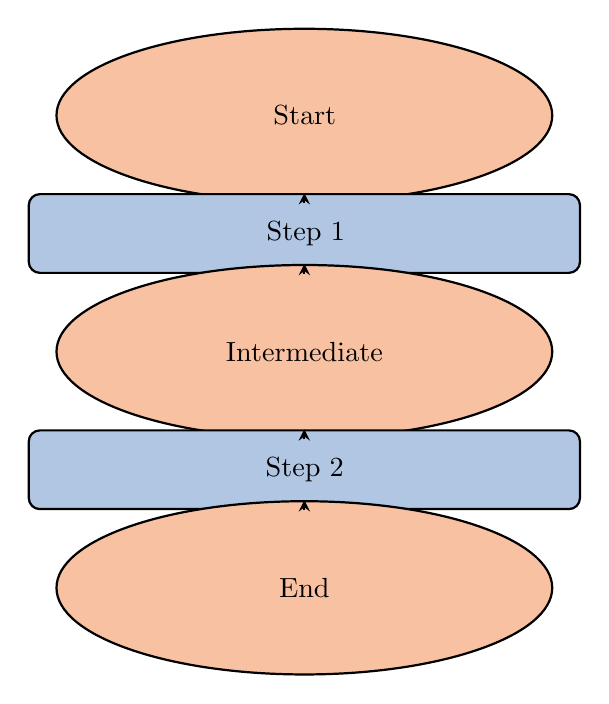
\begin{tikzpicture}[node distance=1.5cm]
\node (start) [object] {Start};
\node (step1) [process, below of=start] {Step 1};
\node (intermediate) [object, below of=step1] {Intermediate};
\node (step2) [process, below of=intermediate] {Step 2};
\node (end) [object, below of=step2]{End};

\draw [arrow] (start) -- (step1); 
\draw [arrow] (step1) -- (intermediate);
\draw [arrow] (intermediate) -- (step2); 
\draw [arrow] (step2) -- (end);
\end{tikzpicture}
\caption{A caption for the flowchart.}
\label{fig:comp}
\end{figure}

%\section{Results}

This is the results section.

\begin{align}
	F &= ma \\
	\intertext{where:}
	F &= \text{net force applied on the body [N]} \nonumber \\
	m &= \text{total mass of the body [kg]} \nonumber \\
	a &= \text{net acceleration of the body [m s}^{-2}\text{]} \nonumber
\end{align}

\begin{figure}[htbp!]
	\begin{center}
		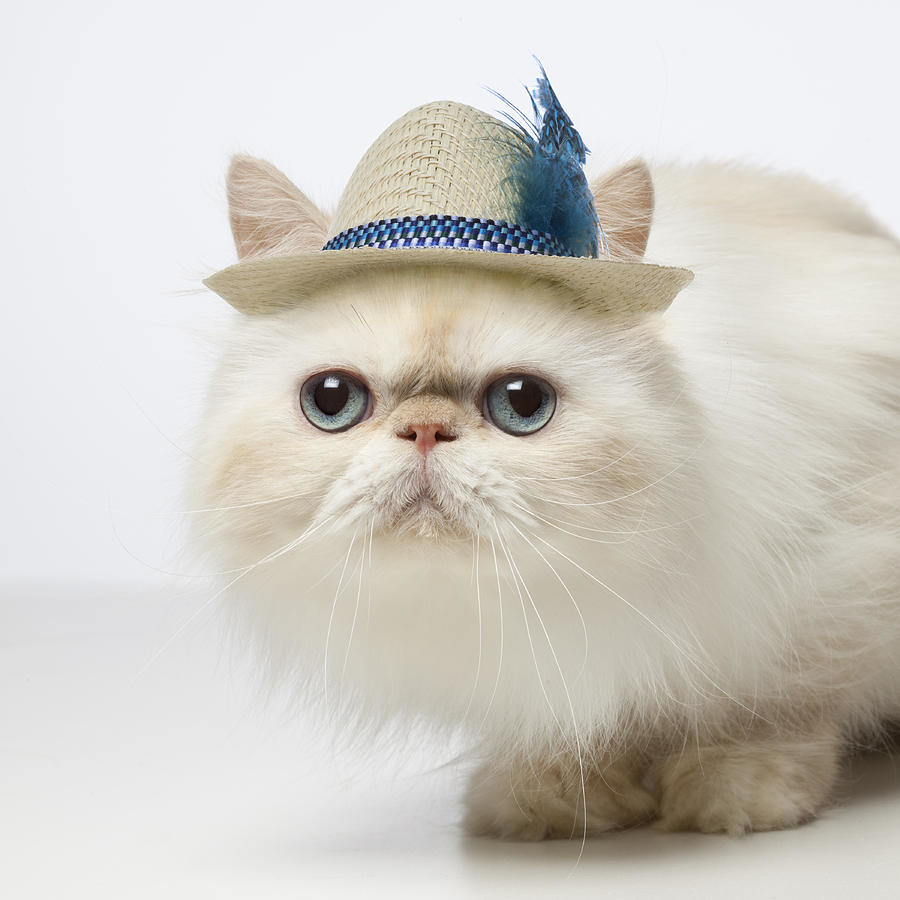
\includegraphics[scale=0.7]{./images/catinhat}
	\end{center}
	\caption{A caption for the figure.}
	\label{fig:catinhat}
\end{figure}

\begin{table}[h]
	\centering
        \caption{A caption for the table.}
\begin{tabular}{lr}
	\hline
	\textbf{Properties} & \textbf{Value} \\
	\hline
    Mass [kg] & 2,324 \\
    Height [m] & 558 \\
    Volume [m$^3$] & 4,072 \\
    \hline
\end{tabular}
\label{tab:table1}
\end {table}

%\section{Conclusions} \label{sec:conclusion}

This paper introduced the hybrid $S_N$-diffusion method for \gls{MSR} control rod neutronics
modeling. The hybrid $S_N$-diffusion method improves on the standard neutron diffusion method by
iteratively applying transport corrections generated from solving the $S_N$ neutron transport
method in subdomains containing highly neutron-absorbing control rods. The hybrid method uses the
\gls{SAAF} formulation of the $S_N$ equations, which are highly efficient and
scalable with HYPRE multigrid preconditioners \cite{hypre_hypre_2022} from PETSc.
Drift closure terms computed from the $S_N$ transport solution are passed as transport corrections
in modified forms of the neutron diffusion equations to correct flux errors in near control rods
where diffusion theory is not valid. This work also developed
an adaptive boundary coupling algorithm to couple the $S_N$ and neutron diffusion solvers. The
algorithm automatically truncates transport correction parameters near the boundaries of the
$S_N$ problem subdomain to discard inaccurate correction parameters and preserve smooth neutron
flux gradients across the interface. The $S_N$ and diffusion solvers are coupled through fixed
point iterations using the \gls{MOOSE} \texttt{MultiApp} and \texttt{Transfers} systems.

This paper presented 1-D and 2-D $k$-eigenvalue simulation results with the hybrid method on
models derived from the \gls{MSRE} reactor.
%The 1-D simulations involve six test cases with increasing
%geometric complexity modeled after the air-filled control rod thimbles, salt-graphite lattice
%structure, and vessel regions in the \gls{MSRE}.
Simulations with the OpenMC Monte Carlo neutron
transport code and the $S_8$ method in Moltres provided reference solutions for the hybrid and
neutron diffusion methods to be assessed against. Some discrepancies arose from the eight neutron
energy group structure as evidenced by differences in $k_\text{eff}$ and flux distributions between
OpenMC simulations on continuous energy (OpenMC-CE) and multigroup (OpenMC-MG) modes. Otherwise,
the multigroup $S_8$ method showed good agreement with OpenMC-MG. Although $k_\text{eff}$ estimates
from the hybrid method deviated from the $S_8$ method and OpenMC-MG by 100-400 pcm, the hybrid
method accurately reproduced control rod worth estimates within 0.5 \% of them (2-3 \% relative to
OpenMC-CE). In comparison, the neutron diffusion method fared significantly worse at 5.5 \%
relative to $S_8$ and OpenMC-MG, and 8 \% relative to OpenMC-CE. Our analyses showed little impact
on control rod worth estimates from varying the $S_N$-resolved subdomain size as long as the size
is kept constant between $k$-eigenvalue simulations used to calculate the rod worth. The hybrid
$S_N$-diffusion method exhibited a superlinear convergence rate with the number of fixed point
iterations, leading to the $k_\text{eff}$ error estimate falling below $10^{-7}$ after two
iterations.

The hybrid method maintained its accurate control rod modeling capability in 2-D simulations
involving incremental insertions of three control rods in the \gls{MSRE} model.
The hybrid method reported rod worth error magnitudes of less than 40 pcm relative to OpenMC-CE,
which were significant improvements over the neutron diffusion method error estimates ranging from
569 pcm to 1484 pcm. The hybrid method also showed significant improvements in the absolute mean
and maximum errors in fuel channel power distributions over the neutron diffusion method.

An extension to this work would be to resolve the discrepancies that persist in the hybrid method
$k_\text{eff}$ estimates of individual reactor states. Neutron leakage error at the external
boundaries is likely the most significant source of discrepancy and could be reduced through known
neutron leakage correction techniques such as group-wise or matrix albedo boundary conditions.
Further work is ongoing for the demonstration and performance characterization of the hybrid method
in $k$-eigenvalue and transient 3-D \gls{MSRE} simulations. Transient simulations under active
study include the zero-power rod drop and fractional-power reactivity insertion experiments
performed on the \gls{MSRE}. Future work would include asymmetrical power transients such as
partial channel flow blockage and potential in-core natural circulation flow following a loss of
pump power.

%The 3-D simulations in Chapter \ref{chap:msre} doubled as validation for the 3-D \gls{MSRE} model
%against reference \gls{MSRE} experimental data and the \gls{MSRE} numerical benchmark study
%\cite{fratoni_molten_2020} in
%the International Reactor Physics Experiment Evaluation Project (IRPhEP) handbook. OpenMC and
%hybrid method estimates of $k_\text{eff}$ of the \gls{MSRE} when the experiment first achieved criticality
%$k_\text{eff}$ estimates of the \gls{MSRE} at its initial critcality configuration from OpenMC, the
%hybrid method, and the neutron diffusion method in this work showed good agreement with the Serpent
%model from the \gls{MSRE} numerical benchmark. All numerical estimates exceeded the experimental
%value by 1-2 \% due to possible biases and uncertainties in the nuclear data library for graphite
%\cite{fratoni_molten_2020}. Temperature reactivity coefficient values from this work also showed
%good agreement with \gls{MSRE} data, within experimental uncertainty, with percentage discrepancies
%of about 3 \%. In the subsequent control rod worth study, OpenMC and the hybrid method showed nearly
%perfect overlap in the integral rod worth curve throughout the entire length of rod travel. Due to
%geometric approximations of the control rods in the numerical models, they overestimated the total
%rod worth relative to \gls{MSRE} data by approximately 4-5 \%. The hybrid method significantly
%outperforms the neutron diffusion method which overestimated the total worth by 21.1 \%.
%When comparing solution times, the hybrid method took approximately four times as long as the
%neutron diffusion method.
%The 3-D hybrid method simulations exhibited nearly linear scaling in strong scaling tests, which
%is promising for future projects involving larger reactor models. Some performance optimizations
%may be possible to reduce data transfer times between the $S_N$ and diffusion solvers which took
%up about 18 \% of the total solution time due to inter-processor communications.

%Lastly, Chapter \ref{chap:transient} demonstrated the hybrid method in a time-dependent simulation
%based on a \gls{MSRE} zero-power rod drop experiment \cite{prince_zero-power_1968}.
%The simulation required coupling the hybrid method solver to the pre-existing \gls{DNP} solver
%in Moltres through a nested iteration coupling setup.
%I set up the rod drop simulation through a
%$k$-eigenvalue simulation with the control rod at its initial height before using the simulation
%output as the initial condition for the time-dependent rod drop simulation. Moltres reproduced the
%expected prompt and delayed response in the integral neutron count data observed in \gls{MSRE}
%experimental data. Convergence issues midway through the simulation had a minor impact on the
%solution precision. Overall, this work successfully demonstrated a time-dependent
%reactivity-initiated simulation using the hybrid method.

%\subsection{Limitations and Future Work}

%The second \gls{VV} study verified the looped \gls{DNP} flow modeling capability in Moltres under
%steady-state and transient scenarios. In the original pump experiments, the control rod was driven
%by a ``flux servo controller'' that adjusts the rod position in response to flux changes to maintain
%criticality. Our study in this work approximated this action through $k$-eigenvalue solvers
%coupled to time-dependent \gls{DNP} flow solvers. Potential future work would be to implement a
%control system such as a PID (Proportional-Integral-Derivative) controller in combination with
%the newly-implemented hybrid method to create a more representative model of the pump experiments.
%This would enhance model validation and open up additional research directions which require a
%control system.
%
%This work implemented and verified the Spalart-Allmaras turbulence model in Moltres. The turbulence
%model \gls{VV} tests indicated significant mesh refinement requirements near the wall. Mesh
%refinement scales with the flow Reynolds number. With \gls{MSR} designs such as the \gls{MSFR}
%reaching Reynolds numbers on the order of $10^6$, future work in this area should focus on
%implementing wall functions. Wall functions eliminate the need for fine mesh near the wall by
%approximating the log-law velocity profile near the wall. Verification and demonstration of the
%turbulence model, beyond general \gls{VV} tests, in \gls{MSR} turbulent salt flow problems is also
%crucial for the continued development of Moltres as a \gls{MSR} simulation tool.

%The 3-D simulations in this work uncovered significant memory usage by the $S_N$ solver, even
%with the distributed mesh feature to spread mesh and variable data storage across the compute nodes.
%Each full-core simulation required at least 40 nodes with 512 GB memory each to run.
%This issue may be a stumbling block for using the hybrid method on smaller computing clusters that
%have less memory per processor. A custom preconditioner and solver routine in Moltres could help to
%reduce memory usage by referencing the same stored Jacobian C++ variable for neutron angular flux
%variables in the same neutron energy group and on the same \gls{FEM} quadrature point. Their
%Jacobian formulations are identical aside from the level-symmetric ordinate and weight. Another
%area for optimization in the hybrid method is reducing data transfer times between the $S_N$ and
%diffusion solvers. Due to mesh distribution, each 3-D simulation spent 18 \% of its solution time
%on data transfers between processors. This could be minimized through optimizations in the mesh
%distribution and the data transfer caching systems.
%
%Time-dependent simulations in this work uncovered two issues: rod cusping effects when a moving
%control rod does not align with the mesh interfaces, and slow solution convergence rates during
%control rod motion. While this work applied an empirical technique to correct for rod cusping
%effects, Moltres would benefit from a more robust technique for the long term. Slow solution
%convergence rates could be resolved by investigating better nested solver coupling structures to
%mitigate the effects of lagged solutions and applying solution relaxation schemes.
%
%Finally, future work could demonstrate the hybrid method to its fullest potential through the
%simulation of asymmetric reactivity-initiated transients. Asymmetry refers to significant changes
%in the neutron flux shape during a transient scenario. The core benefit of the hybrid method is
%the spatial resolution it provides to time-dependent simulations involving control rod movement.
%This objective could be met through modeling most other \gls{MSR} designs whose control and shim
%rods are not centrally located.

%\section{Acknowledgments}
This is the acknowledgements section.
Include acknowledgements for relevant funding sources and contributors for
this work. Review the \href{https://drive.google.com/open?id=1VybV0oMPiqpInTwgO0ICq0EC4AL_fGj-zbXGJAhRiVU}{how-to-acknowledge}
document for the appropriate text, which changes frequently as grants and people
come and go.


\bibliography{bibliography}

% Prof. Huff discourages appendices in journal articles.
% But, if you must, include one like so:
%\pagebreak
%
\appendix
\section{}


\end{document}
